\documentclass[fancy, twoside, mastersfancy, ms]{byuthesis}
\usepackage{bookmark}



\providecommand{\tightlist}{%
  \setlength{\itemsep}{0pt}\setlength{\parskip}{0pt}}\usepackage{longtable,booktabs,array}
\usepackage{calc} % for calculating minipage widths
% Correct order of tables after \paragraph or \subparagraph
\usepackage{etoolbox}
\makeatletter
\patchcmd\longtable{\par}{\if@noskipsec\mbox{}\fi\par}{}{}
\makeatother
% Allow footnotes in longtable head/foot
\IfFileExists{footnotehyper.sty}{\usepackage{footnotehyper}}{\usepackage{footnote}}
\makesavenoteenv{longtable}
\usepackage{graphicx}
\makeatletter
\def\maxwidth{\ifdim\Gin@nat@width>\linewidth\linewidth\else\Gin@nat@width\fi}
\def\maxheight{\ifdim\Gin@nat@height>\textheight\textheight\else\Gin@nat@height\fi}
\makeatother
% Scale images if necessary, so that they will not overflow the page
% margins by default, and it is still possible to overwrite the defaults
% using explicit options in \includegraphics[width, height, ...]{}
\setkeys{Gin}{width=\maxwidth,height=\maxheight,keepaspectratio}
% Set default figure placement to htbp
\makeatletter
\def\fps@figure{htbp}
\makeatother
% definitions for citeproc citations
\NewDocumentCommand\citeproctext{}{}
\NewDocumentCommand\citeproc{mm}{%
  \begingroup\def\citeproctext{#2}\cite{#1}\endgroup}
\makeatletter
 % allow citations to break across lines
 \let\@cite@ofmt\@firstofone
 % avoid brackets around text for \cite:
 \def\@biblabel#1{}
 \def\@cite#1#2{{#1\if@tempswa , #2\fi}}
\makeatother
\newlength{\cslhangindent}
\setlength{\cslhangindent}{1.5em}
\newlength{\csllabelwidth}
\setlength{\csllabelwidth}{3em}
\newenvironment{CSLReferences}[2] % #1 hanging-indent, #2 entry-spacing
 {\begin{list}{}{%
  \setlength{\itemindent}{0pt}
  \setlength{\leftmargin}{0pt}
  \setlength{\parsep}{0pt}
  % turn on hanging indent if param 1 is 1
  \ifodd #1
   \setlength{\leftmargin}{\cslhangindent}
   \setlength{\itemindent}{-1\cslhangindent}
  \fi
  % set entry spacing
  \setlength{\itemsep}{#2\baselineskip}}}
 {\end{list}}
\usepackage{calc}
\newcommand{\CSLBlock}[1]{\hfill\break\parbox[t]{\linewidth}{\strut\ignorespaces#1\strut}}
\newcommand{\CSLLeftMargin}[1]{\parbox[t]{\csllabelwidth}{\strut#1\strut}}
\newcommand{\CSLRightInline}[1]{\parbox[t]{\linewidth - \csllabelwidth}{\strut#1\strut}}
\newcommand{\CSLIndent}[1]{\hspace{\cslhangindent}#1}

\usepackage{flafter}
\usepackage{float}
\usepackage[section]{placeins}
\floatplacement{table}{htbp}
\usepackage{booktabs}
\usepackage{longtable}
\usepackage{array}
\usepackage{multirow}
\usepackage{wrapfig}
\usepackage{float}
\usepackage{colortbl}
\usepackage{pdflscape}
\usepackage{tabu}
\usepackage{threeparttable}
\usepackage{threeparttablex}
\usepackage[normalem]{ulem}
\usepackage{makecell}
\usepackage{xcolor}
\usepackage{siunitx}
\usepackage{booktabs}
\usepackage{longtable}
\usepackage{array}
\usepackage{multirow}
\usepackage{wrapfig}
\usepackage{float}
\usepackage{colortbl}
\usepackage{pdflscape}
\usepackage{tabu}
\usepackage{threeparttable}
\usepackage{threeparttablex}
\usepackage[normalem]{ulem}
\usepackage[utf8]{inputenc}
\usepackage{makecell}
\usepackage{xcolor}
\makeatletter
\@ifpackageloaded{bookmark}{}{\usepackage{bookmark}}
\makeatother
\makeatletter
\@ifpackageloaded{caption}{}{\usepackage{caption}}
\AtBeginDocument{%
\ifdefined\contentsname
  \renewcommand*\contentsname{Table of contents}
\else
  \newcommand\contentsname{Table of contents}
\fi
\ifdefined\listfigurename
  \renewcommand*\listfigurename{List of Figures}
\else
  \newcommand\listfigurename{List of Figures}
\fi
\ifdefined\listtablename
  \renewcommand*\listtablename{List of Tables}
\else
  \newcommand\listtablename{List of Tables}
\fi
\ifdefined\figurename
  \renewcommand*\figurename{Figure}
\else
  \newcommand\figurename{Figure}
\fi
\ifdefined\tablename
  \renewcommand*\tablename{Table}
\else
  \newcommand\tablename{Table}
\fi
}
\@ifpackageloaded{float}{}{\usepackage{float}}
\floatstyle{ruled}
\@ifundefined{c@chapter}{\newfloat{codelisting}{h}{lop}}{\newfloat{codelisting}{h}{lop}[chapter]}
\floatname{codelisting}{Listing}
\newcommand*\listoflistings{\listof{codelisting}{List of Listings}}
\makeatother
\makeatletter
\makeatother
\makeatletter
\@ifpackageloaded{caption}{}{\usepackage{caption}}
\@ifpackageloaded{subcaption}{}{\usepackage{subcaption}}
\makeatother

\title{A Comparative Illustration of Trip- and\\
Activity-Based Modeling Techniques}
\author{Hayden Atchley}
%\author{Hayden AtchleyKamryn MansfieldGregory S. Macfarlane}

% On the custom title page, use the same title, but format as you like
\customtitle{A Comparative Illustration of\\
Trip- and Activity-Based\\
Modeling Techniques}

% This is the date of graduation
\date{27 May 2024}

% If your degree is not a PhD or MS, then you can overwrite the degree using
% the \degree command: \degree{Bachelors of Basics}

% Your department
\department{Civil and Construction Engineering}

% The names of your committee members
\committeechair{Gregory S. Macfarlane}
  \committeemember{Grant G. Schultz}
  \committeemember{Gustavious P. Williams}

\keywords{
    travel demand model; activity-based model;
    ActivitySim
}

\begin{document}

\frontmatter
\titlepage
\cleardoublepage

\customtitlepage
\cleardoublepage


  \begin{abstract}
Activity-based travel demand models (ABMs) are generally considered
superior to their trip-based counterparts, as ABMs explicitly model
individuals in contrast to the aggregate nature of trip-based models.
There have been a number of comparisons between trip- and activity-based
models, but these comparisons focus almost exclusively on the technical
ability of the two model types, while not considering the practical
benefits an ABM may or may not have to a transportation agency. This
research performs a more holistic comparison between trip- and
activity-based models, focused specifically on the practical differences
between model types, both in terms of usability and capability for
complex analysis. We use the existing Wasatch Front Regoinal Council
(WFRC) model as a representative trip-based model, and an ActivitySim
implementation in the same area as a representative ABM. We create three
hypothetical scenarios in both models: a change in land use, an
improvement to commuter rail service, and an increase in remote work. We
discuss the process of creating each scenario in both models, and
perform several example analyses with each scenario and model. Notably,
we find that many commonly-cited reasons for the lack of ABM adoption
may not be as applicable as previously thought. ABMs are often
considered more complicated than trip-based models, requiring more data
and computational resources. While ABMs do require more input data, we
found that in our case the complexity of the model and the computational
resources required were similar between model types. Additionally, the
ABM allows for much more intuitive and straightforward interpretation of
results.
\end{abstract}
\cleardoublepage

\begin{acknowledgments}
I would like to acknowledge the Utah Department of Transportation for
providing funding for this research. Additionally, I would like to thank
the modeling teams at the Utah Department of Transportation, Wasatch
Front Regional Council, Mountainland Association of Governments, and
Fehr \& Peers for their help and input at several stages of this
project. I would specifically like to thank Chad Worthen and Chris Day
at Wasatch Front Regional Council for answering my questions about their
travel demand model. I would also like to thank my peers in the BYU
transportation lab for their friendship and support, and especially for
their help dealing with miscellaneous issues that arose throughout this
project. Lastly, I would like to especially thank my graduate advisor,
Greg Macfarlane, for his support and encouragement.
\end{acknowledgments}
\cleardoublepage

	\tableofcontents*
	\cleardoublepage

	\listoffigures
	\cleardoublepage

	\listoftables
	\cleardoublepage

\bookmarksetup{startatroot}

\chapter*{List of Acronyms}\label{list-of-acronyms}
\addcontentsline{toc}{chapter}{List of Acronyms}

\markboth{List of Acronyms}{List of Acronyms}

\begin{description}
\tightlist
\item[\phantomsection\label{acronyms_ABM}{ABM}]
activity-based model
\item[\phantomsection\label{acronyms_ASC}{ASC}]
alternative-specific constant
\item[\phantomsection\label{acronyms_CRT}{CRT}]
commuter rail transit
\item[\phantomsection\label{acronyms_DAP}{DAP}]
daily activity pattern
\item[\phantomsection\label{acronyms_PUMA}{PUMA}]
Public Use Microdata Area
\item[\phantomsection\label{acronyms_SEMCOG}{SEMCOG}]
Southeast Michigan Council of Governments
\item[\phantomsection\label{acronyms_TAZ}{TAZ}]
transportation analysis zone
\item[\phantomsection\label{acronyms_WFRC}{WFRC}]
Wasatch Front Regional Council
\end{description}
\cleardoublepage

\mainmatter

\bookmarksetup{startatroot}

\chapter{Introduction}\label{sec-introduction}

Activity-based models (ABMs) have been championed by researchers and
many practitioners as being theoretically superior to the trip-based
models historically used in transportation planning efforts since the
1950s (Rasouli and Timmermans 2014). ABMs explicitly model individuals,
in contrast to the aggregate nature of trip-based models, and so in
theory are able to represent travel behavior more accurately.
Additionally, the focus on individuals in an ABM can allow for more
detailed post-hoc analysis of model outputs compared to a trip-based
model.

There have been a number of comparisons and case studies between trip-
and activity-based models (see e.g. Ferdous et al. 2012; Zhong et al.
2015; and Mouw 2022), but these comparisons focus almost exclusively on
the technical ability of the two model types. Though there are potential
\emph{theoretical} benefits to ABMs over trip-based models, there is
little discussion in the literature of the \emph{practical} benefits an
ABM has, if any. In fact, while trip-based models are almost ubiquitous
among transportation agencies, many agencies have delayed or declined to
transition to an ABM citing additional data requirements, staff
training, computational resources, and related concerns (Miller 2023).

In this research, we perform a more holistic comparison of ABMs to
trip-based models, with a particular focus on the practical
considerations an agency would need to make in transitioning to an ABM.
We additionally discuss the potential practical advantages regarding the
quality and characteristics of travel analyses that an ABM allows.
Though this research occasionally makes quantitative comparisons between
model types, we do not focus heavily on model \emph{accuracy} (either to
each other or to observed data), as this can be adjusted in any model
type through model calibration. Instead, this research seeks to
illustrate the differences between trip- and activity-based models in a
way that would be practically useful to an agency considering
transitioning to an ABM, noting potential pain points both in the
literature and in our experience in this research itself.

To compare the model types, we first identify three main goals of travel
demand modeling, which are to model travel behavior in response to
changes in land use, transportation infrastructure, and social/economic
factors. We then create three hypothetical model scenarios, one for each
goal identified. These scenarios are the addition of a new development,
an increase in commuter rail service, and an increase in remote work,
respectively. Each of these scenarios is created in both a trip-based
and activity-based model representing the Wasatch Front (Salt Lake City)
region of Utah, USA. We discuss the process of implementing each
scenario, as well as perform a variety of post-hoc analyses, for both
model types.

The document proceeds in a typical fashion: Chapter~\ref{sec-literature}
provides an overview of the literature discussing the differences
between trip-based models and ABMs, including the theoretical and
analytical benefits of each framework. Chapter~\ref{sec-methods} first
describes the models used in this research, namely the existing regional
trip-based model and an activity-based model constructed to support
research activities in the region; this section also describes the
scenarios designed to test the usefulness and applicability of the
different model frameworks. Chapters \ref{sec-landuse}--\ref{sec-wfh}
describe the findings from each scenario, alongside a discussion of
related limitations and implications. Chapter~\ref{sec-conclusions}
provides a summary of our findings and a discussion of our conclusions,
along with a set of recommendations.

\bookmarksetup{startatroot}

\chapter{Literature Review}\label{sec-literature}

Travel demand modeling in the modern sense has its origins in the
1950's, with the Chicago Area Transportation Study (Chicago Area
Transportation Study 1959) being one of the first urban planning studies
to use the now-ubiquitous ``four-step'' modeling framework (McNally
2007). Up to this point, most urban transportation planning used
existing demand or uniform-growth travel forecasts to model travel
demand, but the Chicago Study used a combination of trip generation,
trip distribution, modal split, and network assignment models to more
accurately represent travel behavior (Weiner 1997). Since then, there
have been numerous studies iterating on the ``four-step'' (more
appropriately termed ``trip-based'') framework, and trip-based models
are now the primary tool used in forecasting travel demand across the
United States (Park et al. 2020).

These trip-based models are not without problems, however. Rasouli and
Timmermans (2014) give several shortcomings of trip-based models. First,
they use several sub-models that are (implicitly or explicitly) assumed
independent, and this can result in a lack of consistency or integrity
between sub-models. For example, the assumed value of time in the mode
choice model might be radically different than the assumed value of time
in the tolling assignment model. Second, these models are strongly
aggregate in nature, which can cause significant aggregation bias with
high and low values excluded. Finally, they lack ``behavioral
realism''---that is, they do not have a concept of individuals making
decisions, which is what travel behavior actually is.

Jones (1979) proposed an alternative to the trip-based paradigm, namely
an ``activity-based'' framework that models daily activity patterns at
an individual rather than aggregate level. An activity-based model (ABM)
places the focus on ``activities'' rather than ``trips'' as the basic
unit of analysis, and predicts a sequence of activities for each
individual and household, with information such as activity location,
start time, and duration, using a high level of temporal and spatial
granularity. ``Trips'' are then journeys from one activity to the next
(Pinjari and Bhat 2011). By adopting this activity-centric framework,
ABMs provide a more consistent and comprehensive representation of
travel behavior. They take into account complex dependencies and
interactions within the model as a whole and at an individual level.
ABMs acknowledge that travel choices are not made in isolation, but
rather influenced by the preceding activities. This means that e.g.~if
an individual takes transit to work, they will not be able to drive
home. ABMs therefore attempt to present a more conceptually accurate
model of actual travel behavior than traditional trip-based models.

Despite these advantages, many agencies have yet to adopt ABMs, and
instead continue to use trip-based models (Miller 2023). While ABMs are
superior in certain aspects, they also have disadvantages, such as
requiring more detailed input data and greater computational resources.
It is also not always clear if ABMs provide substantially better
forecasts than their trip-based counterparts, nor if this tradeoff is
worth the increased costs for every agency. This literature review
presents an overview of both modeling frameworks, and discusses the
advantages and disadvantages of using an ABM.

\section{Overview of Model Types}\label{overview-of-model-types}

Trip-based models are often referred to as ``four-step'' models due to
their four fundamental sub-models: trip generation, trip distribution,
mode choice, and network assignment (National Academies 2012 p. 28).
Models can be more complicated than these four steps, possibly including
integration with a land use forecast, iteration between mode and
destination choice, etc., but the ``four steps'' are the central
component of any of these models (McNally 2007).

In a typical trip-based model, travel demand is predicted based on
aggregate population data, often delineated by
transportation analysis zone (TAZ). Each sub-model relies on this
aggregate data; for example, the modal split sub-model will often use
average TAZ income as an input (National Academies 2012 p. 14). Many
trip-based models include a disaggregation step, where this aggregate
data is segmented along variables such as household size and vehicle
ownership. Regardless of the segmentation variables used in the first
three model steps, the resulting trip matrices by mode and time of day
are then assigned to a transportation network.

Activity-based models differ significantly from this approach. Rather
than using aggregate data, ABMs use data representing an actual or
synthetic population, with individual person and household data (Vovsha
et al. 2005). These models use an activity or tour scheduler to assign a
daily activity pattern (DAP) of zero or more tours to each individual
(\emph{n.b.} a tour is a series of trips that begin and end at home).
These DAPs are restricted temporally, spatially, and modally; i.e., each
person has a logical and followable sequence of trips and activities
(Bowman 1998). A ``drive alone'' trip from work to lunch, for example,
cannot be made if transit was taken to work. ABMs output a list of tours
and trips by person, time, location, and type, and these can then be
assigned to a transportation network in a similar manner as in a
trip-based model. In effect, an ABM replaces the first ``three'' steps
of the traditional ``four-step'' approach.

\section{Comparison of Modeling
Frameworks}\label{comparison-of-modeling-frameworks}

In discussing the differences between ABMs and trip-based models, there
are really two comparisons that need to be made: how the population data
is structured, and how travel is organized. Trip-based models generally
use aggregate population data while ABMs use a synthetic population, and
trip-based models organize travel into trips while ABMs organize travel
into activities and tours. The following sections explain these aspects
of travel demand modeling and discuss the claimed advantages and
disadvantages of each model type.

\subsection{Population Data}\label{population-data}

The aggregate population data used in trip-based models can vary in
origin and level of detail, but the basic concept is the same: the study
area is organized into generally small zones, and certain demographic
and socioeconomic data is known or obtained for each zone (National
Academies 2012 p. 14). This includes data such as number of households,
average household income, population, number of workers, etc. Rather
than predict travel behavior using only this zone-level aggregate data,
many models include a ``disaggregation'' step, which classifies the
households in a zone along variables such as household size, vehicle
ownership, and number of workers. For example, a 1000-household zone
with an average household size of 3 may be classified into 500 2-person
and 500 4-person households.\footnote{The specific method for
  classifying households may differ between models, so different models
  will have a different distribution of households along each variable
  used for classification.} This disaggregation is useful, as travel
behavior (such as the number of trips made) can vary significantly based
on a household's classification.

Subsequent model steps then use this disaggregated data in their
estimations. A 2-worker, 1-vehicle household, for example, may be
modeled to make 3.8 work trips on an average weekday, while a 1-worker,
1-vehicle household may make fewer. The trips are then added to obtain
the total number of trips produced by each zone (National Academies 2012
p. 37).

This approach is relatively straightforward: the required input data is
usually easy to obtain, the trip generation models are often simple, and
it is computationally inexpensive (National Academies 2012). However,
the types of analyses possible are limited by the initial segmentation
of the aggregate population data. An analysis based on parents'/adults'
highest received education, for example, would require determining the
number of households in each TAZ with each possible combination of
education level. This can theoretically be done, but more detailed and
varied analyses would require more levels of segmentation, greatly
increasing the number of classifications needed. Since these
segmentations need to be carried through each model step, trip rates,
mode choice equations, etc. need to be estimated for every
classification, and while relevant real-world data may exist, sample
sizes approach zero very quickly, and so the estimates have little
statistical value (Moeckel et al. 2020; National Academies 2012).
Further, combining these segmentations at any point precludes that
segmentation from use in subsequent model steps as well as in any
post-hoc analysis.

This becomes a particular issue in equity analysis because it is perhaps
impossible to determine equitable distribution of ``winners'' and
``losers'' of a potential policy without using demographic variables in
the trip generation and destination and mode choice steps (Bills and
Walker 2017). Though many studies have shown that trip production and
mode choice behavior differ by ethnic group even after controlling for
income (Bhat and Naumann 2013; Yum 2020; Zmud and Arce 2001), including
such variables in trip-based models is problematic. Does coding such a
variable in a mode choice model represent discrimination? Or does doing
so assert that present differences resulting from unequal opportunity
will persist into future planning years? Regardless of the reasons for
their exclusion, these variables consequently cannot be used in a
post-hoc analysis of a transportation policy because the trip matrices
do not contain the adequate segmentation.

An alternative approach to population data, and the approach that ABMs
use, is to use a full synthetic population. A synthetic population takes
demographic and socioeconomic data at various levels of detail to create
a ``population'' with generally the same attributes as the study area
(National Academies 2012 p. 93). The goal is to have a population that
is functionally similar to the actual population, but without the
privacy concerns of using real individual household data. Castiglione et
al. (2006) argue that the major advantage with this approach is that the
demographic and socioeconomic data is known at the person and household
level, rather than the zone level, and this data remains available
throughout the modeling process. This allows, for example, an equity
analysis to identify the ``winners'' and ``losers'' of a proposed
development without needing to encode demographic variables into each
step of the model.

Bills and Walker (2017) used the 2000 Bay Area Travel Survey to create a
synthetic population and compare the effects that certain scenarios had
on high income and low income populations. With a 20\% reduction in
travel cost, they found that high income workers benefited more than low
income workers. They did similar comparisons for scenarios involving
reduced travel times for different mode choices and saw the effects each
scenario had on the high and low income workers. These types of
analysis, which are difficult with aggregate population data, can be
very valuable in transportation planning and policy making, particularly
when equity is a priority.

It is important to note that while many connect them only with ABMs,
synthetic populations can be used in running trip-based models as well.
Trip-based models using a synthetic population---often called trip-based
microsimulation models---do exist (see Walker (2005) and Moeckel et al.
(2020)), but these are relatively rare.

Figure~\ref{fig-pipeline-example} gives a visualization of an example
``information pipeline'' for a model using aggregate data and a model
using a synthetic population. In the aggregate data model, it is
impossible to know which trips are made by e.g.~2-worker, 1-vehicle,
low-income households after the mode choice step; it only describes
which trips are made by households with fewer vehicles than workers.
With a synthetic population, however, \emph{individuals} are being
modeled, and so each trip can be traced to a specific person. All
information is known at each point in the model regardless of which data
is used in previous steps.

\begin{figure}

\begin{minipage}{\linewidth}

\centering{

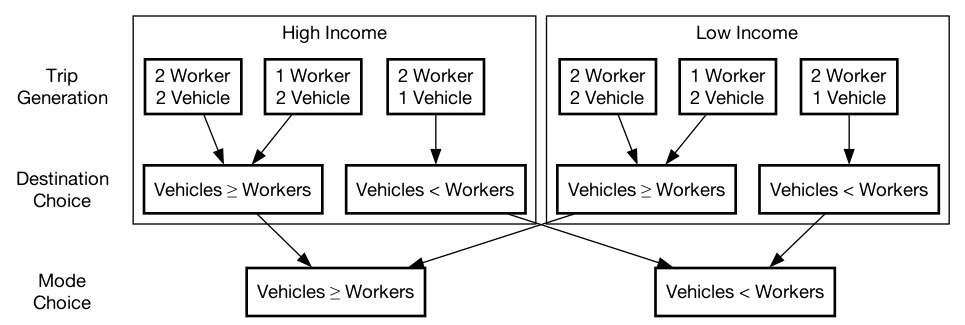
\includegraphics{qmd/../images/aggregate.png}

}

\subcaption{\label{fig-pipeline-example-1}Aggregate data}

\end{minipage}%
\newline
\begin{minipage}{\linewidth}

\centering{

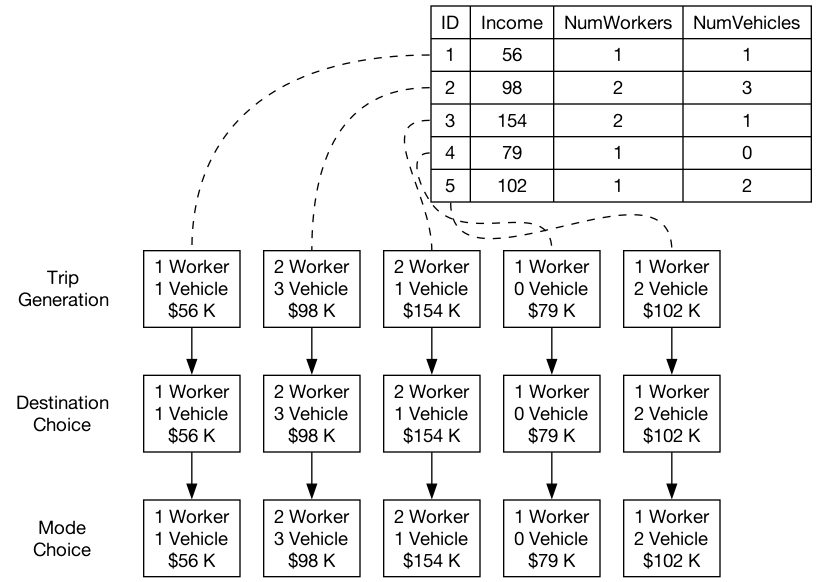
\includegraphics{qmd/../images/synthetic.png}

}

\subcaption{\label{fig-pipeline-example-2}Synthetic population}

\end{minipage}%

\caption{\label{fig-pipeline-example}Example ``information pipeline''
for aggregate data vs.~a synthetic population.}

\end{figure}%

\subsection{Travel Behavior}\label{travel-behavior}

The other primary difference between trip-based models and ABMs---and
the main difference from trip-based microsimulation models---is that
ABMs organize travel into ``tours'', a sequence of trips that begin and
end at the home, rather than just trips. It should be noted that Miller
(2023) argues that many current ``activity-based'' models ought to be
labeled ``tour-based'' due to this focus on building tours. This is
contrasted with ``activity scheduling'' models, in which activity
participation is modeled explicitly and trips emerge as the means to get
from one activity to the next. However, in practice there are few true
``activity scheduling'' models, and the term ``activity-based'' is
commonly used to refer to both activity scheduling and tour-based
models.

In a typical trip-based model, trips are forecasted based on empirical
trip rates, usually by trip purpose and by household type (for example,
low-income, 1-vehicle households make a certain number of ``home-based
work'' trips) (McNally 2007). These trips are then assigned an origin
and destination, mode, and often a time of day (peak/off-peak, etc.),
resulting in a list of trips between each zone by mode and purpose. A
trip-based microsimulation model may use choice models rather than
aggregate data for some of the model steps (Moeckel et al. 2020), but
the end result is similar: a list of trips by person, noting mode and
purpose. However, this trip list may be inconsistent, and the forecasted
trips may not be physically possible to complete in any sequence, as
there is no sense of ``trip-chaining''. The hope, though, is that over
an entire population the inconsistencies would cancel out, leaving an
overall accurate forecast.

ABMs, on the other hand, model \emph{tours} rather than trips. This
attempts to create consistency in trip origins/destinations, mode
choice, and time of day: since each trip is a part of a ``chain''
(tour), the trips within a tour are dependent on each other (Rasouli and
Timmermans 2014). The open-source ABM ActivitySim (Association of
Metropolitan Planning Organizations 2023a), for example, has a
tour-scheduling model that determines the number of ``mandatory'' (work,
school, etc.) and ``discretionary'' tours each individual will make, and
performs tour-level mode and destination choice for each tour. After the
tour-level decisions are made, trip-level mode/destination choice is
done for each trip in the tour, including the possible addition of
subtours (see Vovsha et al. (2005), fig.~18.1).

Figures \ref{fig-network-aggregate} and \ref{fig-network-synth} show an
example of the trips distributed across several TAZs in the various
model types. Figure~\ref{fig-network-aggregate} depicts the distribution
in a typical trip-based model where the total number of trips between
each zone is modeled. With these results, the mode and purpose of each
trip is known, but, with aggregate data, there is no way of telling who
made which trips other than the segmentation in the previous steps (see
Figure~\ref{fig-pipeline-example-1}). It is also not possible to
construct a coherent daily list of trips for individuals.
Figure~\ref{fig-network-synth}, on the other hand, depicts visual
representations of an \emph{individual's} travel made possible by the
use of a synthetic population. Figure~\ref{fig-network-synth-1} depicts
the trip distribution that could be given for an individual in a
trip-based microsimulation model. Though each individual's trips are
known, there is no guarantee of consistency between trips. For example,
it could predict that the individual takes transit to work but then
drives home or that the individual makes two recreational trips without
ever making a return trip. The activity-based approach, depicted in
Figure~\ref{fig-network-synth-2}, attempts to add this consistency by
modeling tours, and only generating trips consistent with each tour.

\begin{figure}

\centering{

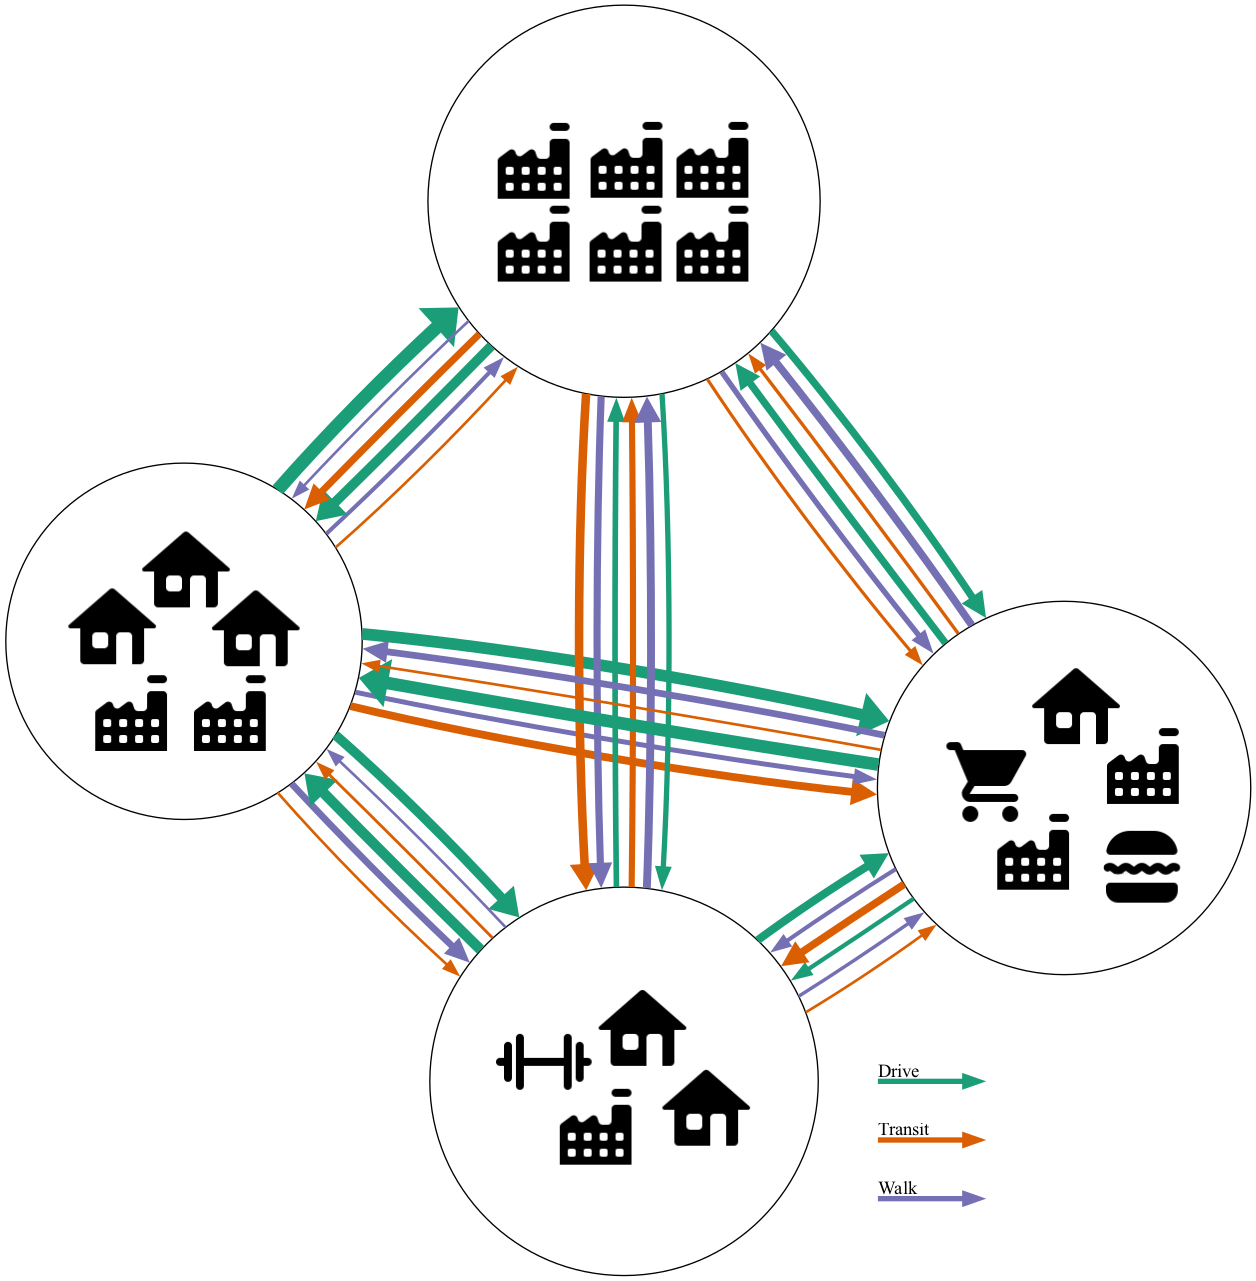
\includegraphics{qmd/../images/tbm.png}

}

\caption[Example network assignment using aggregate
data.]{\label{fig-network-aggregate}Example trip distribution using
aggregate data. There is little information on who is making which
trips, and it is not known how trips are related to each other.}

\end{figure}%

\begin{figure}

\begin{minipage}{0.50\linewidth}

\centering{

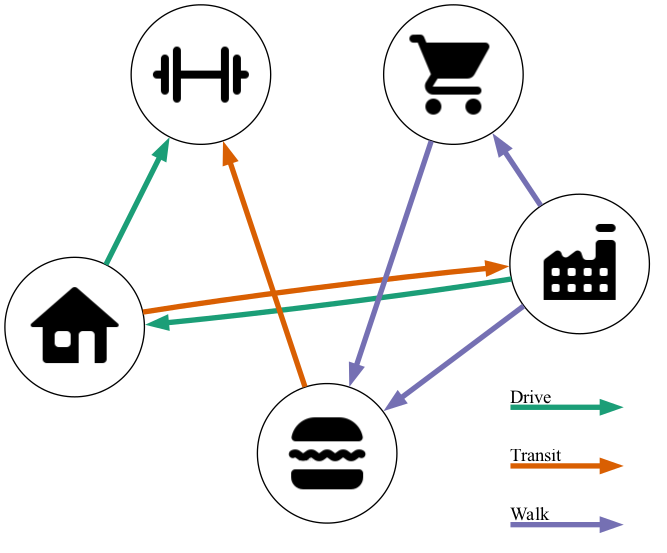
\includegraphics{qmd/./../images/trip.png}

}

\subcaption{\label{fig-network-synth-1}Trip-based microsimulation}

\end{minipage}%
%
\begin{minipage}{0.50\linewidth}

\centering{

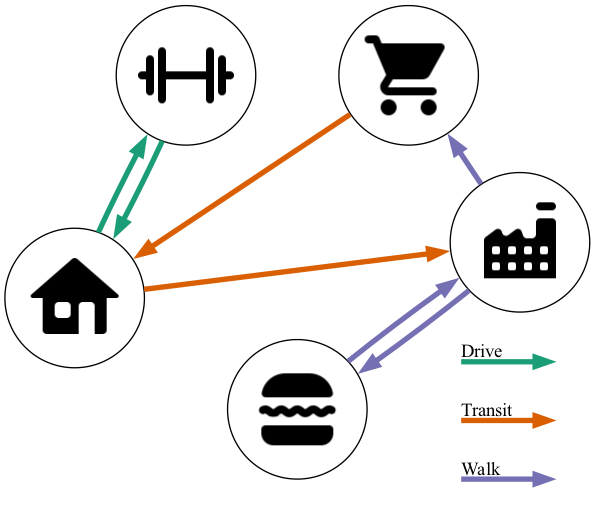
\includegraphics{qmd/./../images/tour.png}

}

\subcaption{\label{fig-network-synth-2}Activity (tour)-based}

\end{minipage}%

\caption{\label{fig-network-synth}Example trip distribution using a
synthetic population allows an individual's travel to be tracked. In the
tour-based approach, an attempt is made to make the trips consistent
with each other, while the trip-based approach may not be consistent.}

\end{figure}%

In addition to intra-person dependencies, Rasouli and Timmermans (2014)
note that ABMs can model dependencies between members of a household as
well. A vehicle can't be used by multiple people in the same household
at the same time to travel to different destinations. Because the people
within the household will have travel patterns that depend on the
patterns of others in the household, a policy affecting one person in
the household can affect everyone in the household no matter how
directly the policy connects to them (Macfarlane and Lant 2023; Vovsha
et al. 2005). These effects aren't possible to forecast in a trip-based
model.

Another advantage of organizing travel into tours comes regarding
accessibility analyses. Dong et al. (2006) note that when trip-based
models are used to analyze accessibility, each zone must be analyzed
independently of travel behavior. This approach only analyzes zones'
proximity to each other and does not take into account individual travel
patterns. They argue that this is a limited view of accessibility, and
discuss the ``activity-based accessibility measure'', which is evaluated
based on all trips in a day rather than particular trips. As an example,
if an individual doesn't live within a 20-minute drive of a grocery
store, traditional measures might rate this as poor accessibility.
However, if a grocery store lies on their path between work and home,
then in reality the accessibility should be rated much higher. Overall,
they found that the ``activity-based accessibility measure'' predicts
more reasonable accessibility outcomes compared to traditional measures.

\section{Lack of ABM Adoption}\label{sec-literature-lack-of-adpotion}

Though ABMs have many clear theoretical advantages over trip-based
models, adoption among agencies has been relatively slow. Many ABMs are
implemented in proprietary software, which creates difficulty in
maintaining and iterating on the model, Miller (2023) argues. Even in an
open-source model like ActivitySim (Association of Metropolitan Planning
Organizations 2023a), Miller notes several disadvantages of ABMs:

\begin{itemize}
\item
  Computational inefficiency and complicated program design: ABMs take
  more time, more computing power, and more money to run. This is
  because the synthetic population needed to run an ABM uses much more
  data. In areas with thousands of TAZs and millions of people, a
  supercomputer is needed, and it will cost much more than what is spent
  to run trip-based models. If a region can see similar results using a
  trip-based model, they may decide not to invest in an ABM.
\item
  Absence of a standard model system: The modeling systems are often
  designed with different approaches and for specific areas making it
  hard to transfer from one urban area to another. This also makes it
  difficult for agencies to determine which approach is the best and
  decide which to implement. In relation to this, Miller also states
  that the pressures of publishing unique and ground-breaking research
  in academia can deter researchers from converging towards best
  theories and methods.
\item
  Lack of resources: Most of these models were developed in academic
  settings which often lack resources, and possibly desire, to put them
  into practice. This leaves it up to governments and consultants to put
  the models into practice, but they can be hesitant to promote software
  development and to invest in new systems.
\end{itemize}

For these reasons, as well as the inertia of current practices, many
agencies and organizations in the US remain using trip-based models for
demand forecasting and policy analysis.

\section{Research Gap}\label{sec-literature-research-gap}

Although there has been much research on ABMs and their theoretical
advantages, practical comparisons of the model frameworks have been
limited. It is often taken as given that ABMs are unilaterally superior
to traditional trip-based models due to their better theoretical
foundation, but it is not clear if that better foundation always yields
better results in terms of analytical flexibility or policy outcomes.
Ferdous et al. (2012) compared the trip- and activity-based model
frameworks of the Mid-Ohio Regional Planning Commission and found that
the ABM was slightly more accurate to observed data at the region level,
but about the same at the project level. Zhong et al. (2015) found
significant differences in the predictions from an ABM compared to a
trip-based model in Tampa, Florida, but Mouw (2022) found that both
model types had similar prediction quality when compared with observed
data.

These comparisons have somewhat contradictory findings, and certainly do
not present an overwhelming victory for ABMs. Each of these comparisons,
however, is focused on the \emph{accuracy} of the two frameworks, but do
not address the methodological differences between model types. What
types of data collection/synthesis are needed for each model type? Are
there analyses that can only be done through (or that are made easier
by) one of the model types? What would an agency need in order to
transition from a trip-based model to an ABM? Are certain types of
scenarios suited to one model type? Though some of these questions have
been discussed (see e.g. Lemp et al. 2007), a holistic methodological
comparison is lacking. The answers in the current literature are mainly
theoretical, with little use to an agency considering the transition.
Additionally, much of the existing literature comparing the two model
types is outdated, and the technology of both model types may have
significantly changed in recent years.

This research aims to answer these questions by providing a side-by-side
comparison of a potential trip-based and activity-based modeling
methodology. Several ``proposed development'' scenarios are run in each
model, and the strengths and weaknesses of each approach are compared.
It is important to note that this research is not focused on model
accuracy, as in any model type this can be adjusted dramatically through
calibration efforts. Rather, the focus is on the methodological
differences between the approaches, and the types of analyses that can
be done with each model type.

\bookmarksetup{startatroot}

\chapter{Methodology}\label{sec-methods}

This paper seeks to compare methodological differences between trip- and
activity-based modeling frameworks. Both model types have a wide variety
of implementations, as individual agencies will adjust the basic model
framework to match their specific needs. It would be unreasonable to
compare each of the various implementations of both model types.
Instead, a representative model is used for both types, and care is
taken to note when results apply to trip- or activity-based models
generally, and when results are specific to the models used.

The representative trip-based model is the 2019 Wasatch Front Regional
Council (WFRC) travel demand model, which covers much of the Salt Lake
City-Provo-Ogden, Utah Combined Statistical Area. An ActivitySim
implementation in the same study area is used as a representative
activity-based model (ABM). Both models are discussed in detail in the
following sections.

Note that the focus is not on comparing model accuracy or performance,
but rather on comparing the process of using each model, including the
types of analyses that can be performed. There are therefore few direct
comparisons of model outputs between each type. Instead, this research
highlights the strengths and weaknesses of each model type in planning
and policy analysis, and illustrates these differences.

\section{WFRC Model}\label{wfrc-model}

The WFRC model is implemented in the CUBE software by Bentley (Bentley
Systems 2023), and is currently used by WFRC for modeling travel in the
Salt Lake City, Utah area. WFRC provided the model directly, including
land use forecasts and the current long-range transportation plan. The
model is taken essentially as-is, with no changes other than those noted
in Chapters \ref{sec-landuse}--\ref{sec-wfh} to implement the scenarios
studied in this research.

The WFRC model, like many trip-based models, requires the following
inputs:

\begin{itemize}
\tightlist
\item
  Land use data, including information about population, employment, and
  socioeconomic variables such as income, delineated by transportation
  analysis zone (TAZ). This is provided by WFRC directly, as an output
  of their land use forecasting model(s).
\item
  Travel skims detailing travel time, cost, etc. between each
  origin-destination pair of TAZs. The WFRC model uses an iterative
  process of assigning volumes to the transportation network and
  recalculating the skims, which are used in the destination and mode
  choice model steps.
\item
  Transportation networks, including highway, transit,
  etc.\textbackslash@ networks which connect the TAZs to each other.
  These networks contain information such as link speed and capacity.
  Though the WFRC model assigns travel volumes to the network, this
  paper does not analyze the model's network assignment results.
  However, the network volumes are still used to calculate the loaded
  network skims.
\item
  Lookup tables, used in many model steps for information such as trip
  rates by household type. These are taken directly from the WFRC model
  without modification.
\item
  Model constants and coefficients, which some model steps such as mode
  choice require for calibration. These are also taken directly from the
  WFRC model.
\end{itemize}

Figure~\ref{fig-wfrc-flowchart} gives an overview of the WFRC model,
showing broad model steps in a flowchart. Like many trip-based models,
the WFRC model follows the ``four-step'' approach and has main steps of
trip generation, trip distribution, mode choice, and network assignment.
The model also includes a disaggregation step at the beginning where the
TAZ-level data is used via lookup tables to estimate the number of
households by size, income group, number of workers, and auto ownership.
This does not create a fully synthetic or disaggregated population, but
is more segmented than the initial TAZ-level data.

\begin{figure}

\centering{

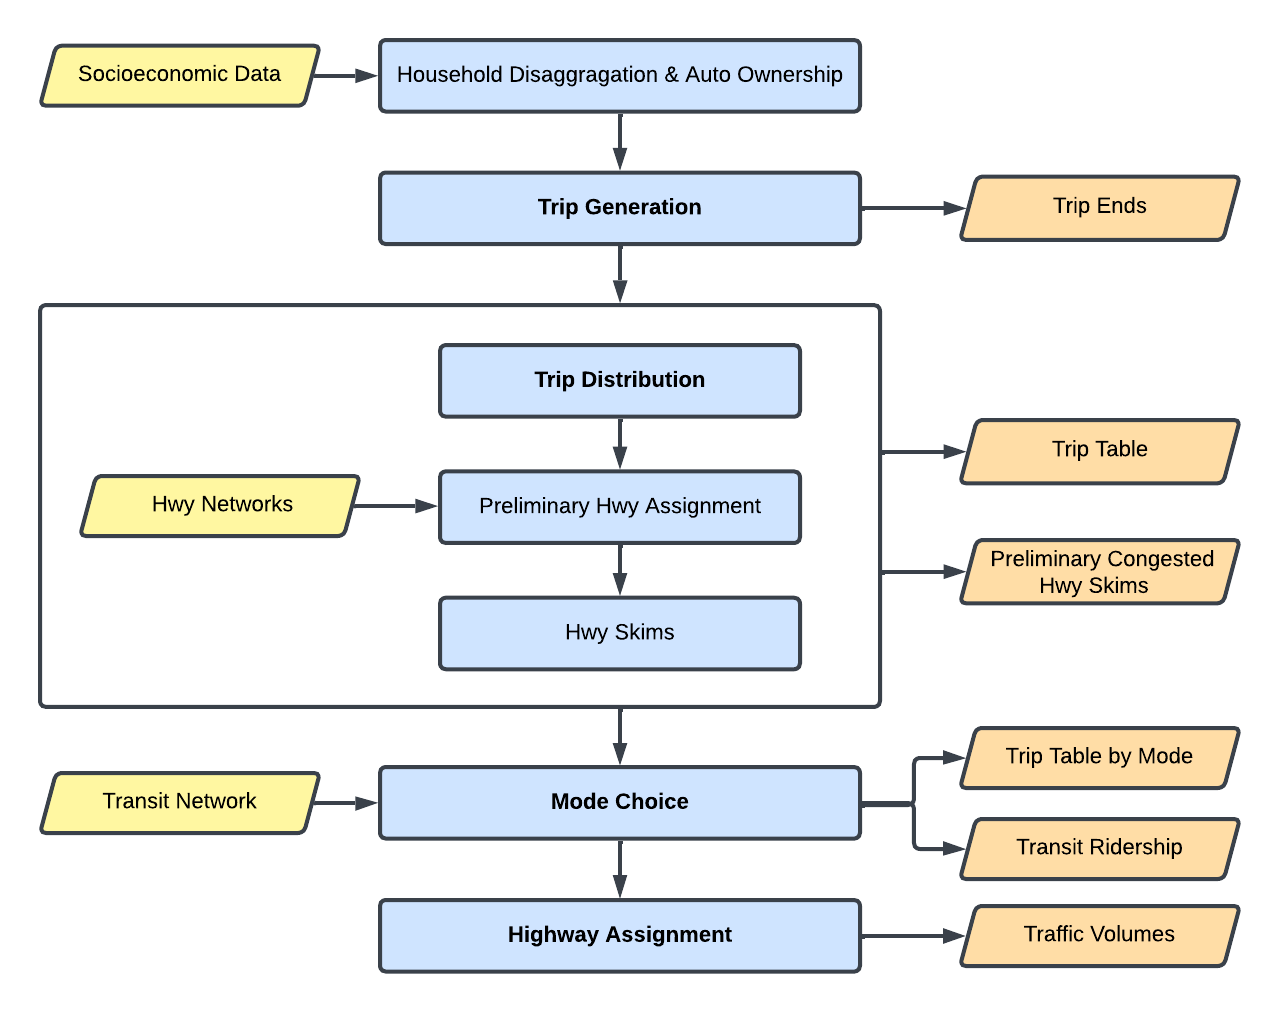
\includegraphics{qmd/./../images/wfrc_flowchart.png}

}

\caption[WFRC model flowchart.]{\label{fig-wfrc-flowchart}WFRC model
flowchart. Note the feedback loop in the distribution step where
preliminary loaded network skims are used to perform subsequent
iterations of trip distribution until the distribution converges.}

\end{figure}%

The disaggregation step takes TAZ-level socioeconomic data (such as
population, number of households, and average income) and estimates the
number of households belonging to each category of household size,
number of workers, income group, and vehicle ownership. The categories
of household size, number of workers, and vehicle ownership are
``capped'' at 6, 3, and 3, respectively, i.e.~every household with 3 or
more workers is grouped into a ``3+ workers'' category. The specific
income groups used in the WFRC model are given in
Table~\ref{tbl-income-groups}.

\begin{table}

\caption{\label{tbl-income-groups}Income Groups in the WFRC Model}

\centering{

\centering
\resizebox{\ifdim\width>\linewidth\linewidth\else\width\fi}{!}{
\begin{tabular}[t]{cc}
\toprule
Income Group & Income Range\\
\midrule
1 & ≤ \$45,000\\
2 & \$45,000–\$75,000\\
3 & \$75,000–\$125,000\\
4 & ≥ \$125,000\\
\bottomrule
\end{tabular}}

}

\end{table}%

There is an additional distribution estimated, which is termed ``life
cycle'' in the WFRC model. This distribution places households into one
of three categories, intended to represent the presence of children
and/or working adults in the household. This is done by estimating the
age distribution in each TAZ and categorizing each household based on
Table~\ref{tbl-lif-cyc-categories}.

\begin{table}

\caption{\label{tbl-lif-cyc-categories}Life Cycle Categories in the WFRC
Model}

\centering{

\centering
\resizebox{\ifdim\width>\linewidth\linewidth\else\width\fi}{!}{
\begin{tabular}[t]{c>{\centering\arraybackslash}p{.9in}>{\centering\arraybackslash}p{.9in}>{\centering\arraybackslash}p{.9in}}
\toprule
\multicolumn{1}{c}{ } & \multicolumn{3}{c}{Presence of persons in household aged:} \\
\cmidrule(l{3pt}r{3pt}){2-4}
Life Cycle & 0–18 & 18–64 & 65+\\
\midrule
1 & — & ✓ & —\\
2 & ✓ & ✓ & —\\
3 & ✓ & — & ✓\\
\bottomrule
\end{tabular}}

}

\end{table}%

The disaggregated household data is then used in the trip generation
step to estimate the number of trips produced from each TAZ. The trips
are estimated using lookup tables which assert an average number of
trips for each household type. There are separate lookup tables for each
trip purpose, and depending on the trip purpose the lookup table uses a
different household classification. The trip rates in the lookup tables
are multiplied by the number of households in each category, and this
gives a total number of trips by purpose produced in each TAZ.

The WFRC model contains the following trip purposes: Home-based Work,
Home-based Shopping, Home-based School, Home-based Other,
Non--home-based Work, and Non--home-based Non-work. The Home-based Work
and Non--home-based Work purposes use only the number of workers per
household in determining trip productions, and all other trip purposes
use the cross-classification of household size with life cycle.

Trip attractions are estimated for each purpose based mostly on the
number of jobs by industry in each TAZ. Home-based other and
non--home-based trip attractions also are affected by the number of
households in a TAZ, and school attractions are based on the school
enrollment by TAZ. Each purpose has a different coefficient for each
variable, and these are left unchanged from the existing values.

Trip distribution uses a gravity model of the form\\
\[
T_{ij} = P_i \times \frac{A_j  F_{ij}}{\displaystyle \sum_J A_j  F_{ij}},
\]\\
where \(T_{ij}\) is the number of trips from zone \(i\) to \(j\),
\(P_i\) is the productions at \(i\), \(A_j\) is the attractions at
\(j\), \(F_{ij}\) is the cost term/function from \(i\) to \(j\), and
\(J\) is the set of all zones trips from \(i\) can be attracted to.

The mode choice step uses a choice model to assign a percentage of trips
of each purpose to each mode, and network assignment is done via an
iterative process to equalize travel time between potential routes. The
WFRC model outputs include trip tables by purpose, mode, and time of
day, as well as loaded network skims.

\section{ActivitySim}\label{activitysim}

ActivitySim is an open-source ABM led by a consortium of transportation
planning agencies. ActivitySim is highly configurable, and many agencies
have their own bespoke implementation. This paper uses an ActivitySim
implementation based on the one used in Macfarlane and Lant (2021),
which is in turn based on the prototype configuration for the
Metropolitan Transportation Commission serving the San Francisco area
(Erhardt et al. 2011). The exact implementation is available on
GitHub.\footnote{
  {\href{https://github.com/byu-transpolab/wfrc_asim_scenario/tree/update-abm-illustration}{https://github.com\slash byu-transpolab\slash wfrc\_asim\_scenario\slash tree\slash update-abm-illustration}}}

ActivitySim requires similar inputs to the WFRC model, though it does
not assign traffic and so does not require any transportation networks.
However, ActivitySim does require network skims for information on
travel time, cost, etc. These skims are obtained from any network
assignment process, though ActivitySim itself does not include network
assignment. A discussion and comparison of network assignment processes
is outside the scope of this project, so this ActivitySim implementation
uses the travel skims output from the WFRC model directly. In practice,
ActivitySim is mated to CUBE or another network assignment algorithm for
network skimming and travel time feedback.

ActivitySim additionally requires population data at an individual
level, including information such as age, household income, and home
location. Due to privacy concerns, real data is rarely used for this
purpose, and a synthetic population representative of the study area is
used instead. Section~\ref{sec-populationsim} discusses the population
used in more detail.

ActivitySim, like all ABMs, simulates transportation decisions on an
individual level. ActivitySim has a hierarchical decision tree, where
long-term decisions (such as auto ownership and telecommute frequency)
are made first, followed by daily and tour- and trip-level decisions
such as scheduling and mode choice (see
Figure~\ref{fig-asim-flowchart}). Each of these steps determines
information that will be used in subsequent steps, and many steps can be
turned on or off depending on what is needed for the model
implementation.

\begin{figure}

\centering{

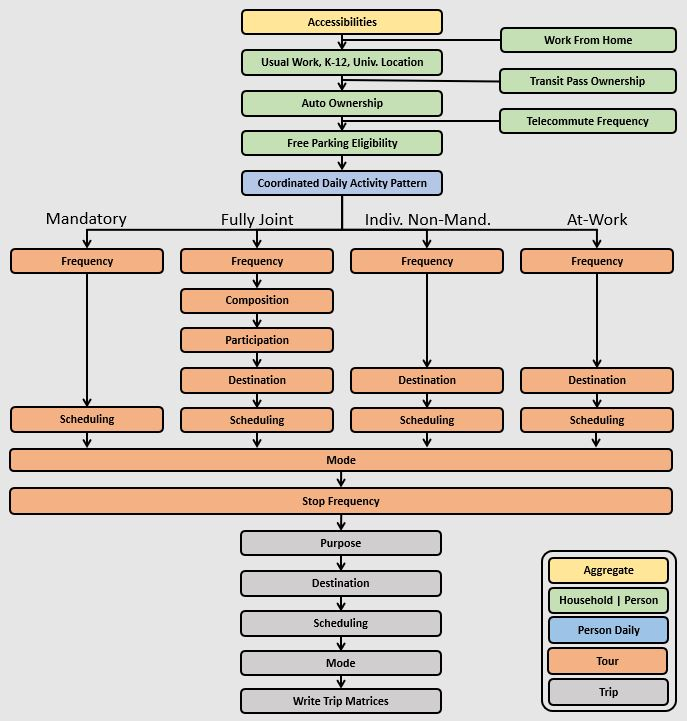
\includegraphics{qmd/../images/abmexample.jpg}

}

\caption[ActivitySim sub-model
flowchart.]{\label{fig-asim-flowchart}ActivitySim sub-model flowchart.
Long-term decisions are made first, followed by more granular ones.
Association of Metropolitan Planning Organizations (2022).}

\end{figure}%

The steps can broadly be categorized into five groups, as shown in
Figure~\ref{fig-asim-flowchart}: aggregate, household/personal, daily,
tour-level, and trip-level steps. The aggregate steps mainly involve
determining impedance measures between each pair of zones (travel time,
distance, cost, etc.). In this case, these impedances are supplied
directly as the network skims output from the WFRC model.

The household/personal steps relate to long-term decisions that are
unlikely to change quickly based on daily transportation conditions.
These steps include determining remote work status, work/school
location, auto ownership, transit pass ownership, and free parking
availability at work. Our ActivitySim implementation models remote work
status, work/school location, auto ownership, and free parking
availability, but transit pass ownership is not modeled and it is
assumed that everyone pays the transit fare.

The daily decisions primarily concern an individual's DAP. ActivitySim
contains a step to assign mandatory, non-mandatory, and home DAPs based
on personal and household information (a home DAP involves no travel).
For example, full-time workers are more likely to have a mandatory DAP
than part-time workers, all else being equal.

Once a DAP is chosen, ActivitySim creates tours for each major activity
in the day. Additionally, ActivitySim determines if an individual makes
an ``at-work'' tour (e.g.~leaving for lunch and returning to the
workplace). Each tour is scheduled and assigned a primary mode, as well
as a primary destination for non-mandatory and joint tours. The tours
are then populated with trips, and ActivitySim assigns each trip a
purpose, destination, time of day, and mode compatible with the
tour-level assignment.

The final steps of ActivitySim are writing output trip matrices and
other tables, including information on land use, persons, households,
tours, and trips.

Most of ActivitySim's individual models are based on a multinomial logit
model of the form:\\
\[
P(k) = \frac{e^{V_k}}{\displaystyle \sum_{k \in K} e^{V_k}},
\]\\
where \(P(k)\) is the probability of choosing alternative \(k\), \(V_k\)
is the utility of alternative \(k\), and \(K\) is the set of all
alternatives (as discussed in McFadden 1974). The utility values are
determined by coefficients on variables such as income, age, and work
status, in addition to calibration constants for each alternative.

\subsection{PopulationSim}\label{sec-populationsim}

This research uses PopulationSim (Association of Metropolitan Planning
Organizations 2023b) to create a synthetic population for ActivitySim.
The synthetic population aims to be representative of the study area
while maintaining privacy. Additionally, a synthetic population can be
adjusted in line with projected socioeconomic forecasts to perform
future-year analyses. PopulationSim takes as input a ``seed'' of
individuals and households, and populates the area with copies of these
to match given control totals.

The seed sample comes from the 2019 American Community Survey Public Use
Microdata Sample (U.S. Census Bureau 2022), which contains a sample of
actual (anonymized) individuals and households at the Public Use
Microdata Area (PUMA) geography (PUMAs partition the United States into
areas of around 100,000 people each (U.S. Census Bureau 2023)). The
control totals come from two different sources: the U.S. Census and the
WFRC model. Table~\ref{tbl-control-totals} shows these controls as well
as their geographic level and source. The geography of a control
dictates PopulationSim's ``level of precision'' in matching the control
totals. For example, with our configuration, PopulationSim will attempt
to match the average number of workers per household to the Census
average for each Census tract, while the total population is only
controlled for across the entire region. PopulationSim also allows
setting different weights to each control, and
Table~\ref{tbl-control-totals} gives this information as well. Because
the Public Use Microdata Sample does not contain every possible
combination of variable values, it is not possible to create a synthetic
population that perfectly matches every control total. The weights allow
certain controls to ``take priority'' over others; for example with this
configuration PopulationSim will prioritize the average household size
over the average number of workers per household if the two controls
cannot both be satisfied.

\begin{table}

\caption{\label{tbl-control-totals}PopulationSim Control Totals by
Geography and Source}

\centering{

\centering
\resizebox{\ifdim\width>\linewidth\linewidth\else\width\fi}{!}{
\begin{tabular}[t]{lllr}
\toprule
Control & Geography & Source & Weight\\
\midrule
Population & Entire Region & Census & 5,000\\
Number of Households & TAZ & WFRC Model & 1,000,000,000\\
Household Size & Census Tract & Census & 10,000\\
Persons by Age Group & Census Tract & Census & 10,000\\
Households by Income Group & Census Tract & Census & 500\\
Workers per Household & Census Tract & Census & 1,000\\
\bottomrule
\end{tabular}}

}

\end{table}%

Most of these controls come from Census data, with only the number of
households per TAZ coming from the WFRC model data. Note also that there
are many personal and household variables that are not accounted for in
these controls, such as sex, vehicle ownership, internet access, etc.
These variables are not controlled for and are dependent on which seed
persons or households are copied in controlling for the other variables.
However, this process is assumed to still give a representative enough
estimate for the uncontrolled variables without needing to model them
explicitly.

The outputs of PopulationSim include a persons and households table
comprising the synthetic population.

\section{Initial Model
Comparison/Calibration}\label{initial-model-comparisoncalibration}

While this research generally does not directly compare the outputs of
ActivitySim to those of the WFRC model, it is important to ensure
similar performance between the two models for meaningful analyses. As
such, a baseline scenario in both models is used in order to calibrate
the ActivitySim implementation to the WFRC model. This baseline scenario
uses the 2019 WFRC model as-is. For ActivitySim, the baseline scenario
uses 2019 Census and WFRC data to create the synthetic population, and
uses land use data and network skims from the baseline WFRC scenario for
accessibility and socioeconomic measures.

\subsection{Validation of the Synthetic
Population}\label{validation-of-the-synthetic-population}

The controls for PopulationSim mostly come from the Census, as can be
seen in Table~\ref{tbl-control-totals}. However, the WFRC model contains
TAZ-level data including population and median income. The WFRC model
also has a disaggregation step that estimates the number of households
by size and income group. This section compares the output of
PopulationSim to the WFRC model on each of these variables. Though these
outputs are given at the TAZ level, most controls to PopulationSim were
given at the Census tract level, and these tracts are not a one-to-one
match with the region's TAZs. Because of this, PopulationSim has some
amount of randomness in which TAZ it places each household in, and so at
small geographies such as TAZs the error distribution between the two
models is noisy. The comparisons in this section are therefore made by
aggregating each TAZ at the district level.

Figure~\ref{fig-population-comparison} shows the difference in district
population between PopulationSim and the WFRC data. It is worth noting
that since the number of households was controlled at the TAZ level from
the WFRC data with an extremely high weight, the number of households
per TAZ in the synthetic population match exactly to the WFRC data. The
average household size will therefore follow a similar error
distribution to the one shown in Figure~\ref{fig-population-comparison}.

\begin{figure}

\centering{

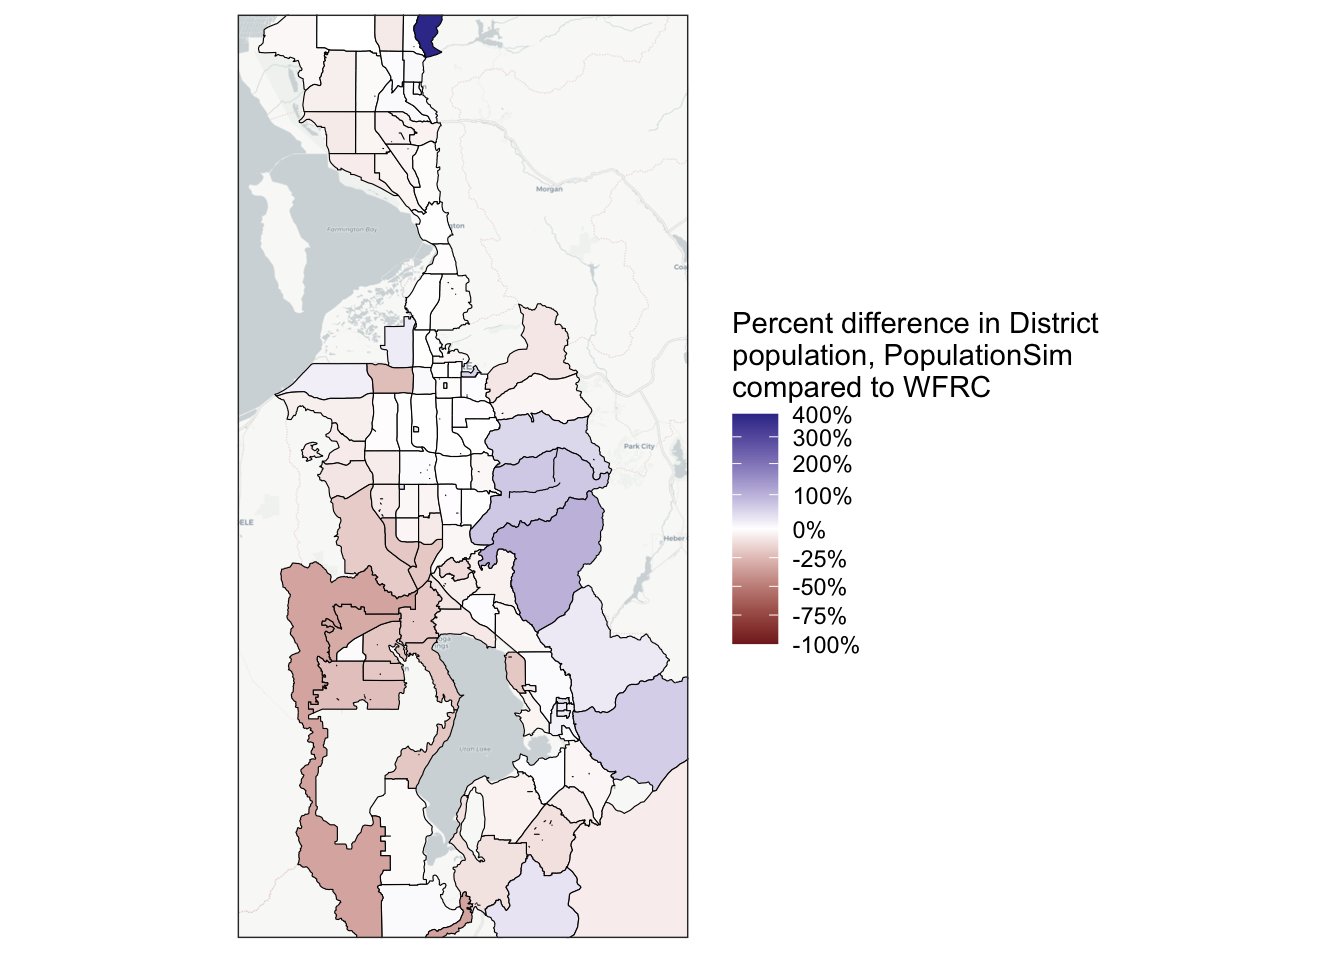
\includegraphics{qmd/methods_files/figure-pdf/fig-population-comparison-1.png}

}

\caption{\label{fig-population-comparison}Population by district,
PopulationSim compared to the TAZ-level socioeconomic data in the WFRC
Model.}

\end{figure}%

The population per district is similar to the WFRC data in most places,
though there are some discrepancies especially near Herriman and Lehi.
Since total population is a region-level control, but number of
households is a TAZ-level control, this shows PopulationSim is
predicting a smaller average household size in Herriman and Lehi than
the WFRC data suggests.

Income is also an important factor in travel behavior (Zegras and
Srinivasan 2007), and Figure~\ref{fig-median-income-comparison} shows a
district-level comparison of median income between the synthetic
population and the WFRC data. The synthetic population does have a lower
median income than the WFRC data in many districts, but the error is in
most cases fairly small, especially in more populated areas.

\begin{figure}

\centering{

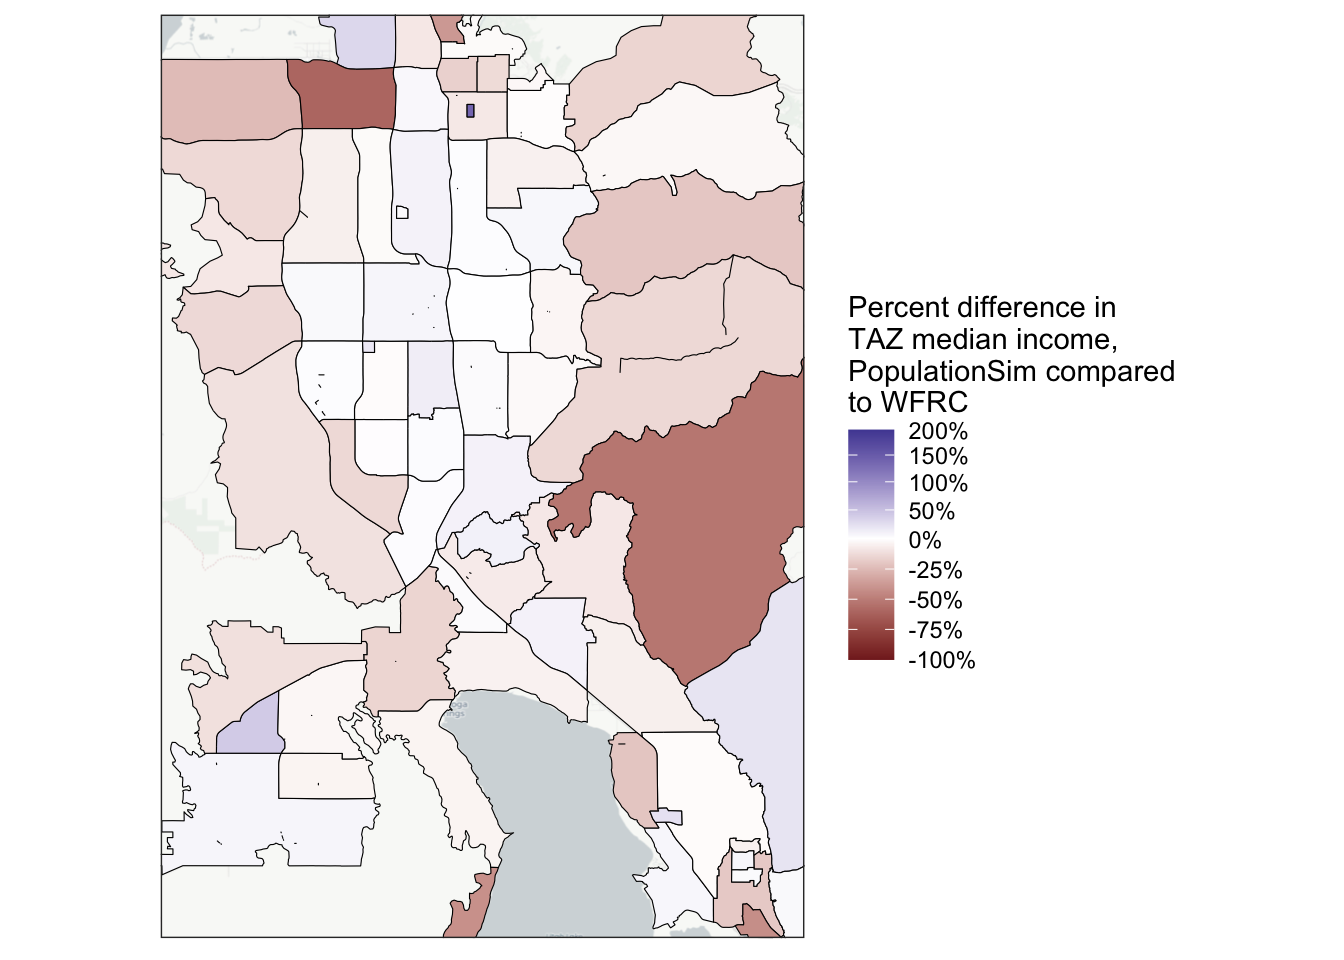
\includegraphics{qmd/methods_files/figure-pdf/fig-median-income-comparison-1.png}

}

\caption{\label{fig-median-income-comparison}District-level median
income, PopulationSim compared to the TAZ-level socioeconomic data in
the WFRC Model.}

\end{figure}%

However, both the WFRC model and ActivitySim use household income
\emph{groups} rather than individual household income to inform travel
decisions. These groups are taken from the WFRC model (see
Table~\ref{tbl-income-groups}), and the groups in PopulationSim and
ActivitySim were adjusted to match. Figure~\ref{fig-income-group-map}
shows the difference in number of households by income group. This
figure shows PopulationSim predicting slightly more high-income
households, though the error for the lower three groups is more evenly
distributed, especially in more populated areas.

\begin{sidewaysfigure}[p]

\centering{

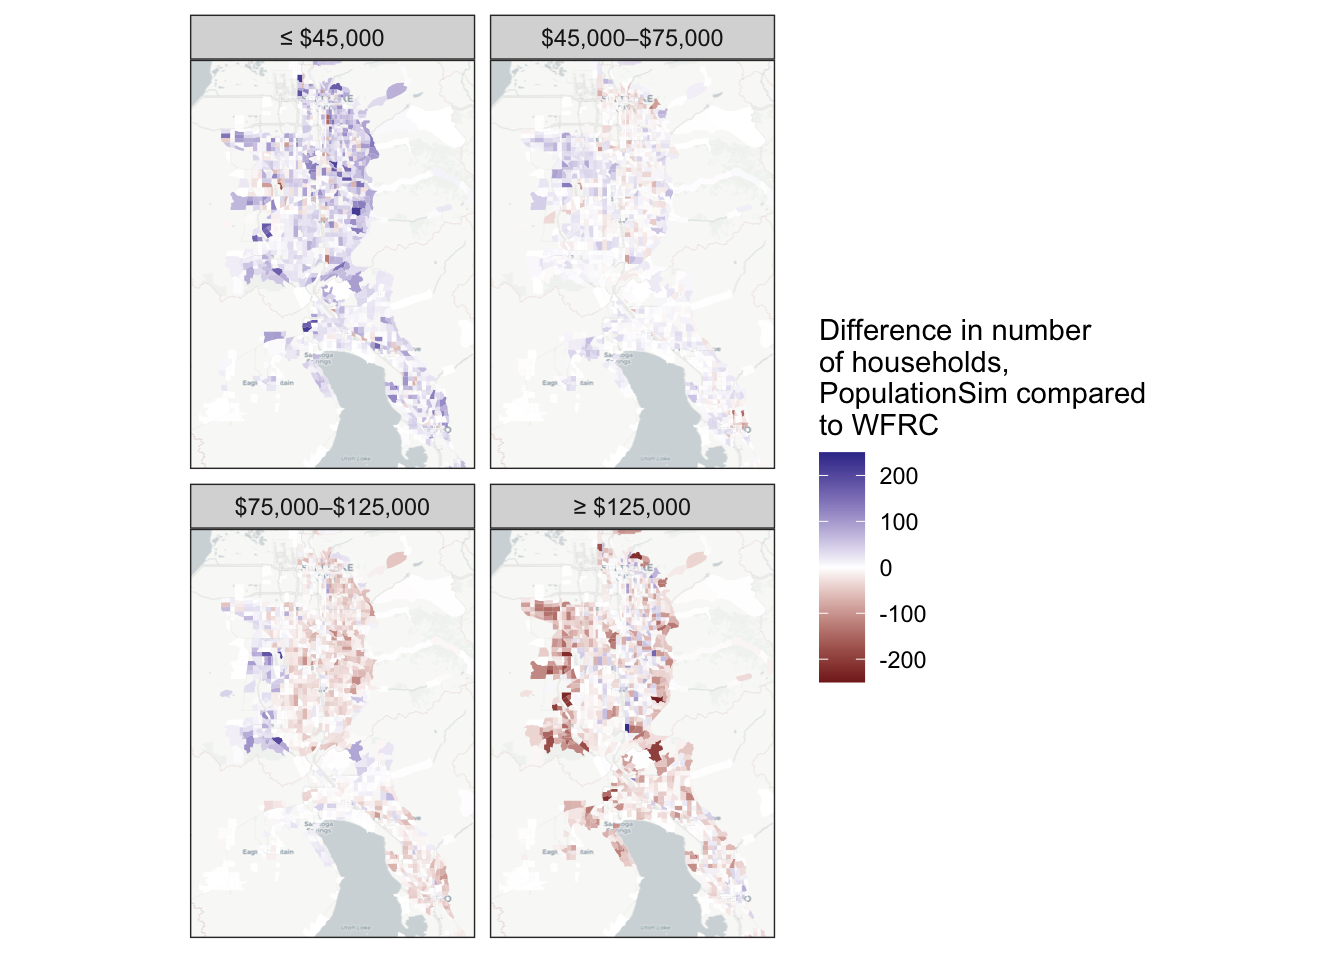
\includegraphics{qmd/methods_files/figure-pdf/fig-income-group-map-1.png}

}

\caption{\label{fig-income-group-map}Households in each income group,
PopulationSim compared to the TAZ-level socioeconomic data in the WFRC
Model.}

\end{sidewaysfigure}%

Note that in the synthetic population, each household has a specific
income and so can be grouped directly, while the WFRC model requires a
disaggregation step to estimate the number of households in each income
group. Figure~\ref{fig-income-group-map} therefore is comparing two
income disaggregation models, one a part of PopulationSim and the other
in the WFRC model, rather than comparing the synthetic population to
actual socioeconomic data. With this in mind, the difference shown in
Figure~\ref{fig-income-group-map} is within an acceptable margin of
error.

Additionally, the overall distribution of income is similar between the
models, as Figure~\ref{fig-median-income-density} shows. A
production-ready synthetic population would match its income
distribution more closely to the existing WFRC model, but for the
purposes of this research the income distribution of the synthetic
population is acceptable.

\begin{figure}

\centering{

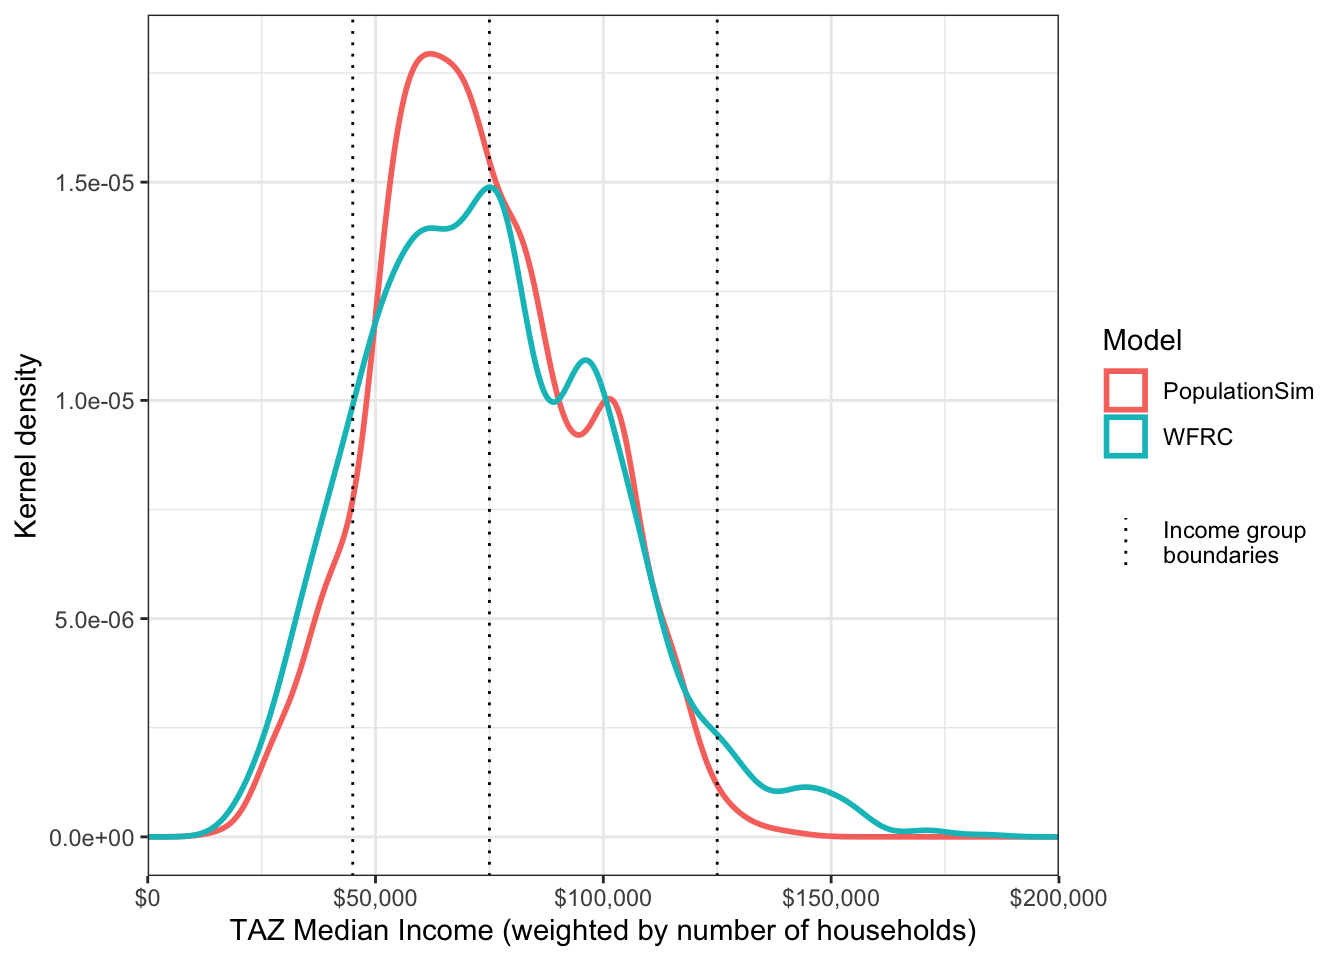
\includegraphics{qmd/methods_files/figure-pdf/fig-median-income-density-1.png}

}

\caption{\label{fig-median-income-density}Distribution of TAZ median
income, PopulationSim compared to the TAZ-level socioeconomic data in
the WFRC Model.}

\end{figure}%

\subsection{Validation and Calibration of
ActivitySim}\label{sec-baseline-calibration}

This section compares the outputs of both models to verify that trip
patterns roughly agree between them. There are three comparisons of
interest that we make between the outputs of the two models: mode split,
trip length frequency distribution, and remote work.

The initial baseline ActivitySim scenario predicted a mode split
significantly different to that from the WFRC model, and so calibration
efforts were needed. The ideal approach would be to calibrate the mode
choice model to recent travel survey data, such as from the Utah
Household Travel Survey. However, recent travel survey data was not
available for this project, and only a rough calibration is needed for
the purposes of this research. We therefore used the outputs of the
baseline WFRC model scenario as mode split targets. A production model
would certainly use travel survey data and perform a thorough
calibration, but that is outside the scope of this project.

Before beginning calibration, we created a crosswalk between the
available modes in ActivitySim and in the WFRC model. The available
modes between ActivitySim and the WFRC model are not incredibly
different, and in fact many modes have a 1-to-1 match between the
models. However, some adjustment was needed, and
Table~\ref{tbl-mode-crosswalk} shows the adjustments that were made.

ActivitySim additionally has ridehail modes, but the WFRC model does
not, and so there are no obvious calibration targets for ridehail. Based
largely on the model results of Day (2022), and partly on the existing
(uncalibrated) mode split in ActivitySim, we asserted the following mode
shares for ridehail: 0.015\% for Home-based Work trips, 0.38\% for
Home-based Other trips, and 0.4\% for Non--home-based trips.

\begin{table}

\caption{\label{tbl-mode-crosswalk}Crosswalk Between Modes in Both
Models}

\centering{

\centering
\resizebox{\ifdim\width>\linewidth\linewidth\else\width\fi}{!}{
\begin{tabular}[t]{>{\raggedright\arraybackslash}m{1.2in}>{\raggedright\arraybackslash}m{1.4in}>{\raggedright\arraybackslash}m{1.9in}}
\toprule
Calibration Mode & WFRC Mode(s) & ActivitySim Mode(s)\\
\midrule
Drive Alone & DA & DRIVEALONEFREE\\
Carpool (2) & SR2 & SHARED2FREE\\
Carpool (3+) & SR3p & SHARED3FREE\\
Walk & walk & WALK\\
Bike & bike & BIKE\\
Local Bus & dBRT, dCOR, dLCL, wBRT, wCOR, wLCL & WALK\_LOC, DRIVE\_LOC\\
Commuter Rail & dCRT, wCRT & WALK\_HVY, WALK\_COM, DRIVE\_HVY, DRIVE\_COM\\
Express Bus & dEXP, wEXP & WALK\_EXP, DRIVE\_EXP\\
Light Rail & dLRT, wLRT & WALK\_LRF, DRIVE\_LRF\\
\bottomrule
\end{tabular}}

}

\end{table}%

Additionally, since the WFRC model has a significantly different mode
split depending on the trip purpose, we calibrated each trip purpose
individually. However, a crosswalk of trip purposes between the models
is more complicated than the crosswalk for modes. Because ABMs create
tours first, which are then populated with trips, an ABM's idea of
``trip purpose'' is entirely different to that of a trip-based model.
Specifically, an ABM doesn't have a concept of e.g.~``home-based work''
trips, there are simply trips on a ``work'' tour, some of which have an
origin or destination at home. For simplicity, though, we converted the
trips from ActivitySim into purposes that roughly match the WFRC model's
purposes. Any trip that doesn't start or end at home is considered a
Non--home-based trip, and if a trip starting or ending at home has its
other end at work, it is considered a Home-based Work trip. All other
trips are considered Home-based Other trips.

To perform the calibration, the output mode split of ActivitySim for
each purpose was compared to the target mode split output from the WFRC
model. An adjustment value was determined by the formula
\(A_k = \ln(T_k/M_k)\), where \(A_k\) is the adjustment value for mode
\(k\), \(T_k\) is the target mode share of mode \(k\), and \(M_k\) is
the ActivitySim-predicted mode share of mode \(k\). This adjustment
value was added to the current alternative-specific constants (ASCs) in
the ActivitySim configuration, and this process was repeated iteratively
until calibration was satisfactory.

There are two aspects of this calibration process worth noting. The
first is that ActivitySim contains ASCs for both tour mode choice and
trip mode choice, where the tour mode is the principal mode used on the
tour, and the trip mode is the mode of the individual trip (for example,
there could be a ``walk'' trip on a ``transit'' tour). Because
tour-level mode choice influences trip mode choice, both the tour-level
and trip-level ASCs were adjusted by the calculated adjustment value for
each mode. The second is that while it is possible to categorize
ActivitySim trips into purposes similar to a trip-based model,
ActivitySim does not do this conversion internally. ActivitySim
\emph{does} have separate ASCs by purpose, but these purposes are
ActivitySim's tour purposes, rather than purposes resembling those in a
trip-based model. Though it is not a perfect correspondence to how the
adjustment values were calculated, we adjusted the ASCs as follows: All
ActivitySim ``atwork'' ASCs are calibrated with the Non--home-based
adjustment, all ``work'' ASCs are calibrated with the Home-based Work
adjustment, and all other ASCs are calibrated with the Home-based Other
adjustment.

Figure~\ref{fig-mcc-adjustments} shows the mode split from ActivitySim
compared against the target mode split for each iteration of
calibration. After a few iterations, the mode split more closely matches
between the models; however, there are still some discrepancies.
ActivitySim has mode choice ASCs separated not only by mode and purpose,
but also by many personal variables, such as income, age, and vehicle
ownership. The difference across these categories was left unchanged,
and all ASCs for a given mode and purpose were adjusted equally. Our
ActivitySim configuration is ultimately based on the San Francisco area,
and so coefficients on variables such as travel time and income are
calibrated for that area. Additionally, we did not calibrate the vehicle
ownership model, and this may be partly the cause of the discrepancies.

\begin{sidewaysfigure}[p]

\centering{

\includegraphics{qmd/methods_files/figure-pdf/fig-mcc-adjustments-1.png}

}

\caption{\label{fig-mcc-adjustments}Mode choice calibration, target
vs.~actual shares over several iterations.}

\end{sidewaysfigure}%

In any case, we chose the calibration at Iteration 4 for the final ASC
values, as subsequent iterations adjusted the ASCs without changing the
mode split very much. At subsequent iterations ActivitySim was also less
sensitive to changes in infrastructure due to over-calibration, which
would not allow for effective policy analysis.
Table~\ref{tbl-mode-split} compares the mode split of both models after
iteration 4 of calibration. Overall, the calibration resulted in a
reasonably similar mode split between the two models, though there are
still discrepancies (e.g.~ActivitySim is predicting significantly more
transit trips compared to the WFRC model). While the calibration is not
perfect, for the purposes of this research this calibration is
reasonable enough.

\begin{table}

\caption{\label{tbl-mode-split}Comparison of Mode Split Between Models
After Calibration}

\centering{

\centering
\resizebox{\ifdim\width>\linewidth\linewidth\else\width\fi}{!}{
\begin{threeparttable}
\begin{tabular}[t]{cccccc}
\toprule
\multicolumn{2}{c}{ } & \multicolumn{2}{c}{ActivitySim} & \multicolumn{2}{c}{WFRC Model} \\
\cmidrule(l{3pt}r{3pt}){3-4} \cmidrule(l{3pt}r{3pt}){5-6}
Purpose & Mode & Trips & Share & Trips & Share\\
\midrule
 & Drive Alone & 1012180 & 60.6\% & 1328609 & 77.6\%\\

 & Carpool & 258459 & 15.5\% & 257783 & 15.1\%\\

 & Bus & 171875 & 10.3\% & 18870 & 1.1\%\\

 & Rail & 80193 & 4.8\% & 29847 & 1.7\%\\

 & Ridehail & 1108 & 0.1\% & — & —¹\\

\multirow{-6}{*}{\centering\arraybackslash Home-based Work} & Non-motorized & 145957 & 8.7\% & 76505 & 4.5\%\\
\cmidrule{1-6}
 & Drive Alone & 702594 & 18.2\% & 1394415 & 30.0\%\\

 & Carpool & 2154115 & 55.8\% & 2702277 & 58.2\%\\

 & Bus & 149217 & 3.9\% & 17717 & 0.4\%\\

 & Rail & 127969 & 3.3\% & 19591 & 0.4\%\\

 & Ridehail & 114278 & 3.0\% & — & —¹\\

\multirow{-6}{*}{\centering\arraybackslash Home-based Other} & Non-motorized & 614901 & 15.9\% & 510144 & 11.0\%\\
\cmidrule{1-6}
 & Drive Alone & 716885 & 36.3\% & 951561 & 39.9\%\\

 & Carpool & 939668 & 47.6\% & 1273279 & 53.4\%\\

 & Bus & 99000 & 5.0\% & 4888 & 0.2\%\\

 & Rail & 21010 & 1.1\% & 8538 & 0.4\%\\

 & Ridehail & 40283 & 2.0\% & — & —¹\\

\multirow{-6}{*}{\centering\arraybackslash Non–home-based} & Non-motorized & 157006 & 8.0\% & 146404 & 6.1\%\\
\bottomrule
\end{tabular}
\begin{tablenotes}
\item[1] Ridehail mode shares were asserted for mode choice calibration, but are not counted here
\end{tablenotes}
\end{threeparttable}}

}

\end{table}%

Figure~\ref{fig-tlfd-comp} compares the trip length frequency
distribution of the two models by mode and purpose. Both ActivitySim and
the WFRC model contain trip distribution steps which can be adjusted to
affect the distribution of trip length. However, as the figure shows,
the two models have similar trip length frequency distributions, so no
adjustment was necessary. The most significant discrepancies are with
transit trips, again likely due to this configuration of ActivitySim
being developed for San Francisco, making transit more attractive. Note
that though these distributions match well enough for the purposes of
this research, further calibration would be required to create a
production-ready ActivitySim implementation.

\begin{figure}

\centering{

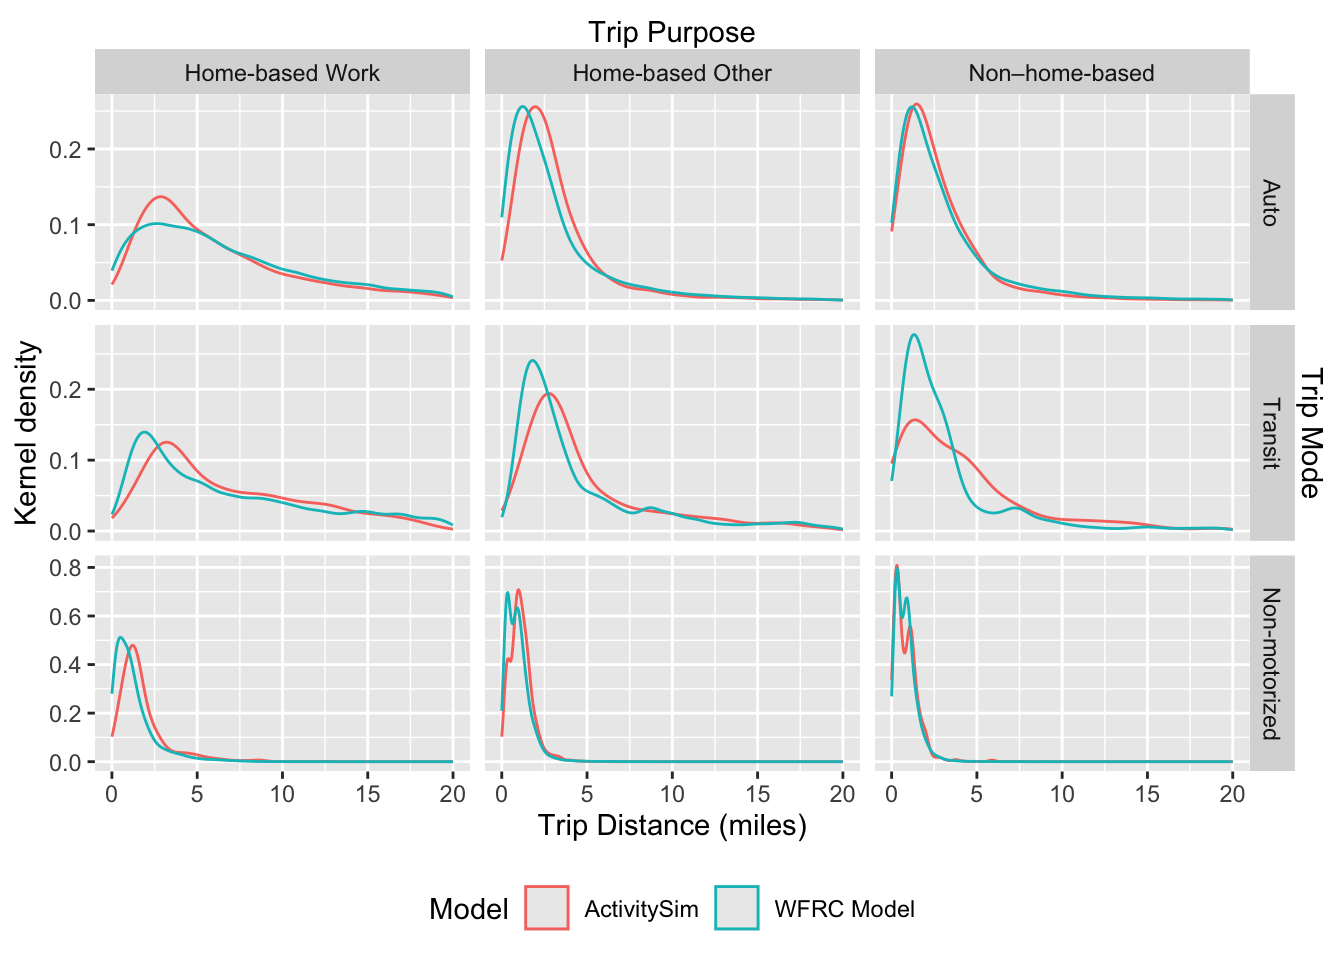
\includegraphics{qmd/methods_files/figure-pdf/fig-tlfd-comp-1.png}

}

\caption{\label{fig-tlfd-comp}Comparison between models of trip length
frequency distribution.}

\end{figure}%

The WFRC model has basic support for predicting telecommuting and
work-from-home trips. This includes a lookup table of telecommute
percentages based on job type and year. ActivitySim also has this
functionality, and can additionally use individual- and household-level
variables in its predictions. It is worth noting that both the WFRC
model and ActivitySim make a distinction between ``telecommuting'',
where an individual commutes to work some days and does not others, and
``work-from-home'' (called ``home-based jobs'' in the WFRC model), where
an individual's workplace is always at their home.

The ActivitySim implementation discussed in Macfarlane and Lant (2021)
does not include any submodels related to remote work. However, a
separate ActivitySim implementation, developed for the Southeast
Michigan Council of Governments (SEMCOG) metropolitan planning
organization in Michigan, \emph{does} include these submodels, and our
ActivitySim implementation takes these submodels directly from the
SEMCOG implementation. Some modifications to the remote work submodels
were needed for compatibility, but these modifications were minor and
mostly involved ensuring the variable names from the SEMCOG submodels
were consistent with the existing implementation.

Both models treat ``work-from-home''/``home-based jobs'' similarly. The
WFRC model's land use data contains employment by type in each TAZ, and
it considers a ``home-based job'' as a separate job type, so these are
not counted toward employment totals in trip generation and subsequent
steps. ActivitySim has a ``work from home'' submodel which assigns
workers work-from-home status based on personal variables such as
income, sex, and education (coefficients on these variables were left
unchanged from the existing configuration, see
Table~\ref{tbl-asim-wfh-model-coeffs}). There is also a ``target
work-from-home percent'' value that adjusts the model to reach the
specified work-from-home proportion of all workers. Individuals with
work-from-home status are then prohibited from making a mandatory tour.
This target work-from-home percentage is set at 2.3\%, based on a
weighted average from the WFRC model data. We made no other adjustments
to the ActivitySim work-from-home submodel.

\begin{table}

\caption{\label{tbl-asim-wfh-model-coeffs}Work-From-Home Submodel
Coefficients in ActivitySim}

\centering{

\centering
\resizebox{\ifdim\width>\linewidth\linewidth\else\width\fi}{!}{
\begin{tabular}[t]{lc}
\toprule
Description & Coefficient\\
\midrule
Constant for Working from home & 0.438\\
Full time worker (1 if true) & -0.812\\
Female Worker & -0.347\\
Female worker with a Preschool Child in Household & 0.573\\
Accessibility to workplaces of the home mgra & -0.140\\
Presence of Non Working Adult in the Household & -0.372\\
Education Level Bachelors or higher degree & 0.285\\
Household income Less than 30K & -0.393\\
Age Group - Less than 35 years & -0.574\\
Age Group - 35 yrs to 45 yrs & 0.000\\
Age Group - 45 yrs to 55 yrs & 0.214\\
Age Group - 55 yrs to 65 yrs & 0.452\\
Age Group - Older than 65yrs & 0.584\\
\bottomrule
\end{tabular}}

}

\end{table}%

The two models differ in their approach to telecommuting, however. The
WFRC model has a lookup table of telecommuting shares based on job type
(see Table~\ref{tbl-baseline-telecommute}), including predictions for
future years. ActivitySim has a ``telecommute frequency'' submodel which
assigns workers a telecommute status indicating the number of days they
work remotely per week. Based on this status, ActivitySim adjusts the
likelihood of selecting a mandatory DAP. Telecommute status depends on
personal variables similar to those in the work-from-home submodel by
default. Notably, the telecommute frequency submodel also includes
adjustments based on an individual's distance to work. No other changes
were made to the existing variables in this submodel, and
Table~\ref{tbl-asim-tc-model-coeffs} shows the submodel coefficients.

\begin{table}

\caption{\label{tbl-asim-tc-model-coeffs}Telecommute Frequency Submodel
Coefficients in ActivitySim}

\centering{

\centering
\resizebox{\ifdim\width>\linewidth\linewidth\else\width\fi}{!}{
\begin{tabular}[t]{l>{\centering\arraybackslash}p{0.87in}>{\centering\arraybackslash}p{0.87in}>{\centering\arraybackslash}p{0.87in}}
\toprule
\multicolumn{1}{c}{ } & \multicolumn{3}{c}{Telecommute Frequency Coefficients} \\
\cmidrule(l{3pt}r{3pt}){2-4}
Description & 1 day & 2–3 days & 4 days\\
\midrule
Has children 0 to 5 years old & 0.000 & 0.000 & -0.864\\
Has children 6 to 12 years old & 0.000 & 0.517 & -0.810\\
One adult in hh & 0.177 & 0.000 & -0.043\\
Part-time worker & 0.000 & 0.425 & 1.112\\
College student & 0.000 & 0.600 & 0.000\\
Pays to park & 0.457 & 0.000 & 0.000\\
Income 60-100k & 0.560 & 0.389 & 0.000\\
Income 100-150k & 0.644 & 0.193 & 0.000\\
Income 150k+ & 0.920 & 0.765 & 0.000\\
0 autos & 0.000 & 0.407 & 0.000\\
3+ autos & 0.000 & -0.730 & 0.000\\
Distance to work & 0.016 & 0.000 & 0.000\\
\bottomrule
\end{tabular}}

}

\end{table}%

In order to calibrate ActivitySim's telecommute frequency submodel to
the WFRC data, however, we added additional job type variables to
ActivitySim to match those given in
Table~\ref{tbl-baseline-telecommute}. Because these are choice
coefficients rather than target percentages, the values needed to be
calibrated to match the WFRC targets. The calibration allowed
ActivitySim to match these targets exactly, and the coefficients are
given in Table~\ref{tbl-baseline-telecommute}.

\begin{table}

\caption{\label{tbl-baseline-telecommute}Telecommute Rates and
Coefficients by Job Industry}

\centering{

\centering
\resizebox{\ifdim\width>\linewidth\linewidth\else\width\fi}{!}{
\begin{tabular}[t]{l>{\centering\arraybackslash}p{1.3in}>{\centering\arraybackslash}p{0.87in}>{\centering\arraybackslash}p{0.87in}>{\centering\arraybackslash}p{0.87in}}
\toprule
\multicolumn{2}{c}{ } & \multicolumn{3}{c}{Telecommute Frequency Coefficients} \\
\cmidrule(l{3pt}r{3pt}){3-5}
Industry & 2019 WFRC Telecommute \% & 1 day & 2–3 days & 4 days\\
\midrule
Retail & 2.70\% & 0.312 & 0.125 & 0.078\\
Food & 1.87\% & -0.368 & -0.148 & -0.092\\
Manufacturing & 2.02\% & 0.038 & 0.015 & 0.010\\
Office & 6.66\% & 1.782 & 0.712 & 0.445\\
Gov't/Education & 1.67\% & -0.560 & -0.224 & -0.140\\
Health & 2.86\% & 0.158 & 0.063 & 0.039\\
Agriculture & 6.93\% & 2.262 & 0.904 & 0.566\\
Mining & 0.53\% & -2.030 & -0.810 & -0.511\\
Construction & 3.28\% & 0.816 & 0.326 & 0.204\\
Other & 5.37\% & 1.535 & 0.614 & 0.384\\
\bottomrule
\end{tabular}}

}

\end{table}%

Because both remote work submodels in ActivitySim are run before an
individual's DAP is chosen, ActivitySim can model a ``rebound effect'',
where individuals working remotely on any given day may be more likely
to make discretionary tours. However, because the WFRC model does not
include this effect, the ActivitySim DAP model is left unchanged.
Table~\ref{tbl-asim-dap-model-rw-coeffs} shows the coefficients of the
DAP model for individuals who work remotely.

\begin{table}

\caption{\label{tbl-asim-dap-model-rw-coeffs}Daily Activity Pattern
Submodel Coefficients in ActivitySim}

\centering{

\centering
\resizebox{\ifdim\width>\linewidth\linewidth\else\width\fi}{!}{
\begin{tabular}[t]{lccc}
\toprule
Status & Mandatory DAP & Non-mandatory DAP & Home DAP\\
\midrule
Telecommutes 1 day per week & 0 & 0.526 & 0.496\\
Telecommutes 2-3 days per week & 0 & 1.387 & 1.584\\
Telecommutes 4 days per week & 0 & 1.848 & 1.711\\
Full time worker, works from home & -999 & 0.000 & 0.000\\
Part time worker, works from home & -999 & 0.000 & 0.000\\
\bottomrule
\end{tabular}}

}

\end{table}%

\section{Example Scenarios}\label{example-scenarios}

With these two calibrated models, we created three model scenarios to
implement and run in each model for comparison. This is not a
comprehensive list covering all potential scenario possibilities, but
the scenarios identified here are intended to represent the main goals
of travel demand modeling in modeling changes in travel behavior. Change
in travel behavior could arise in response to changes in land use,
transportation infrastructure, and social/economic factors, and so we
create three hypothetical model scenarios that each implement one of
these aspects.

The first scenario involves a change in land use near the former state
prison site in Draper, Utah. Current plans for this site involve new
development known as ``The Point'', which will add high-density housing
and commercial development to the area. This research scenario will be
based on this development, but will include only the land use changes.
The actual development plans also include expansion of transit, but this
will not be a part of this scenario.

The second scenario centers around a change in transportation
infrastructure, namely an augmentation of commuter rail service along
the Wasatch Front. The FrontRunner, a commuter rail line connecting
Provo to Ogden, is slated for expansion. The expansion includes
additional stations and increased travel speeds due to vehicle
electrification. This scenario models these changes in accordance with
the planned expansion of the service.

The third scenario addresses the growing trend of remote work. Given
technological advancements and the notable surge in remote work during
the COVID-19 pandemic, this scenario models a substantial increase in
remote work based on projections from WFRC.

Each of these scenarios is based on the baseline 2019 scenario in the
respective model, and ignores any additional expected growth or
development beyond the specific changes of each scenario. For example,
the increased WFH scenario uses WFH projections from 2050, but land use
and socioeconomic data from 2019. These scenarios are therefore not
realistic, but they serve as illustrative examples of the types of
planning and development scenarios agencies may wish to analyze.

All three of these scenarios are coded in both the WFRC model and
ActivitySim. The results (Chapters \ref{sec-landuse}--\ref{sec-wfh})
describe the process of coding each scenario and analyzing them, as well
as the analyses themselves.

\bookmarksetup{startatroot}

\chapter{Scenario 1: Change in Land Use}\label{sec-landuse}

One of the primary ways that travel behavior is affected is through
changes in land use. Such changes involve the addition or removal of
households and/or jobs in an area, and our first model scenario, termed
the ``Land Use'' scenario, addresses this aspect of travel demand
modeling by simulating a new development in a single area. The basis for
the Land Use scenario is the redevelopment of a defunct prison site near
Draper, Utah. This redevelopment is part of the actual plan for the
area, and the new development is known as The Point (Point of the
Mountain State Land Authority and Skidmore, Owings \& Merril 2021).

This scenario models the change in transportation behavior that a
development such as The Point would create. Though the actual
development plans for The Point include an expansion of transit services
(Point of the Mountain State Land Authority and Skidmore, Owings \&
Merril 2021), only the additional households and jobs created from this
development are represented in this scenario. The data for the land use
changes comes from the WFRC land use forecast, which is in turn based on
projections from the Point of the Mountain State Land Authority (State
Land Authority 2021). The Point development is expected to be fully
completed by 2050, and its projected land use and socioeconomic data is
included in the 2050 WFRC forecast, so the 2050 WFRC land use and
socioeconomic data projections are used for this site.

The site consists of 5 TAZs, as shown in
Figure~\ref{fig-the-point-zones}. Table~\ref{tbl-the-point-data-old}
shows the households, population, and employment by type of these TAZs
in the baseline scenario, and Table~\ref{tbl-the-point-data-new} shows
this information with the new land use. Notably, there were no
households and relatively few jobs in these TAZs in the baseline
scenario. No changes other than to the land use/socioeconomic data in
these 5 TAZs were made relative to the baseline scenario.

\begin{figure}

\centering{

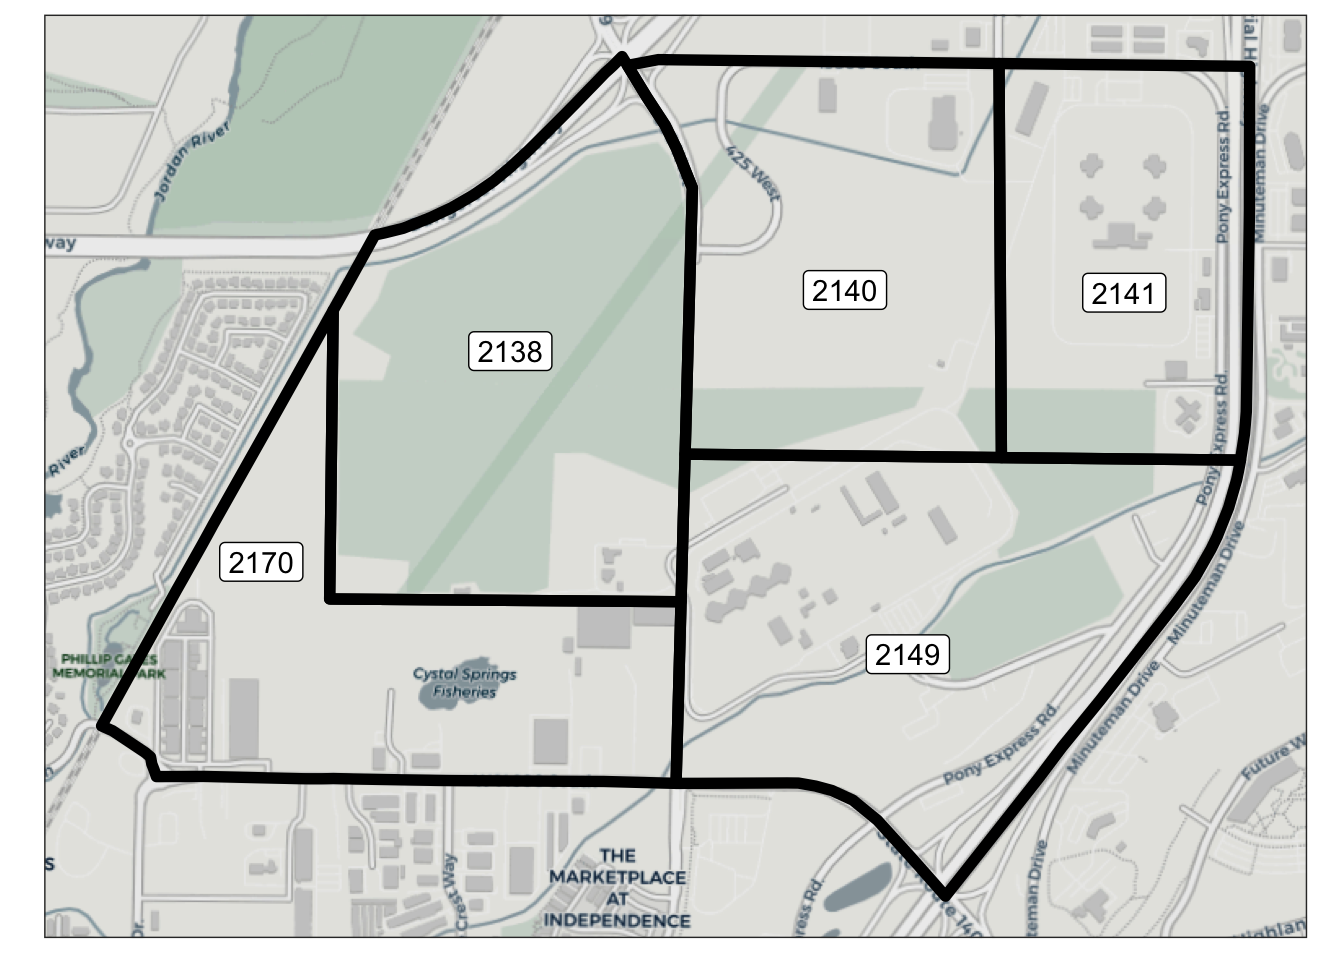
\includegraphics{qmd/1_land_use_files/figure-pdf/fig-the-point-zones-1.png}

}

\caption{\label{fig-the-point-zones}Map of each TAZ in The Point
development.}

\end{figure}%

\begin{table}

\caption{\label{tbl-the-point-data-old}TAZ-level Socioeconomic Data for
The Point (Baseline Scenario)}

\centering{

\centering
\resizebox{\ifdim\width>\linewidth\linewidth\else\width\fi}{!}{
\begin{tabular}[t]{ccccccc}
\toprule
\multicolumn{3}{c}{ } & \multicolumn{4}{c}{Employment} \\
\cmidrule(l{3pt}r{3pt}){4-7}
TAZ & Households & Population & Retail & Industrial & Other & Total\\
\midrule
2138 & 0 & 0 & 0 & 0 & 0 & 0\\
2140 & 0 & 0 & 0 & 0 & 0 & 0\\
2141 & 0 & 0 & 0 & 0 & 277 & 277\\
2149 & 0 & 0 & 0 & 0 & 796 & 796\\
2170 & 0 & 0 & 3 & 359 & 71 & 433\\
\bottomrule
\end{tabular}}

}

\end{table}%

\begin{table}

\caption{\label{tbl-the-point-data-new}TAZ-level Socioeconomic Data for
The Point (Land Use Scenario)}

\centering{

\centering
\resizebox{\ifdim\width>\linewidth\linewidth\else\width\fi}{!}{
\begin{tabular}[t]{ccccccc}
\toprule
\multicolumn{3}{c}{ } & \multicolumn{4}{c}{Employment} \\
\cmidrule(l{3pt}r{3pt}){4-7}
TAZ & Households & Population & Retail & Industrial & Other & Total\\
\midrule
2138 & 7431 & 17811 & 4 & 0 & 76 & 80\\
2140 & 0 & 0 & 610 & 4 & 7390 & 8004\\
2141 & 0 & 0 & 1449 & 0 & 5363 & 6812\\
2149 & 0 & 0 & 962 & 2 & 7372 & 8336\\
2170 & 0 & 0 & 7 & 357 & 106 & 471\\
\bottomrule
\end{tabular}}

}

\end{table}%

\section{Scenario Creation}\label{scenario-creation}

In the WFRC model, this scenario is simple to implement. The model uses
the land use/socioeconomic data directly, so the only adjustment needed
is replacing the data for the specific TAZs with the 2050 forecasted
data. All other TAZs have the same land use data as in the 2019 baseline
scenario.

ActivitySim requires two changes for this scenario. The first is an
update to the TAZ-level land use and socioeconomic data, which is
identical to the process for the WFRC model. The second is an updated
synthetic population. In order to keep consistency between model
scenarios, a new population was created only for the 5 affected TAZs and
joined to the existing synthetic population. There were no individuals
or households in the affected zones in the existing synthetic
population, so no individuals or households needed to be removed before
joining the two populations.

Creating the new synthetic population followed a similar process as in
the baseline scenario (Section~\ref{sec-populationsim}), but used the
new land use data as new TAZ-level controls. Many of the controls for
PopulationSim use tract-level data from the Census, but existing Census
data for The Point site is unrepresentative of the new development, as
currently the site lacks residential and economic activity. Because of
this, the Census tract covering the Gateway area in downtown Salt Lake
City is used to represent the new development patterns at The Point. The
income distribution, etc.~of The Point site will therefore match that of
the Gateway area, though the TAZ-level controls and land
use/socioeconomic data in the area will match the WFRC projections for
2050.

In a more realistic case, a transportation agency would forecast land
use and socioeconomic data that could be used as controls to
PopulationSim, rather than using a separate Census tract to represent
new development. However, our ActivitySim implementation only needs to
be within a rough approximation of the WFRC model for the purposes of
this project, and the method used here results in reasonable accuracy
between the models. Additionally, our ActivitySim implementation is
designed to be independent from the WFRC model where feasible.

\section{Scenario Analysis}\label{scenario-analysis}

There are several kinds of analyses an agency likely would want to do in
assessing the effects of a change in land use. Chief among them would be
an analysis of the new trips resulting from the development. These
analyses could include the number of trips, the distance traveled, and
where the trips are being made.

Both model types allow for very easy analysis of trip numbers and
lengths, as the WFRC model outputs origin-destination trip tables
directly by mode and purpose, and ActivitySim outputs a list of trips
containing information on origin, destination, and mode. Figures
\ref{fig-lu-personmiles-cube} and \ref{fig-lu-personmiles-asim}, for
example, show the new trip-miles produced in the updated zones for the
WFRC model and ActivitySim, respectively. However, there is a crucial
difference between the model types, and that is the treatment of trips
that do not begin or end at the home.

\begin{sidewaysfigure}[p]

\centering{

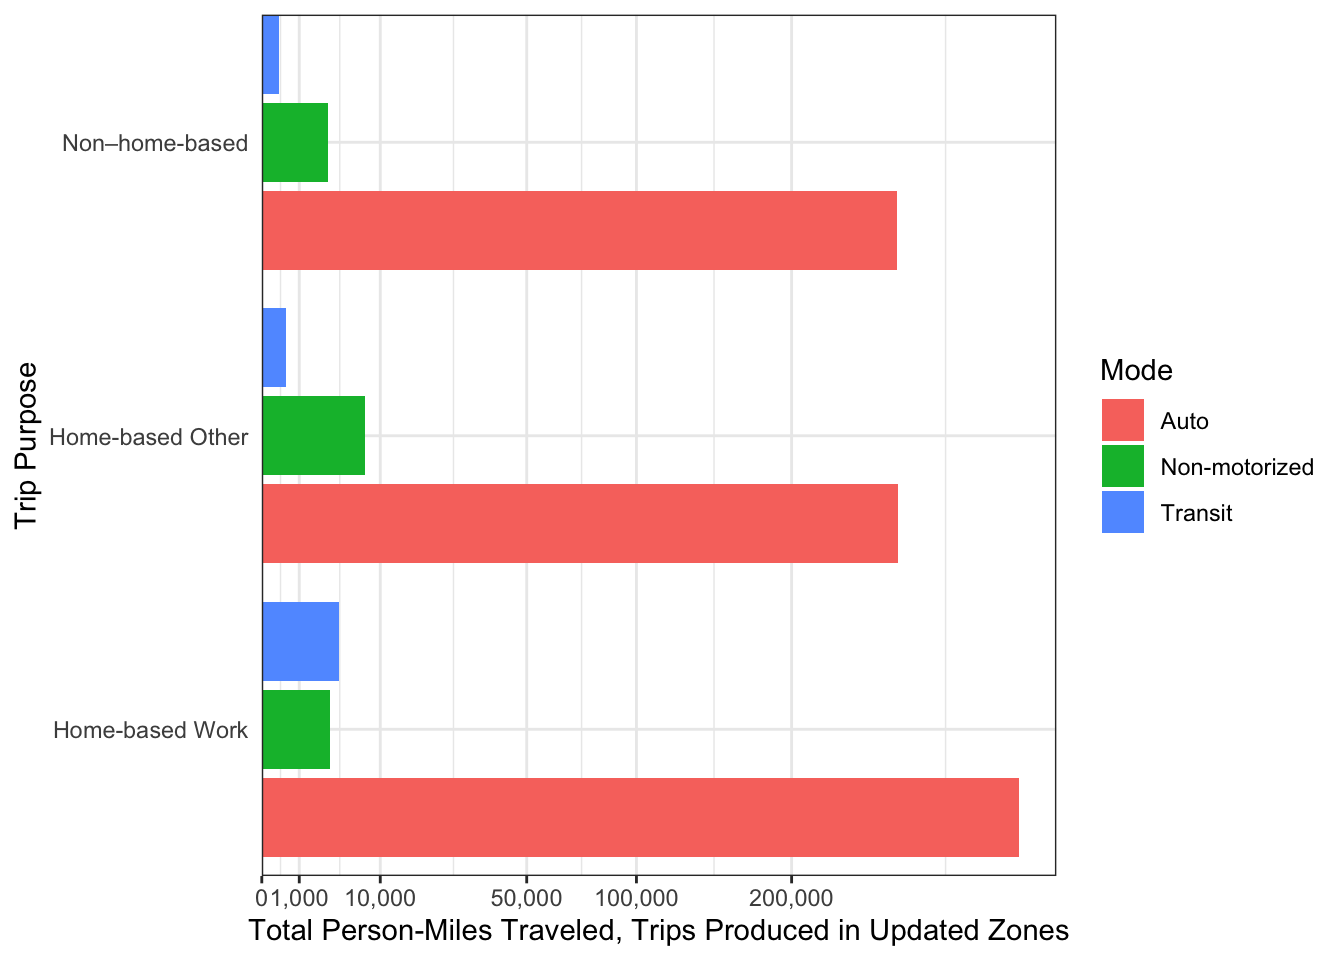
\includegraphics{qmd/1_land_use_files/figure-pdf/fig-lu-personmiles-cube-1.png}

}

\caption{\label{fig-lu-personmiles-cube}Trip-miles produced in the
updated zones in the Land Use scenario (WFRC model).}

\end{sidewaysfigure}%

\begin{sidewaysfigure}[p]

\centering{

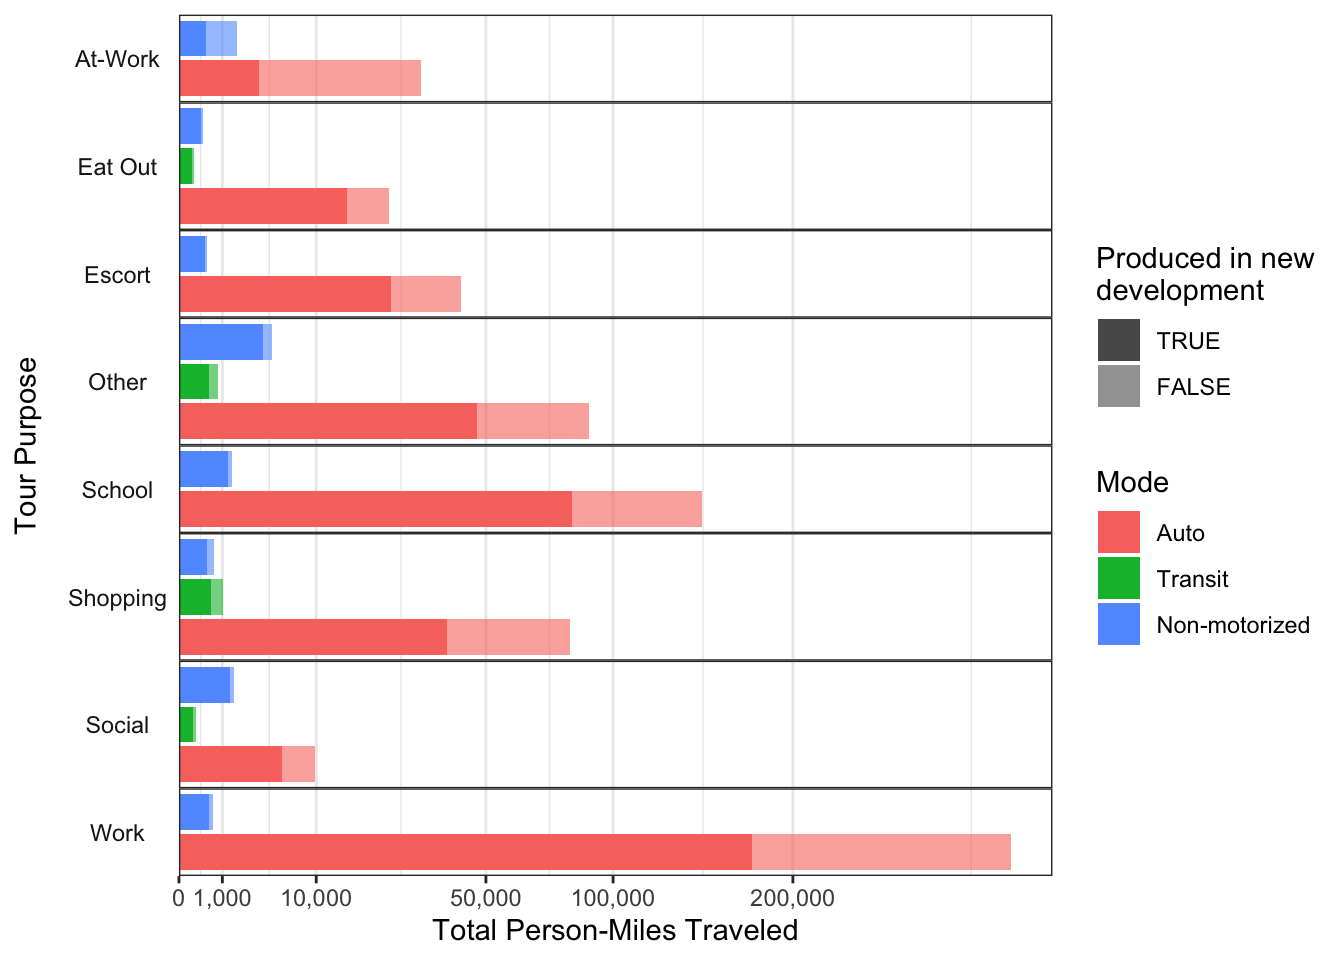
\includegraphics{qmd/1_land_use_files/figure-pdf/fig-lu-personmiles-asim-1.png}

}

\caption[Trip-miles of individuals living in the updates zones
(ActivitySim).]{\label{fig-lu-personmiles-asim}Trip-miles of individuals
living in the updates zones (ActivitySim). Note that many of these trips
do not have an origin or destination in the home zone of the
individual.}

\end{sidewaysfigure}%

In the WFRC model (and in many trip-based models), homes produce trips
with different trip purposes, including Home-based Work, Home-based
Other, and Non--home-based trips. ``Home-based'' trips have an origin or
destination at the home, and are fairly straightforward to model, as the
destination choice step can take for granted that these trips have one
trip end in the zone that produced them. In addition to home-based
trips, though, individuals make many ``non--home-based'' trips, which do
not have an origin or destination at the home (e.g.~traveling from work
to a grocery store). Non--home-based trips can be a significant portion
of total travel, as Figure~\ref{fig-lu-personmiles-cube} shows, but are
not as straightforward to model as home-based trips.

Because Non--home-based trips by definition have neither an origin or
destination at the home (where trips are produced in the trip generation
step), these trips happen exclusively between zones that did not produce
them. It is difficult therefore to know how best to redistribute
Non--home-based trips, as they could in reality have any number of
origins and/or destinations. Though modeling the destination choice for
Non--home-based trips could be done via a similar process to that of
home-based trips, the origins of these trips need to be modeled as well.
There are several methods to redistribute Non--home-based trips in
trip-based models. One approach is to assign Non--home-based trip
origins in a similar manner to trip destinations as part of the trip
distribution step, either with a gravity model or some distance-decay
function. The destinations of these Non--home-based trips can then be
assigned as if they were any other trip. This results in Non--home-based
trips that are more likely to have both an origin and destination
relatively near to the home. The WFRC model takes a different approach.
Here there are two sources of information for Non--home-based trip ends:
a production model and an attraction model. In the trip generation step,
households produce Non--home-based trips similarly to any other trip
purpose. However, the trips produced in this step determine only the
\emph{quantity} of Non--home-based trips, not the trip ends. The
\emph{distribution} of Non--home-based trips is determined by a trip
attraction model, largely based on TAZ employment. This distribution is
then globally scaled to match the total quantity of Non--home-based
trips produced in the trip generation step.

By contrast, an ABM models individuals and their travel explicitly, and
this makes the treatment of Non--home-based trips much more
straightforward. Each trip is tied to a specific individual with a
defined home location, and so no extra ``redistribution'' step is needed
to analyze Non--home-based trips: these are ``built-in'' to each
individual's tour pattern. In fact, as
Figure~\ref{fig-lu-personmiles-asim} shows, Non--home-based trips can
occur as part of any tour type/purpose; there is no separate
``Non--home-based'' purpose in ActivitySim. Note that
Figure~\ref{fig-lu-personmiles-asim} counts person-miles by \emph{tour}
purpose, using the purposes as defined in ActivitySim, rather than
converting the ActivitySim trips to the ``common'' trip purposes as
discussed in Section~\ref{sec-baseline-calibration}.

In addition to looking at total person-miles traveled, it is also useful
to analyze the origins and destinations of the new trips. One common way
to visualize trip origins and destinations is with desire lines, which
show lines for each trip origin/destination pair. The thickness of the
line represents the number of trips between the pair of zones.

Figure~\ref{fig-lu-desire-cube-hb} shows a desire line plot by mode of
all home-based trips produced in the new development zones in the WFRC
model. This figure is in line with what is expected: non-motorized trips
are quite short, transit trips are exclusively to downtown areas, and
many drive alone and carpool trips are made with varying lengths.
Figure~\ref{fig-lu-desire-cube-hb} also shows a similar mode split to
Figure~\ref{fig-lu-personmiles-cube}. Although the former depicts the
\emph{number} of trips and the latter depicts trip \emph{distance},
there is a rough correlation between trip count and miles traveled, so
it is not surprising that the mode split is similar between the figures.

\begin{sidewaysfigure}[p]

\centering{

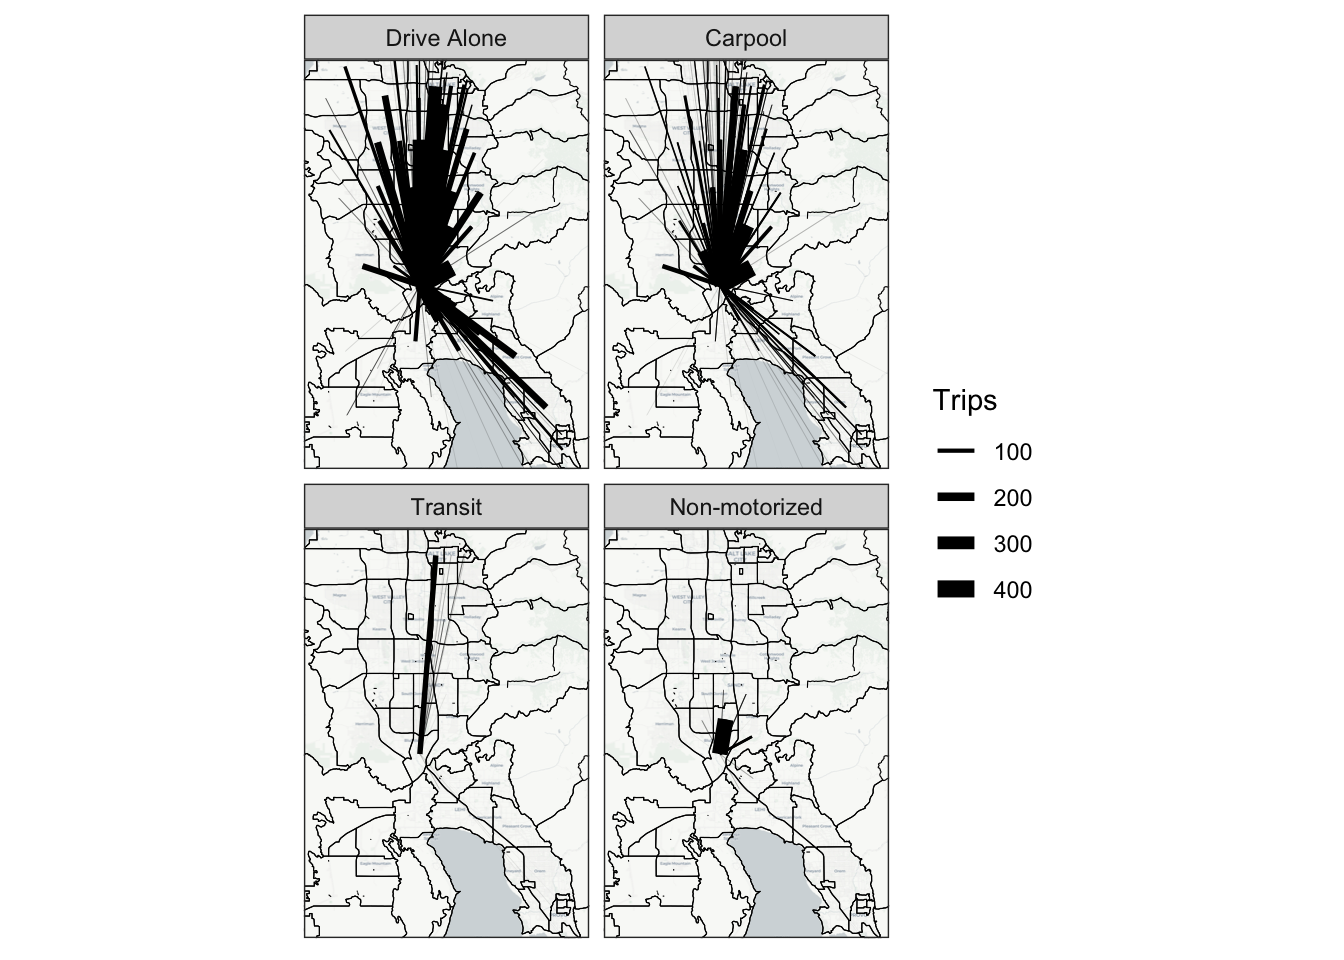
\includegraphics{qmd/1_land_use_files/figure-pdf/fig-lu-desire-cube-hb-1.png}

}

\caption[Desire lines of home-based trips made in the WFRC
model.]{\label{fig-lu-desire-cube-hb}Desire lines of home-based trips
produced in the new development in the WFRC model, by mode.}

\end{sidewaysfigure}%

There is difficulty in analyzing the Non--home-based trips, however.
Typically in a trip-based model, once Non--home-based trips are assigned
trip ends, they have no connection to the homes/zones that produced
them, and are treated as ``belonging'' to either the origin or
destination zone. Because of this, it is not possible to simply filter
trips by origin or destination as can be done with the home-based trips.
Instead, we took the difference between the entire Non--home-based trip
matrices in both this scenario and the baseline scenario.

Figure~\ref{fig-lu-desire-cube-nhb} shows the desire line plot for the
difference in Non--home-based trips between this scenario and the
baseline scenario. Two things are immediately noticeable from this plot.
The first observation is that many pairs of zones saw a decrease in
Non--home-based trips between them compared to the baseline scenario
(i.e.~there were more Non--home-based trips in the baseline scenario
between these zones). Certainly it makes little sense to predict
\emph{fewer} trips as the result of added population and employment.
However, this is in fact not an \emph{overall} decrease in
Non--home-based trips; these trips are simply being assigned trip ends
in different locations due to the nearby change in land use. The second
observation is that the largest increases in Non--home-based trips
include an origin or destination in the new development, i.e.~the home
zones of the new population. Because the change in employment was much
more significant than the change in population (see Tables
\ref{tbl-the-point-data-old} and \ref{tbl-the-point-data-new}), many
more Non--home-based trip ends were attracted to the development zones
compared to the relatively little global increase in Non--home-based
trips due to the increase in population. Both effects (the global
increase in and the changed distribution of Non--home-based trips) are
present in the model, but the two effects are impossible to separate.

\begin{sidewaysfigure}[p]

\centering{

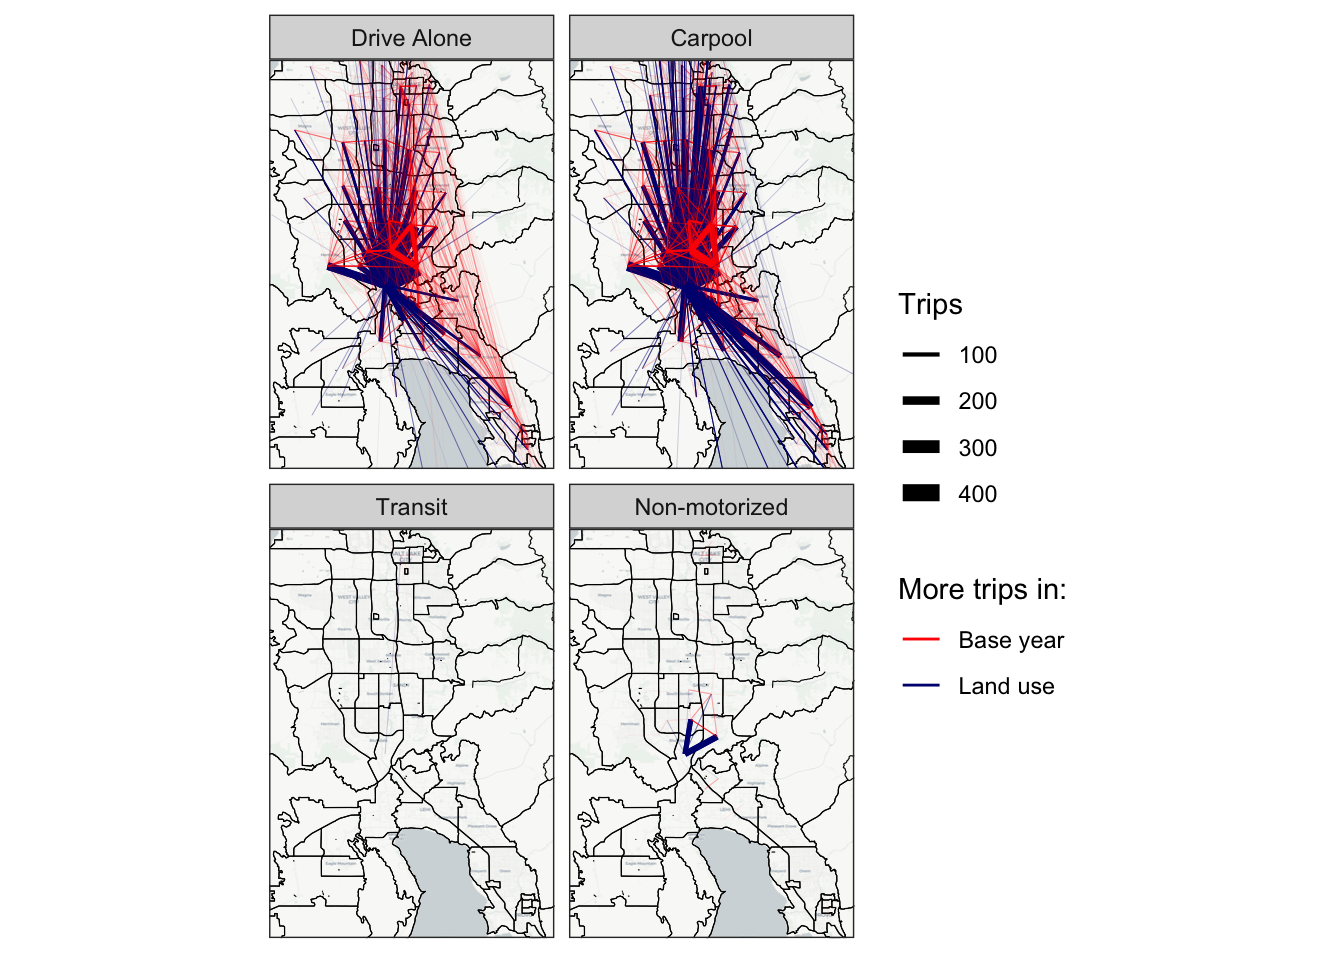
\includegraphics{qmd/1_land_use_files/figure-pdf/fig-lu-desire-cube-nhb-1.png}

}

\caption[Desire lines of Non--home-based trips made in the WFRC
model.]{\label{fig-lu-desire-cube-nhb}Desire lines of Non--home-based
trips made in the WFRC model, by mode. Note that the trip counts are
obtained by differencing the Non--home-based trip matrix with the base
year.}

\end{sidewaysfigure}%

As mentioned, an ABM allows for tracking of individuals explicitly, and
so analyzing Non--home-based trips is much more straightforward.
Figure~\ref{fig-lu-desire-asim} shows desire lines of all trips made by
individuals living in the new development zones for ActivitySim.
Non--home-based trips are colored differently from home-based trips.

It is easy to connect Non--home-based trips to their place of
production, as each trip is linked to a specific individual who has a
defined home location. It is also easy to see how trips are related to
each other, as each individual has a specific sequence of trips. The
individual nature of an ABM avoids entirely the problems trip-based
models have with Non--home-based trips. In a complicated land use
forecast, each development's full contribution to network congestion can
be analyzed individually.

\begin{sidewaysfigure}[p]

\centering{

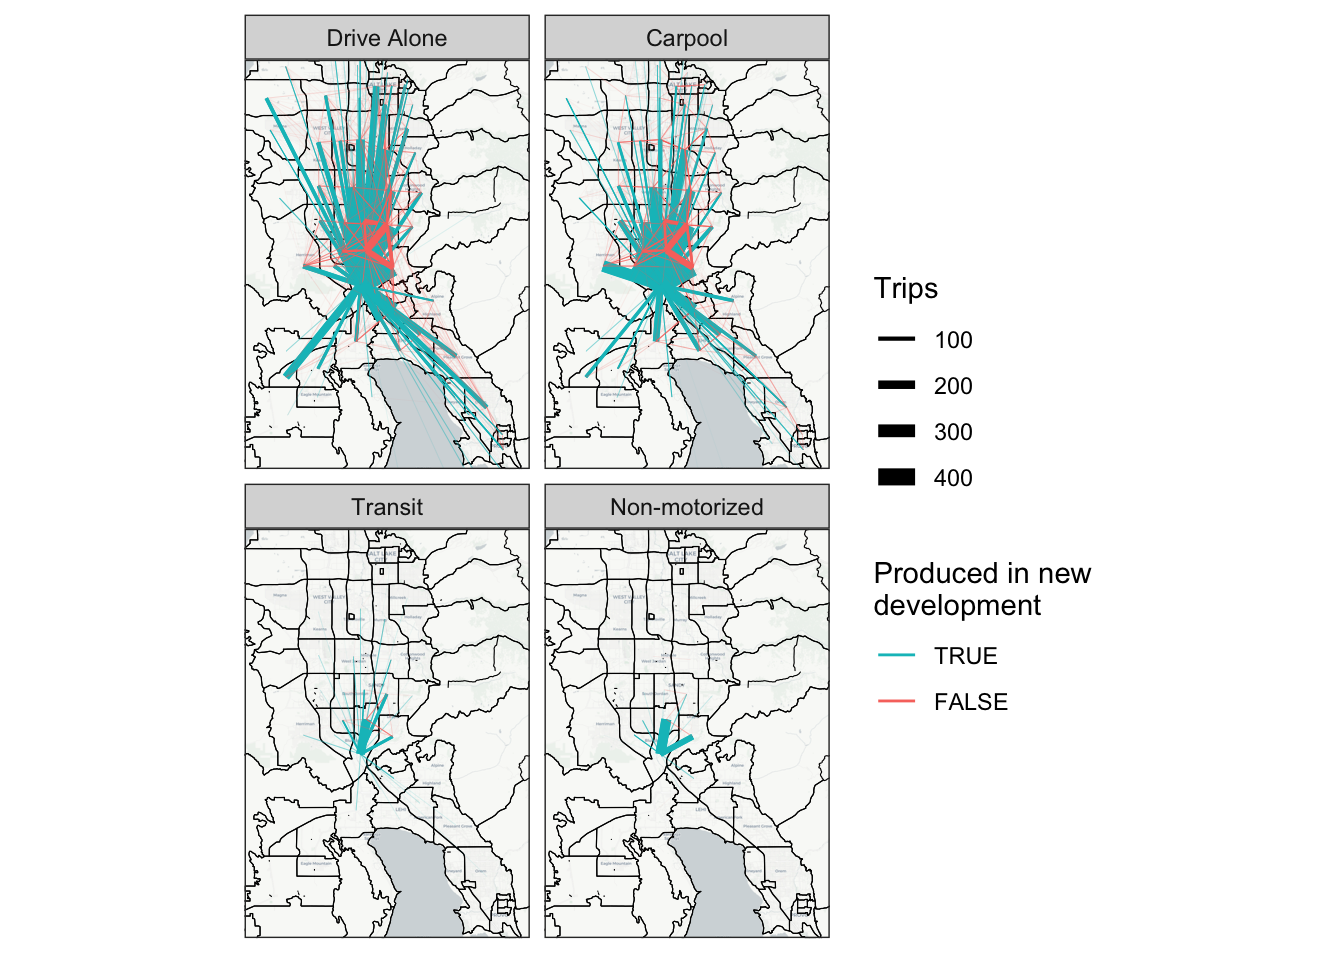
\includegraphics{qmd/1_land_use_files/figure-pdf/fig-lu-desire-asim-1.png}

}

\caption{\label{fig-lu-desire-asim}Desire lines of trips made in
ActivitySim by mode.}

\end{sidewaysfigure}%

\bookmarksetup{startatroot}

\chapter{Scenario 2: Improved Transit Service}\label{sec-transit}

Our second scenario models changes in travel behavior as a result of
changes to transportation infrastructure. This model scenario, termed
the ``Transit'' scenario, is based on a planned improvement to the
FrontRunner commuter rail line. The FrontRunner runs along the Wasatch
Front between Provo and Ogden, Utah, with several stops in between.
Currently, there is only one set of tracks for much of the line, and it
is only possible for trains to pass each other near stations. Because of
this, headways are quite large, with trains running every half-hour in
peak periods and hourly in off-peak periods.

A potential improvement to the FrontRunner would ``double track'' the
entire route, allowing trains to pass each other at any point. The main
benefit of this improvement is a substantial decrease in headways,
bringing them to 15 and 30 minutes for peak and off-peak service,
respectively. Two additional improvements are partial electrification of
the FrontRunner, allowing for faster travel speeds, and extending the
track farther south with additional stops.

The Transit scenario models these improvements to the FrontRunner. The
scenario adjusts the headways to 15/30 minutes for peak/off-peak
service, increases travel speeds, and adds additional stops in
Vineyard\footnote{In 2019, the model year for the baseline scenario, the
  Vineyard station was not yet open, though the station has been
  operational since late 2022.}, Springville, Spanish Fork, and Payson.
Figure~\ref{fig-frontrunner-map} shows the FrontRunner network along
with the modeled changes. In reality there would be additional transit
improvements, such as a revised bus service network serving the
Springville station, but for the sake of simplicity these additional
improvements are not included in this model scenario. Only the changes
to the FrontRunner service are modeled here.

\begin{figure}[p]

\centering{

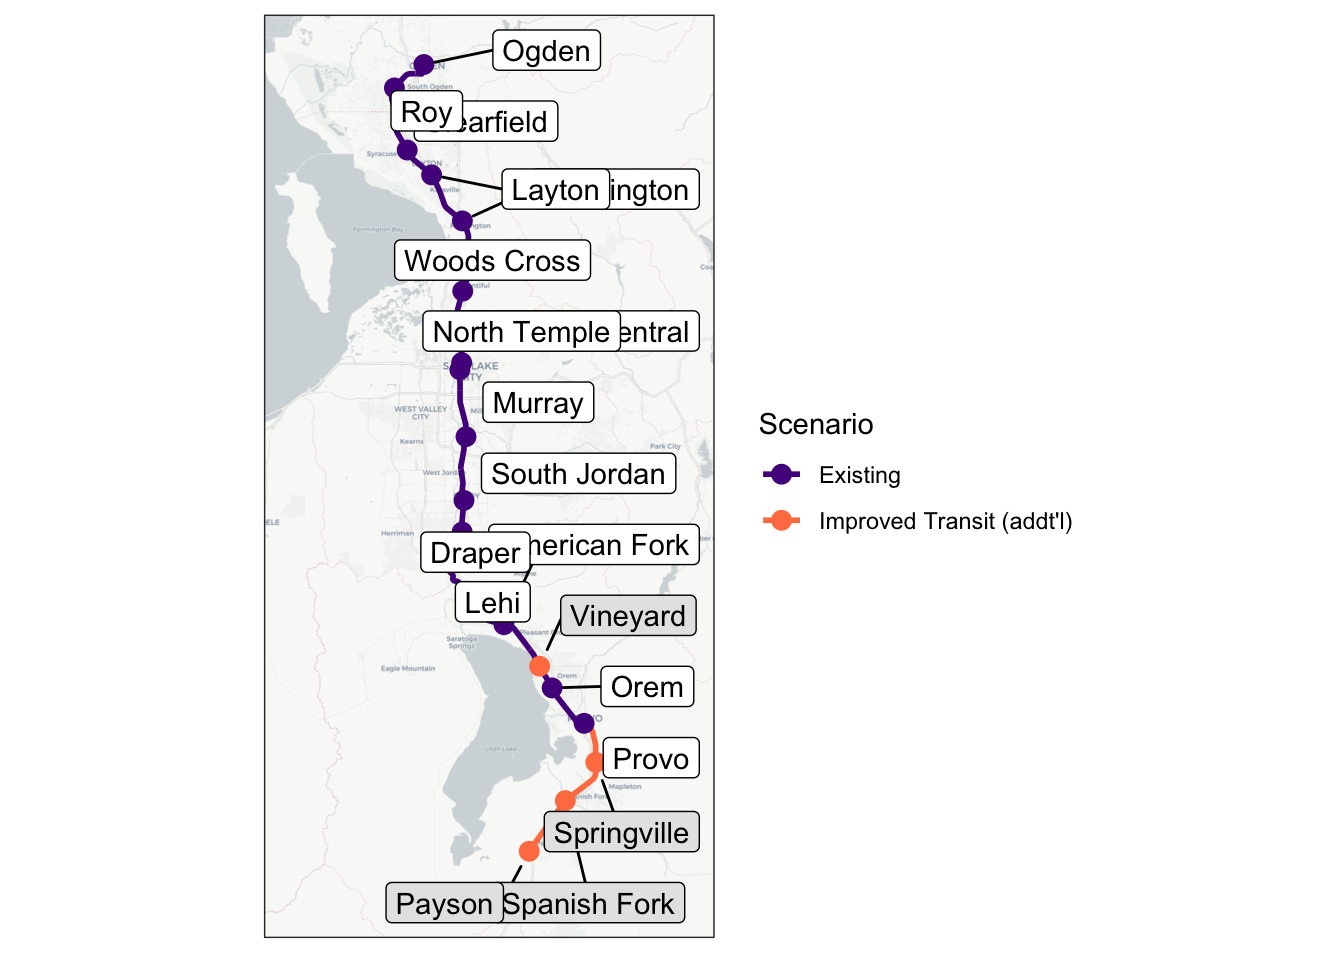
\includegraphics{qmd/2_transit_files/figure-pdf/fig-frontrunner-map-1.png}

}

\caption{\label{fig-frontrunner-map}Map of the FrontRunner commuter rail
line.}

\end{figure}%

\section{Scenario Creation}\label{scenario-creation-1}

In the WFRC model, this scenario is relatively easy to implement. The
headways are stored directly in the input data and are easily modified,
and a year-2050 network with increased speeds and additional stations is
already built into the model for future-year analysis. The only
additional change needed was to turn on the ``park and ride'' flag in
the highway network at the node of each new station, which allows
transfers between auto and transit modes at these nodes.

To implement this scenario in ActivitySim, only updated travel skims are
needed. As in the baseline scenario, ActivitySim directly uses the
transit skims that are output from the WFRC model's network assignment
in this model scenario. Because the mode share of transit is relatively
low, it is not expected that the highway travel times will be affected
very much by this change. The highway skims used for ActivitySim are
therefore taken from the WFRC model baseline scenario and not updated
for this scenario. No other changes to ActivitySim are necessary to
model this scenario.

\section{Scenario Analysis}\label{scenario-analysis-1}

One of the most straightforward analyses to perform is a comparison of
the mode split between this and the baseline scenario.
Table~\ref{tbl-tr-mode-split} shows the number of trips by purpose and
mode for each model, and compares these results between this scenario
and the baseline scenario (\emph{n.b.} ``local transit'' includes both
light rail and bus travel). Unsurprisingly, both models predict a
significant increase in commuter rail trips. The models differ, however,
in which modes the new commuter rail trips come from.

\begin{sidewaystable}

\caption{\label{tbl-tr-mode-split}Change in Mode Split with Improved
Transit}

\centering{

\centering
\resizebox{\ifdim\width>\linewidth\linewidth\else\width\fi}{!}{
\begin{tabular}[t]{cccccccc}
\toprule
\multicolumn{2}{c}{ } & \multicolumn{3}{c}{WFRC Model} & \multicolumn{3}{c}{ActivitySim} \\
\cmidrule(l{3pt}r{3pt}){3-5} \cmidrule(l{3pt}r{3pt}){6-8}
Purpose & Mode & Baseline Trips & Transit¹ Trips & Change & Baseline Trips & Transit¹ Trips & Change\\
\midrule
 & Drive Alone & 1328609 & 1326191 & -0.2\% & 1012180 & 1010565 & -0.2\%\\

 & Carpool & 257783 & 256654 & -0.4\% & 258459 & 256550 & -0.7\%\\

 & Local Transit & 37935 & 36494 & -3.8\% & 232222 & 233426 & 0.5\%\\

 & Commuter Rail & 10821 & 15891 & 46.9\% & 19846 & 22265 & 12.2\%\\

 & Ridehail & — & — & — & 1108 & 1099 & -0.8\%\\

\multirow{-6}{*}{\centering\arraybackslash Home-based Work} & Non-motorized & 76506 & 76396 & -0.1\% & 145957 & 145845 & -0.1\%\\
\cmidrule{1-8}
 & Drive Alone & 1394415 & 1394095 & 0.0\% & 700133 & 698809 & -0.2\%\\

 & Carpool & 2702277 & 2701039 & 0.0\% & 2148429 & 2145135 & -0.2\%\\

 & Local Transit & 33168 & 32583 & -1.8\% & 195062 & 194649 & -0.2\%\\

 & Commuter Rail & 4180 & 6332 & 51.5\% & 81094 & 87337 & 7.7\%\\

 & Ridehail & — & — & — & 113624 & 113538 & -0.1\%\\

\multirow{-6}{*}{\centering\arraybackslash Home-based Other} & Non-motorized & 510143 & 510103 & 0.0\% & 613134 & 611996 & -0.2\%\\
\cmidrule{1-8}
 & Drive Alone & 951561 & 951407 & 0.0\% & 716143 & 714854 & -0.2\%\\

 & Carpool & 1273279 & 1272977 & 0.0\% & 938056 & 936408 & -0.2\%\\

 & Local Transit & 12213 & 12068 & -1.2\% & 107526 & 108395 & 0.8\%\\

 & Commuter Rail & 1243 & 1806 & 45.3\% & 12317 & 13344 & 8.3\%\\

 & Ridehail & — & — & — & 40092 & 40061 & -0.1\%\\

\multirow{-6}{*}{\centering\arraybackslash Non–home-based} & Non-motorized & 146404 & 146409 & 0.0\% & 156819 & 156587 & -0.1\%\\
\bottomrule
\multicolumn{8}{l}{\rule{0pt}{1em}\textsuperscript{1} "Transit" here refers to the Transit scenario, not the mode of travel}\\
\end{tabular}}

}

\end{sidewaystable}%

For Home-based Other and Non--home-based trips, the WFRC model shows
virtually no change in the number of auto and non-motorized trips, while
there is a significant decrease in the number of local transit trips.
Home-based Work trips do see a decrease in auto trips with the improved
transit, but there are still significantly fewer local transit trips
compared to the baseline scenario. This indicates that the new commuter
rail trips are mostly coming from those who would have taken local
transit in the baseline scenario.

ActivitySim, on the other hand, actually shows an \emph{increase} in
local transit trips for Home-based Work and Non--home-based trips. For
Home-based Other trips, there is a decrease in local transit, but by
percentage it is not nearly as significant as the decrease in the WFRC
model.\footnote{The absolute difference in \emph{number} of Home-based
  Other local transit trips between the scenarios is comparable between
  the two models, but since ActivitySim is predicting significantly more
  transit trips in the baseline scenario compared to the WFRC model, the
  percent change is much smaller in ActivitySim.} This shows that most
new commuter rail trips in ActivitySim are coming from auto (drive alone
and carpool) modes, rather than other transit modes.

The discrepancy may be partially explained by the difference in the way
trips are modeled. In the WFRC model, trips are modeled in aggregate,
with no interaction between separate trips. Regardless of trip purpose,
trips are treated essentially the same, though potentially with
different coefficients in mode choice equations. Even Non--home-based
trips are treated like any other trip during mode choice. Additionally,
there is a nesting structure to the mode choice step in the WFRC model.
The transit ``nest'' contains all transit modes, and so when the
commuter rail service is improved the utility of commuter rail compared
to other transit modes increases more than the utility of commuter rail
compared to non-transit modes. Many of the new commuter rail trips
therefore come from those who would have taken transit otherwise.

ActivitySim, however, \emph{does} model interactions between trips. An
individual who makes a commuter rail trip will (usually) not be able to
drive for subsequent trips until they have returned home. Because of
this, individuals taking commuter rail are more likely to then take
other forms of transit on the same tour. There is a similar nesting
structure in the mode choice model of ActivitySim as in the WFRC model,
but this effect is less pronounced in part due the aforementioned
structuring of trips into tours.

One particularly interesting analysis that can be done with an ABM is to
see who changed modes with the improved transit. Because trips are
modeled individually rather than in aggregate, it is possible to
identify trips that switch modes between the scenarios.
Figure~\ref{fig-tr-mode-switching} shows the distribution of these
``switched'' trips. These are trips that are ``the same'' between
scenarios and differ only by mode. For the purposes of this analysis,
trips are considered ``the same'' between scenarios if they are made by
the same person and have the same origin and destination zones, time of
day\footnote{ActivitySim models time of day as the ``departure hour''
  for each trip. If two trips share the same departure hour, they are
  considered here to have happened at the same time.}, and tour and trip
purpose. Most of these trips also share the same mode, which is to be
expected, but many do not. Figure~\ref{fig-tr-mode-switching} is
filtered to show only trips that do not share the same mode between
scenarios.

\begin{sidewaysfigure}[p]

\centering{

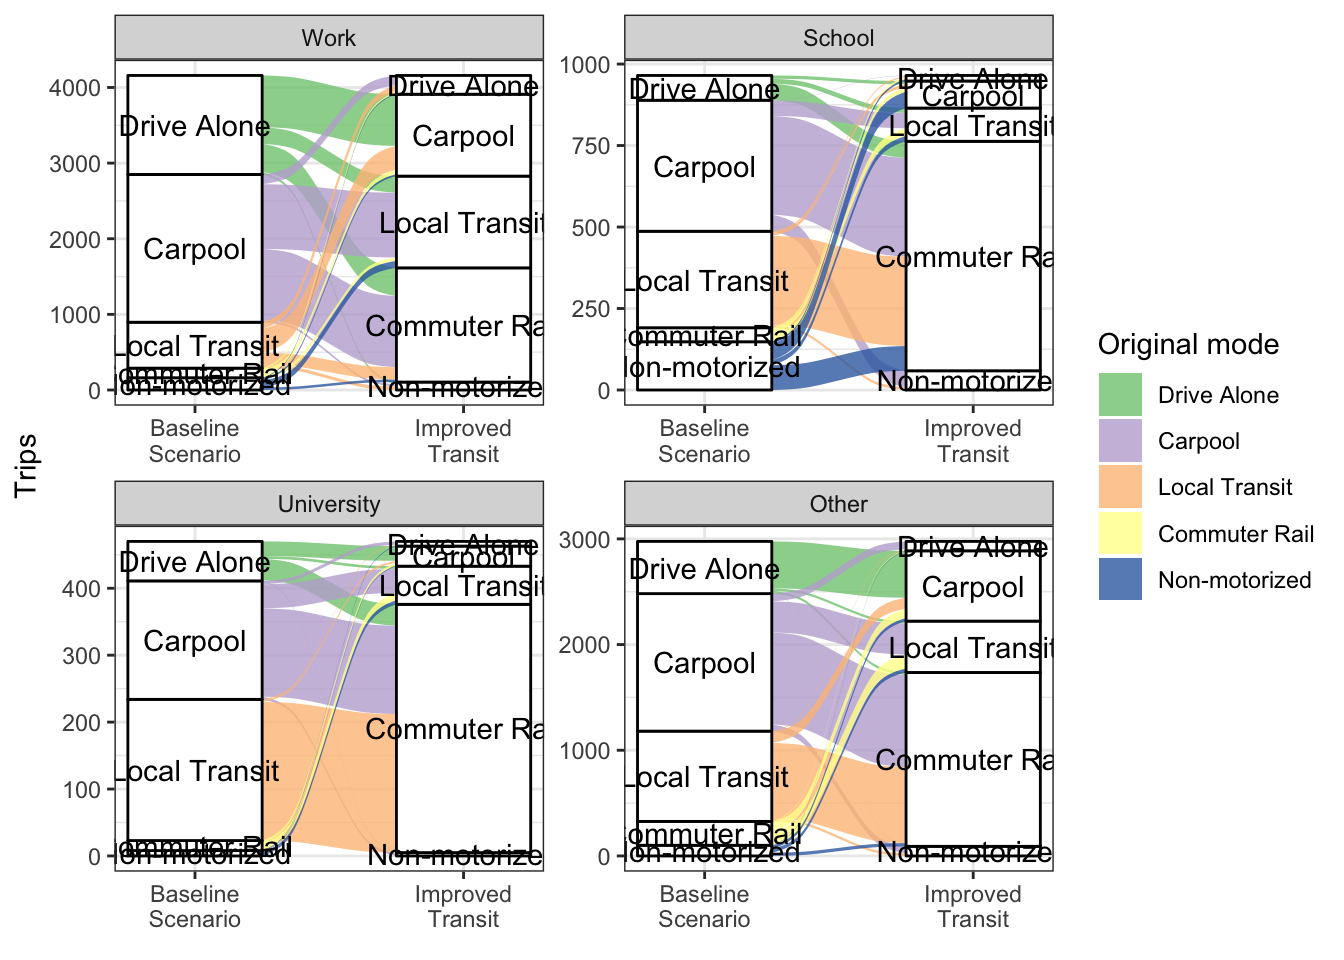
\includegraphics{qmd/2_transit_files/figure-pdf/fig-tr-mode-switching-1.png}

}

\caption[Trip modes of individuals who switched modes with improved
commuter rail service.]{\label{fig-tr-mode-switching}Trip modes of
individuals who switched modes with improved commuter rail service, by
tour purpose.}

\end{sidewaysfigure}%

There is some amount of randomness in the way ActivitySim determines
trip modes, though. This randomness is seen partly in trips that switch
away from commuter rail despite the improved commuter rail service, as
well as some trips that switch to modes other than commuter rail,
especially to drive alone. Although, part of the switch from carpool to
drive alone can be explained as previously-carpool trips where all but
one vehicle occupant switched to another mode, leaving one person in the
vehicle for the trip. Overall, though, the randomness is not a
significant percentage of the overall mode switching seen in
Figure~\ref{fig-tr-mode-switching}.

Mode choice is not the only step of ActivitySim affected by the improved
transit service, however. In fact, there are many trips that do not have
a match between scenarios, where origin, destination, time of day and/or
purpose differ. The number of trips an individual makes may also differ
between scenarios, as each person's DAP is partially dependent on
accessibility measures (see Figure~\ref{fig-asim-flowchart}). Notably,
Figure~\ref{fig-tr-mode-switching} also does not include any of these
trips; the figure only shows trips which do have a match between
scenarios.

ABMs also allow for even more granular analysis than shown in
Figure~\ref{fig-tr-mode-switching}. For example,
Figure~\ref{fig-tr-atwork-switching} shows the trip modes of at-work
subtours made by individuals who switched their work tour mode away from
drive alone. The figure shows the at-work subtour trip modes for
\emph{all} these individuals, not just those who also switched their
at-work subtour trip modes. These results are essentially as expected.
All trips that were drive alone in the baseline scenario switched to
carpool, and there was virtually no mode switching otherwise, except a
few trips that switched from carpool to non-motorized. This switching
can again be largely explained by the randomness in ActivitySim's mode
choice models, and again is relatively insignificant.

\begin{figure}

\centering{

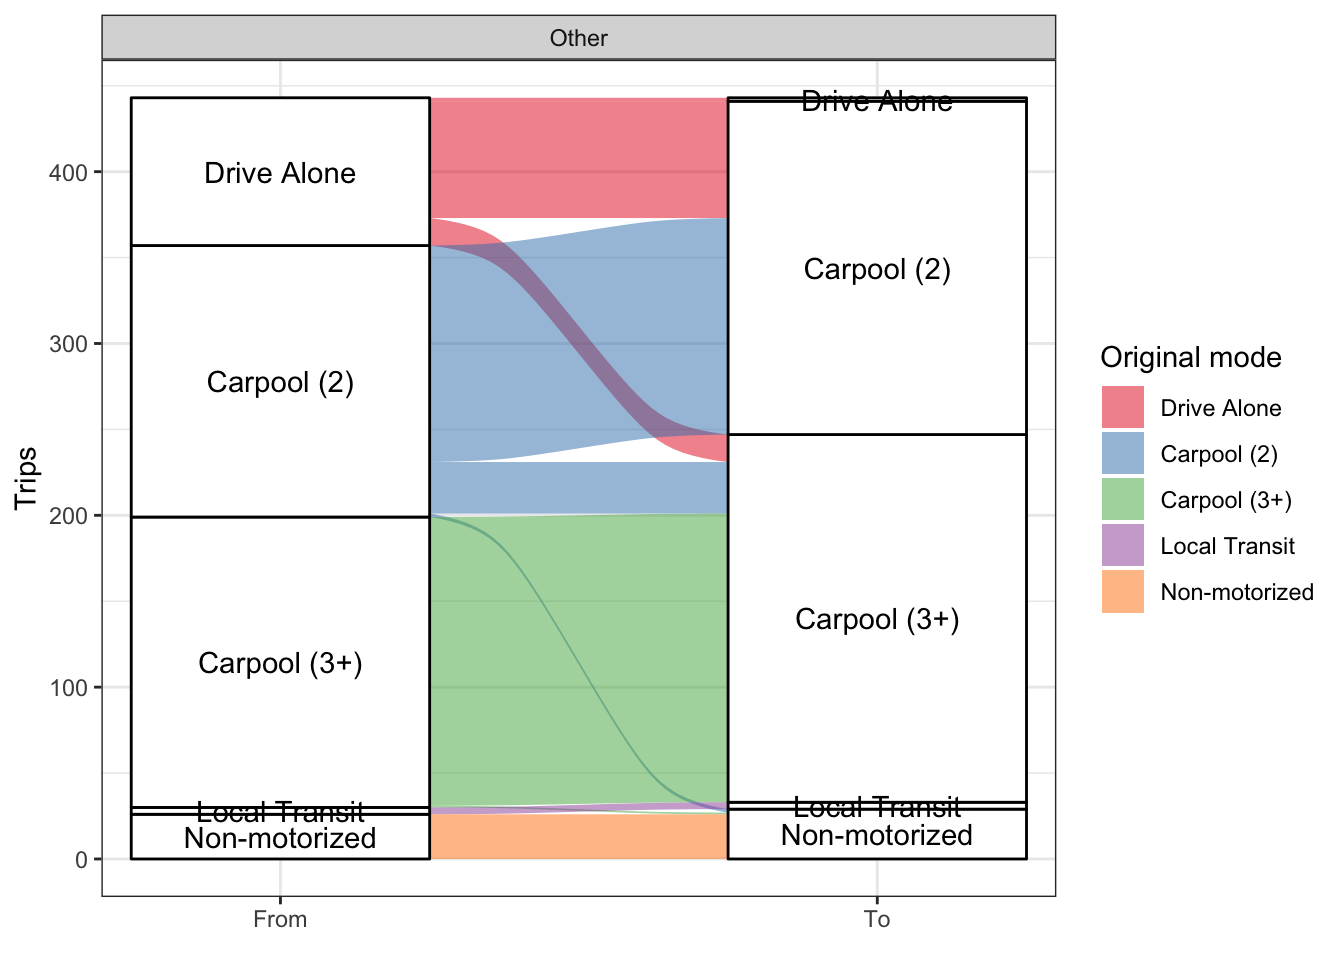
\includegraphics{qmd/2_transit_files/figure-pdf/fig-tr-atwork-switching-1.png}

}

\caption{\label{fig-tr-atwork-switching}At-work subtour trip modes of
individuals who switched their work mode away from ``Drive Alone''.}

\end{figure}%

Both model types additionally allow for analyzing the types of people
who use transit. The WFRC model, however, is limited to analyses using
aggregate, TAZ-level data. Table~\ref{tbl-tr-cube-se} shows, for
example, the median number of households, people, and jobs weighted by
the number of transit trip productions in each TAZ for the WFRC model.
Additionally, Table~\ref{tbl-tr-cube-se} shows a median income
associated with transit trips, but note that this is not a median income
of transit \emph{riders}, but a median of \emph{TAZ median income},
weighted by trip productions. It is difficult to know the actual income
distribution of transit riders since individuals are not modeled
explicitly.

\begin{table}

\caption{\label{tbl-tr-cube-se}Example Socioeconomic Analysis of Transit
Trips (WFRC Model)}

\centering{

\centering
\resizebox{\ifdim\width>\linewidth\linewidth\else\width\fi}{!}{
\begin{tabular}[t]{ccccccc}
\toprule
\multicolumn{3}{c}{ } & \multicolumn{4}{c}{TAZ-level Median (weighted by trips)} \\
\cmidrule(l{3pt}r{3pt}){4-7}
Purpose & Mode & Trips & Households & Population & Employment & Income\\
\midrule
 & Local Transit & 36494 & 478 & 1211 & 400 & \$54,208\\

\multirow{-2}{*}{\centering\arraybackslash Home-based Work} & Commuter Rail & 15891 & 435 & 1368 & 279 & \$76,529\\
\cmidrule{1-7}
 & Local Transit & 32583 & 460 & 1147 & 454 & \$49,682\\

\multirow{-2}{*}{\centering\arraybackslash Home-based Other} & Commuter Rail & 6332 & 423 & 1306 & 317 & \$68,369\\
\cmidrule{1-7}
 & Local Transit & 12068 & 97 & 182 & 1362 & \$50,921\\

\multirow{-2}{*}{\centering\arraybackslash Non–home-based} & Commuter Rail & 1806 & 138 & 453 & 1487 & \$58,576\\
\bottomrule
\end{tabular}}

}

\end{table}%

Because an ABM \emph{does} model individuals explicitly, information
about each individual is accessible at every stage of the model,
including in post-hoc analysis. We can therefore determine the actual
distribution of e.g.~age and income for transit riders.
Table~\ref{tbl-tr-asim-se} shows a similar summary as
Table~\ref{tbl-tr-cube-se}, but for ActivitySim.
Table~\ref{tbl-tr-asim-se} presents median values for the individuals
who made transit trips, not simply TAZ averages. Notably, Tables
\ref{tbl-tr-cube-se} and \ref{tbl-tr-asim-se} show that ActivitySim is
predicting a higher median income of transit riders than the WFRC model.
Our synthetic population does over-predict high-income households along
the length of the FrontRunner (see Figure~\ref{fig-income-group-map}),
and this may partially be the cause of the discrepancy.

\begin{table}

\caption{\label{tbl-tr-asim-se}Example Socioeconomic Analysis of Transit
Trips (ActivitySim)}

\centering{

\centering
\resizebox{\ifdim\width>\linewidth\linewidth\else\width\fi}{!}{
\begin{tabular}[t]{cccccc}
\toprule
\multicolumn{3}{c}{ } & \multicolumn{3}{c}{Individual-level Median} \\
\cmidrule(l{3pt}r{3pt}){4-6}
Purpose & Mode & Trips & Income & Age & Distance to work (mi)\\
\midrule
 & Local Transit & 233426 & \$78,735 & 37 & 7.4\\

\multirow{-2}{*}{\centering\arraybackslash Home-based Work} & Commuter Rail & 22265 & \$85,314 & 33 & 24.3\\
\cmidrule{1-6}
 & Local Transit & 194649 & \$58,408 & 28 & 4.9\\

\multirow{-2}{*}{\centering\arraybackslash Home-based Other} & Commuter Rail & 87337 & \$68,603 & 23 & 3.8\\
\cmidrule{1-6}
 & Local Transit & 108395 & \$63,718 & 33 & 6.2\\

\multirow{-2}{*}{\centering\arraybackslash Non–home-based} & Commuter Rail & 13344 & \$58,408 & 25 & 3.9\\
\bottomrule
\end{tabular}}

}

\end{table}%

Additionally, Figure~\ref{fig-tr-se-income-dist} shows the income
distribution of transit riders for the WFRC model and ActivitySim.
Again, the WFRC model is not modeling individuals, so for the WFRC model
Figure~\ref{fig-tr-se-income-dist} shows the distribution of median TAZ
income weighted by number of trip productions. For ActivitySim, however,
the true income distribution of individual transit riders is shown.

ActivitySim shows a rather wide income distribution of transit riders,
while the distribution of the WFRC model is much denser around
\$50,000--\$75,000. This makes sense given that the WFRC model shows a
distribution of \emph{median} incomes, while ActivitySim shows the
distribution of \emph{individual} incomes. It is clear that ActivitySim
considers transit to be more attractive for a wider range of incomes
than the overall income distribution, though notably low- to
medium-income individuals are somewhat more likely to take transit. In
the WFRC model, however, the income distribution of individuals taking
transit is unknown.

\begin{figure}

\centering{

\includegraphics{qmd/2_transit_files/figure-pdf/fig-tr-se-income-dist-1.png}

}

\caption[Income distribution of transit riders in both
models.]{\label{fig-tr-se-income-dist}Income distribution of transit
riders in both models. The distribution of TAZ median income weighted by
transit trips is used for the WFRC model, while for ActivitySim the
actual income distribution of transit riders is used.}

\end{figure}%

\bookmarksetup{startatroot}

\chapter{Scenario 3: Increase in Remote Work}\label{sec-wfh}

Our final model scenario, termed the ``Remote Work'' scenario, addresses
changes in travel behavior as a result of social and/or economic
factors. Specifically, we represent an increase in remote work rates
since the COVID-19 pandemic. With the onset of the COVID-19 pandemic,
there were unprecedented numbers of people working remotely (Bick et al.
2021). Though remote work is currently not as common as during the
pandemic, remote work rates are increasing each year and are predicted
to continue to rise (Ozimek 2020).

As noted in Section~\ref{sec-baseline-calibration}, both models make a
distinction between ``working from home'' (no work location other than
home) and ``telecommuting'' (working remotely some but not all days).
The WFRC model contains a lookup table of both work-from-home (called
``home-based jobs'' in the WFRC model) and telecommute percentages by
job type and year, and predicts an increase in both remote work rates
over time. Figure~\ref{fig-wfrc-remote-work-rate-plot} shows the remote
work rates predicted in the WFRC model by year.

\begin{figure}

\centering{

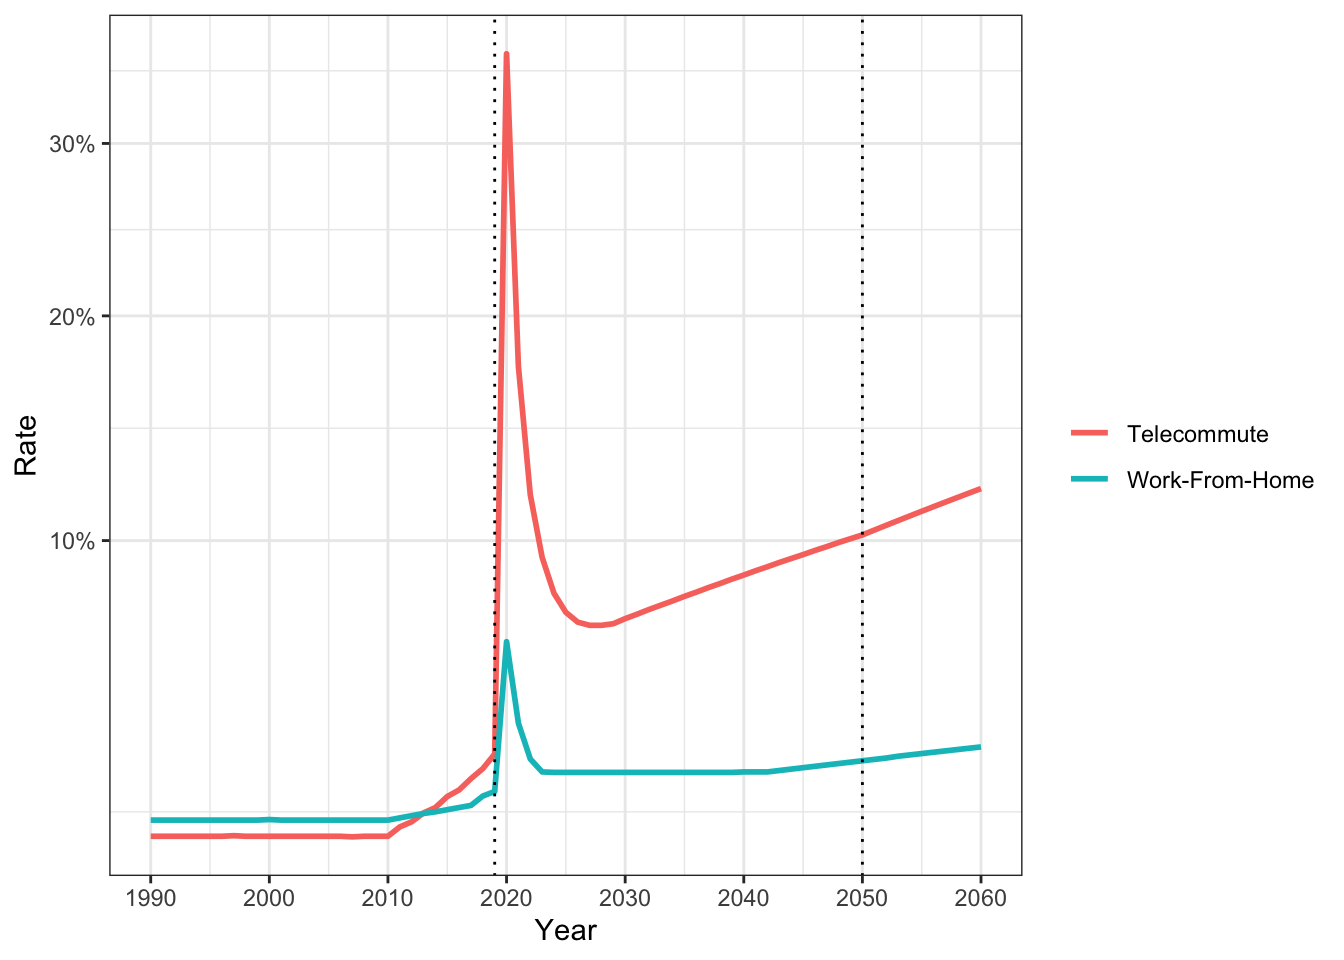
\includegraphics{qmd/3_wfh_files/figure-pdf/fig-wfrc-remote-work-rate-plot-1.png}

}

\caption{\label{fig-wfrc-remote-work-rate-plot}Remote work rates as
given in the WFRC model.}

\end{figure}%

This scenario is a ``what-if'' analysis that models a significant
increase in remote work rates. We use the remote work rates from 2050 as
predicted by the WFRC model, but make no other changes from the baseline
scenario. In other words, this scenario models the 2050 predicted remote
work rates with the 2019 land use and infrastructure.

There has been much research, especially in recent years, on the
implications of remote work. While many agencies have adjusted their
models to account for remote work, and most models follow similar
principles, it is not obvious what the best method is. Bramberga (2023)
even suggests that considerations for remote work should be made on a
case-by-case basis because there is no single best approach. The
following section discusses some of these considerations.

\section{Considerations for Modelling Remote
Work}\label{sec-remote-work-considerations}

Increasing remote work rates may affect several aspects of travel
behavior. The most obvious effect is that people will on average make
fewer work trips, and this effect will vary by job type (Yasenov 2020).
Most travel demand models include a decrease in work trips based on
remote work rates and job type (Bramberga 2023; Moeckel 2017; Sener and
Bhat 2011).

While work trips decrease with an increase in remote work, Kim (2017)
discusses a ``rebound effect'', where individuals make more
discretionary trips on days they do not commute to work. Moreno and
Moeckel (2017) similarly discuss the idea of a ``travel time budget'',
where a decrease in trips of one purpose will increase the time people
allocate for trips of another purpose and vice versa.

This rebound effect is not straightforward, however. Elldér (2020), for
example, finds that distinguishing between people that work from home
all day and those who work form home only part of the day might make a
difference. Compared to those who commute to work, those who worked from
home the entire day had fewer trips and miles traveled, but those who
worked from home only part of the day had more trips and miles traveled.

Additionally, the types of trips people make can differ depending on
remote work status. While the rebound effect proposes that the
\emph{number} of trips may increase on remote work days (see e.g. He and
Hu 2015), Mokhtarian and Varma (1998) find a decrease in vehicle
\emph{miles} traveled for both work and discretionary trips on remote
work days. This implies that longer trips are being replaced by shorter
trips on days people do not travel to work. Moeckel (2017) additionally
finds that those who travel to their job site less frequently are more
likely to live further away from their job site, and so their longer but
infrequent commute is dropped on remote work days, perhaps in favor of
shorter, discretionary trips.

In our case, we are using the existing frameworks for modeling remote
work in both ActivitySim and the WFRC model, as discussed in
Section~\ref{sec-baseline-calibration}.

\section{Scenario Creation}\label{scenario-creation-2}

Two changes are needed in the WFRC model for this scenario. The first is
to replace the 2019 estimates for work-from-home and telecommuting with
the 2050 estimates. Table~\ref{tbl-wfrc-remote-work-years} shows both
the original and updated estimates. The second change is to the
TAZ-level socioeconomic data. The WFRC model estimates a number of
home-based jobs in each TAZ, and the original 2019 home-based job
estimates are similarly replaced with the 2050 estimates. The WFRC model
additionally includes a global scaling factor for all remote work
percentages. However, this scaling factor was left unchanged, as we
considered that the 2050 predicted remote work percentages would better
model a more realistic increase in remote work than simply scaling the
2019 rates globally.

\begin{table}

\caption{\label{tbl-wfrc-remote-work-years}Comparison of Remote Work
Rates in the WFRC Model by Year}

\centering{

\centering
\resizebox{\ifdim\width>\linewidth\linewidth\else\width\fi}{!}{
\begin{tabular}[t]{lcccc}
\toprule
\multicolumn{1}{c}{ } & \multicolumn{2}{c}{Telecommute \%} & \multicolumn{2}{c}{Home-based Jobs \%} \\
\cmidrule(l{3pt}r{3pt}){2-3} \cmidrule(l{3pt}r{3pt}){4-5}
Industry & 2019 & 2050 & 2019 & 2050\\
\midrule
Retail & 2.70\% & 7.25\% & 2.12\% & 2.50\%\\
Food & 1.87\% & 5.03\% & 1.46\% & 1.73\%\\
Manufacturing & 2.02\% & 5.45\% & 1.59\% & 1.88\%\\
Office & 6.66\% & 18.01\% & 5.22\% & 6.23\%\\
Gov't/Education & 1.67\% & 4.56\% & 1.31\% & 1.57\%\\
Health & 2.86\% & 7.21\% & 2.11\% & 2.49\%\\
Agriculture & 6.93\% & 16.83\% & 5.44\% & 5.82\%\\
Mining & 0.53\% & 1.43\% & 0.42\% & 0.50\%\\
Construction & 3.28\% & 8.82\% & 2.57\% & 3.04\%\\
Other & 5.37\% & 14.58\% & 4.21\% & 5.04\%\\
\bottomrule
\end{tabular}}

}

\end{table}%

We adjusted the remote work models in ActivitySim using the same process
as in Section~\ref{sec-baseline-calibration}, but with the 2050 targets
from the WFRC model. The ``target work-from-home percent'' value in
ActivitySim's work-from-home submodel was changed to 3.5\% based on a
weighted average from the 2050 WFRC data, and the job type coefficients
in the telecommute frequency submodel were calibrated to match the WFRC
target telecommute shares by job type. Table~\ref{tbl-wfh-telecommute}
shows the WFRC 2050 telecommute percentages with the ActivitySim
telecommute utility coefficients. As in the baseline scenario, this
calibration allowed ActivitySim to match the WFRC telecommute
percentages exactly.

\begin{table}

\caption{\label{tbl-wfh-telecommute}Telecommute Rates and Coefficients
by Job Industry}

\centering{

\centering
\resizebox{\ifdim\width>\linewidth\linewidth\else\width\fi}{!}{
\begin{tabular}[t]{l>{\centering\arraybackslash}p{1.3in}>{\centering\arraybackslash}p{0.87in}>{\centering\arraybackslash}p{0.87in}>{\centering\arraybackslash}p{0.87in}}
\toprule
\multicolumn{2}{c}{ } & \multicolumn{3}{c}{Telecommute Frequency Coefficients} \\
\cmidrule(l{3pt}r{3pt}){3-5}
Industry & 2050 WFRC Telecommute \% & 1 day & 2–3 days & 4 days\\
\midrule
Retail & 7.25\% & 2.021 & 0.809 & 0.505\\
Food & 5.03\% & 1.376 & 0.551 & 0.344\\
Manufacturing & 5.45\% & 1.636 & 0.655 & 0.408\\
Office & 18.01\% & 4.792 & 1.916 & 1.197\\
Gov't/Education & 4.56\% & 1.199 & 0.480 & 0.301\\
Health & 7.21\% & 1.929 & 0.771 & 0.482\\
Agriculture & 16.83\% & 4.764 & 1.906 & 1.191\\
Mining & 1.43\% & -0.694 & -0.277 & -0.174\\
Construction & 8.82\% & 2.544 & 1.018 & 0.637\\
Other & 14.58\% & 3.804 & 1.521 & 0.951\\
\bottomrule
\end{tabular}}

}

\end{table}%

\section{Scenario Analysis}\label{scenario-analysis-2}

Both models decrease the number of work trips made as remote work rates
increase. However, the WFRC model does not account for a potential
``rebound effect'' where more discretionary trips are made by those who
do not travel to their workplace on a given day. This is seen in
Table~\ref{tbl-wfh-mode-split-comp}, where the WFRC model shows a
decrease in home-based work and non--home-based trips (many of which
begin or end at work), but virtually no change in home-based other
trips. ActivitySim on the other hand does account for this, in that
individuals working remotely on any given day may be more likely to make
discretionary tours. Table~\ref{tbl-wfh-mode-split-comp} shows this as
well, where ActivitySim predicts a noticeable increase in home-based
other trips as well as a decrease in work trips.

\begin{sidewaystable}

\caption{\label{tbl-wfh-mode-split-comp}Change in Mode Split After
Increased Remote Work Rates}

\centering{

\centering
\resizebox{\ifdim\width>\linewidth\linewidth\else\width\fi}{!}{
\begin{tabular}[t]{cccccccc}
\toprule
\multicolumn{2}{c}{ } & \multicolumn{3}{c}{WFRC Model Trips} & \multicolumn{3}{c}{ActivitySim Trips} \\
\cmidrule(l{3pt}r{3pt}){3-5} \cmidrule(l{3pt}r{3pt}){6-8}
Purpose & Mode & Baseline & Remote Work Scenario & Change & Baseline & Remote Work Scenario & Change\\
\midrule
 & Drive Alone & 1328609 & 1244451 & -6.3\% & 1012180 & 950306 & -6.1\%\\

 & Carpool & 257805 & 238669 & -7.4\% & 258459 & 242497 & -6.2\%\\

 & Transit & 48752 & 44977 & -7.7\% & 253176 & 237881 & -6.0\%\\

\multirow{-4}{*}{\centering\arraybackslash Home-based Work} & Non-motorized & 76506 & 71063 & -7.1\% & 145957 & 137684 & -5.7\%\\
\cmidrule{1-8}
 & Drive Alone & 1394415 & 1395196 & 0.1\% & 700133 & 709957 & 1.4\%\\

 & Carpool & 2702272 & 2702625 & 0.0\% & 2148429 & 2171566 & 1.1\%\\

 & Transit & 37346 & 37359 & 0.0\% & 389780 & 396815 & 1.8\%\\

\multirow{-4}{*}{\centering\arraybackslash Home-based Other} & Non-motorized & 510143 & 508869 & -0.2\% & 613134 & 617480 & 0.7\%\\
\cmidrule{1-8}
 & Drive Alone & 951561 & 938653 & -1.4\% & 716143 & 687935 & -3.9\%\\

 & Carpool & 1273317 & 1254548 & -1.5\% & 938056 & 922662 & -1.6\%\\

 & Transit & 13453 & 13199 & -1.9\% & 159935 & 158366 & -1.0\%\\

\multirow{-4}{*}{\centering\arraybackslash Non–home-based} & Non-motorized & 146404 & 144126 & -1.6\% & 156819 & 152688 & -2.6\%\\
\bottomrule
\end{tabular}}

}

\end{sidewaystable}%

In addition to the number of trips, increasing remote work rates can
also have an effect on the length of trips that are made.

The WFRC model does not consider trip length when adjusting trip rates
due to remote work. There is perhaps an implicit consideration in that
remote work rates differ by job type and some job types are concentrated
in certain areas, but there is no reference to trip length explicitly.
Table~\ref{tbl-cube-wfh-trip-pmt-diff} illustrates this, where, for
example, Home-based Work drive alone trips decreased by 6.3\% relative
to the baseline scenario, but person-miles traveled decreased only by
5.3\%. This shows that in fact the \emph{shorter} work trips are being
made less frequently with increased remote work rates, though notably
this is only a side-effect of the WFRC model and the two specific model
scenarios.

\begin{sidewaystable}

\caption{\label{tbl-cube-wfh-trip-pmt-diff}Comparison of Trips Taken and
Miles Traveled (WFRC Model)}

\centering{

\centering
\resizebox{\ifdim\width>\linewidth\linewidth\else\width\fi}{!}{
\begin{tabular}[t]{cccccccc}
\toprule
\multicolumn{2}{c}{ } & \multicolumn{3}{c}{Trips} & \multicolumn{3}{c}{Person-miles} \\
\cmidrule(l{3pt}r{3pt}){3-5} \cmidrule(l{3pt}r{3pt}){6-8}
Purpose & Mode & Baseline Scenario & Remote Work Scenario & Change & Baseline Scenario & Remote Work Scenario & Change\\
\midrule
Home-based Work & Drive Alone & 1328609 & 1244451 & -6.3\% & 12736970 & 12070213 & -5.2\%\\
Home-based Work & Carpool & 257805 & 238669 & -7.4\% & 3204552 & 2945150 & -8.1\%\\
Home-based Work & Transit & 48752 & 44977 & -7.7\% & 547804 & 500953 & -8.6\%\\
Home-based Work & Non-motorized & 76506 & 71063 & -7.1\% & 132216 & 122930 & -7.0\%\\
Home-based Other & Drive Alone & 1394415 & 1395196 & 0.1\% & 6088804 & 6122517 & 0.6\%\\
Home-based Other & Carpool & 2702272 & 2702625 & 0.0\% & 13420596 & 13448784 & 0.2\%\\
Home-based Other & Transit & 37346 & 37359 & 0.0\% & 264203 & 264432 & 0.1\%\\
Home-based Other & Non-motorized & 510143 & 508869 & -0.2\% & 591297 & 590349 & -0.2\%\\
Non–home-based & Drive Alone & 951561 & 938653 & -1.4\% & 4777297 & 4736979 & -0.8\%\\
Non–home-based & Carpool & 1273317 & 1254548 & -1.5\% & 7650625 & 7538596 & -1.5\%\\
Non–home-based & Transit & 13453 & 13199 & -1.9\% & 73563 & 72018 & -2.1\%\\
Non–home-based & Non-motorized & 146404 & 144126 & -1.6\% & 136914 & 134784 & -1.6\%\\
\bottomrule
\end{tabular}}

}

\end{sidewaystable}%

ActivitySim does model distance to work directly when predicting remote
work status (see Section~\ref{sec-baseline-calibration} and
Table~\ref{tbl-asim-tc-model-coeffs}), so those who live farther away
from their job site are more likely to work remotely. ActivitySim,
therefore, predicts a greater decrease in person-miles than in number of
trips for Home-based Work trips, as seen in
Table~\ref{tbl-asim-wfh-trip-pmt-diff}. This discrepancy is not
especially large, showing that ActivitySim is not considering the trip
distance too heavily (see Table~\ref{tbl-asim-dap-model-rw-coeffs}), but
the discrepancy is consistent across all modes. Additionally, for
Home-based Other trips, ActivitySim predicts a greater increase in the
number of trips than in person-miles, which shows that ActivitySim is
modeling the effects found by Moreno and Moeckel (2017) and Moeckel
(2017), where longer work trips are being exchanged for shorter
discretionary trips.

\begin{sidewaystable}

\caption{\label{tbl-asim-wfh-trip-pmt-diff}Comparison of Trips Taken and
Miles Traveled (ActivitySim)}

\centering{

\centering
\resizebox{\ifdim\width>\linewidth\linewidth\else\width\fi}{!}{
\begin{tabular}[t]{cccccccc}
\toprule
\multicolumn{2}{c}{ } & \multicolumn{3}{c}{Trips} & \multicolumn{3}{c}{Person-miles} \\
\cmidrule(l{3pt}r{3pt}){3-5} \cmidrule(l{3pt}r{3pt}){6-8}
Purpose & Mode & Baseline Scenario & Remote Work Scenario & Change & Baseline Scenario & Remote Work Scenario & Change\\
\midrule
Home-based Work & Drive Alone & 1012180 & 950306 & -6.1\% & 9632251 & 9021681 & -6.3\%\\
Home-based Work & Carpool & 258459 & 242497 & -6.2\% & 2631886 & 2463552 & -6.4\%\\
Home-based Work & Transit & 253176 & 237881 & -6.0\% & 2911616 & 2728897 & -6.3\%\\
Home-based Work & Non-motorized & 145957 & 137684 & -5.7\% & 353246 & 332978 & -5.7\%\\
Home-based Other & Drive Alone & 700133 & 709957 & 1.4\% & 4280006 & 4332319 & 1.2\%\\
Home-based Other & Carpool & 2148429 & 2171566 & 1.1\% & 11498994 & 11624928 & 1.1\%\\
Home-based Other & Transit & 389780 & 396815 & 1.8\% & 3547052 & 3583630 & 1.0\%\\
Home-based Other & Non-motorized & 613134 & 617480 & 0.7\% & 1090176 & 1098043 & 0.7\%\\
Non–home-based & Drive Alone & 716143 & 687935 & -3.9\% & 3984191 & 3804674 & -4.5\%\\
Non–home-based & Carpool & 938056 & 922662 & -1.6\% & 3962840 & 3898220 & -1.6\%\\
Non–home-based & Transit & 159935 & 158366 & -1.0\% & 867867 & 852243 & -1.8\%\\
Non–home-based & Non-motorized & 156819 & 152688 & -2.6\% & 194493 & 189483 & -2.6\%\\
\bottomrule
\end{tabular}}

}

\end{sidewaystable}%

The difference in how trip length is modeled between ActivitySim and the
WFRC model can be seen more clearly in Figure~\ref{fig-wfh-tlfd-comp}.
This figure shows the difference in trip length frequency distribution
for Home-based Work trips between the Remote Work scenario and the
baseline scenario. Note that a point on the positive y-axis indicates an
increased density of trips in the Remote Work scenario compared to the
baseline, and vice versa. The WFRC model shows two patterns. Drive alone
and non-motorized trips shifted their distribution toward longer trips
with increased remote work, and carpool and transit trips shifted toward
shorter trips. Again, though, the WFRC model does not model the
interaction between working remotely and commute distance, so this shift
in trip length is essentially random, due largely to the distribution of
jobs by type.

\begin{sidewaysfigure}[p]

\centering{

\includegraphics{qmd/3_wfh_files/figure-pdf/fig-wfh-tlfd-comp-1.png}

}

\caption{\label{fig-wfh-tlfd-comp}Difference in trip length frequency
distribution between scenarios for each model.}

\end{sidewaysfigure}%

The distribution for ActivitySim shows a general shift toward shorter
trips with increased remote work, though this is not universally true.
Home-based Other drive alone and carpool trips show a shift in
distribution toward medium-length trips, and non-motorized trips show a
complicated pattern in both purposes. However, even when ActivitySim
shows a shift in distribution away from very short trips, such as in
Home-based Other drive alone and carpool trips, the peak of the
Home-based Other curve is to the left of the home-based work curve,
which further shows how ActivitySim is modeling an exchange of longer
work trips for shorter discretionary trips.

\bookmarksetup{startatroot}

\chapter{Conclusions and Recommendations}\label{sec-conclusions}

As discussed in Chapter~\ref{sec-literature}, there is a large base of
literature discussing activity- and trip-based models and their
differences, but much of that literature focuses primarily on the
technical aspects of the respective models. There is little research
into the practicality of either model type that would be useful to an
agency in deciding which type to use. Therefore, while some of the
conclusions presented here address quantitative differences between the
two models, the more relevant discussion in this chapter relates to the
subjective experience of configuring and using each model.

Specifically, this section focuses on potential ``pain points'' an
agency may encounter when transitioning from a trip-based model to an
ABM, both as discussed in the literature and from our experience in this
research. Miller (2023) notes several reasons agencies may not be
adopting ABMs, as discussed in
Section~\ref{sec-literature-lack-of-adpotion}. These reasons include
computational inefficiency, complicated design, and lack of
interoperability between areas. Additionally, switching to an ABM would
require an agency to expend resources on staff training, though notably
this is true for switching to any new modeling system, regardless of
model type. The following sections address each of these difficulties in
detail, and discusses our experience as relates to them. Note that many
of the conclusions presented here are specific to the WFRC model and our
ActivitySim implementation, though many conclusions can apply to trip-
and/or activity-based models more broadly.

\section{Computational Resources}\label{computational-resources}

The first potential difficulty for an agency transitioning to an ABM is
the computational resources required to run the model. This section
discusses the hardware used to run both models in our research, as well
as the model runtimes.

All runs of the WFRC model were done on a Windows 10 computer with 2
Intel Xeon Silver 4114 CPUs. The CPUs have a base frequency of 2.2 GHz
with a maximum turbo frequency of 3.0 GHz, and 10 cores/20 threads each.
The WFRC model is configured for multiprocessing in its destination and
mode choice steps, and was configured to use 16 threads for our scenario
runs. This machine also has 128 GB of RAM installed. There were not
significant differences in runtimes between each model scenario, and
each scenario had a runtime of 14--15 hours, not including the network
assignment step.\footnote{As discussed in Chapter~\ref{sec-methods},
  ActivitySim does not perform network assignment, while the WFRC model
  does. The runtimes presented here for the WFRC model therefore do not
  include the network assignment step in order to remain consistent
  between models.} Notably, this is a specialized computer, but would
not be prohibitively expensive to most agencies.

Most runs of ActivitySim were done on nodes of the BYU supercomputer.
Each node runs Red Hat Enterprise Linux 7.9, and uses an AMD EPYC 7763
CPU at 2.45 GHz. Each ActivitySim run requested 12 CPU cores and 360 GB
of RAM. A dedicated workstation with similar resources would again be a
specialized computer, but again not prohibitively expensive. Running in
single-threaded mode (i.e.~only one CPU core was utilized), each run
took roughly 5 hours to complete, and used nearly all of the 360 GB of
RAM available. With multi-threading enabled, however, the runtimes
decreased to around an hour per scenario, using 72\% of the available
CPU time across all 12 cores and 88\% of the available RAM. This is a
huge difference in runtime between the two models, though crucially
ActivitySim had 3 times as much RAM available for use.

ActivitySim can significantly reduce the RAM required, at the expense of
increased runtimes, through ``chunking'' options (Association of
Metropolitan Planning Organizations 2023c), where large tables are
loaded into RAM in chunks rather than all at once. For comparison, we
ran the baseline scenario in ActivitySim on the same computer used for
the WFRC model scenarios, with chunking enabled to account for the
amount of RAM available. With multi-threading set to use 16 threads, and
the chunk size set to 112 GB, the baseline ActivitySim scenario ran in
about 13 hours.

ActivitySim completed its scenario runs faster than the WFRC model even
on the same hardware, though the difference in runtime is relatively
small compared with the ActivitySim runs on the BYU supercomputer. This
is counter to the idea that ABMs require increased resource and runtimes
compared to trip-based models. Notably, our experience is certainly not
universal, and the runtime of any model will greatly depend on several
factors, including the specific modeling software and the hardware
configuration. But at least in our case, ActivitySim outperformed the
WFRC model with the same hardware, and was an order of magnitude faster
when provided with enough RAM to avoid chunking.

Based on these results, an agency looking to switch to an ABM would
likely not need additional computational resources beyond those used for
trip-based models. However, considering the potential gains in runtime
(in the case of ActivitySim, given enough RAM to avoid chunking), it may
be worth considering buying or renting additional computational
resources. Computer hardware prices certainly change over time, but as
of early 2024, a 12-core, 360 GB RAM computer (using very rough price
estimates) would likely cost a few thousand dollars. Depending on the
budget of a given agency, this expense may be worthwhile.

\section{Complication of Model
Design}\label{complication-of-model-design}

The second potential difficulty is the complication of an ABM's design.
ABMs are in theory more complicated than trip-based models, as ABMs
model individuals rather than simply using aggregate values. While ABMs
may be more computationally intensive than trip-based models due to
explicitly modeling individuals (though the previous section shows this
is not always the case), our experience showed that this is not the same
as being more \emph{complicated}. Though an ABM does require additional
information as inputs, essentially only the synthetic population is
additional compared to the requirements for a trip-based model.

Even if ABMs are more complicated than trip-based models in operation,
we found that they are in many ways simpler in interpretation. The
clearest example of this simplicity regards non--home-based trips.
Trip-based models model non--home-based trips quite abstractly,
especially if (like the WFRC model) the model does not include a
non--home-based trip redistribution step. While the idea of a trip that
does not begin or end at home is conceptually simple, it is difficult to
model concretely in a trip-based model. Homes may ``produce''
non--home-based trips, but it is not clear where the origins or
destinations of those trips should be. By contrast, the interpretation
of non--home-based trips in an ABM is trivial. Because trips in an ABM
are organized into tours, it is easy to ``follow'' an individual
throughout the day; each trip has an origin and destination consistent
with the other trips in the tour. ``Non--home-based'' trips are not
really a concept in ABMs, as individuals simply make trips, some of
which begin or end at home.

Additionally, each step of an ABM is straightforward to interpret. Each
step assigns each household or individual a specific value, such as the
number of vehicles owned or the individual's DAP. These assigned values
can then be used in subsequent model steps. In our ActivitySim
implementation, for example, an individual's distance to work has a
direct effect on their remote work status, which in turn affects the DAP
assigned to that individual. It is easy to then model a remote work
``rebound effect''\footnote{See
  Section~\ref{sec-remote-work-considerations}} by increasing the
utility of a non-mandatory DAP for individuals who work remotely. Since
trip-based models exclusively deal with aggregate data, the
interpretation of each model step is more vague.

\section{Model Interoperability}\label{model-interoperability}

A third potential difficulty is the interoperability/transferability of
an ABM from one area to another. Collaboration between agencies could be
difficult if each ABM implementation is bespoke and tailored to a
specific area. We found, however, that at least with ActivitySim this is
not the case. In fact, ActivitySim is relatively easy to customize and
extend. Our ActivitySim implementation originally did not include remote
work submodels, but it was simple to copy the remote work models from
the SEMCOG example configuration into our implementation. Some minor
changes were made to ensure consistent variable names, but this process
was not very involved. Additionally, the SEMCOG remote work models did
not include provisions for different remote work rates based on job
industry as in the WFRC model, but it was simple to add
these.\footnote{The synthetic population we created has information on
  job industry for each worker, and so this was referenced in the remote
  work submodel in ActivitySim.}

The WFRC model does already include different remote work rates by job
industry, but it would be difficult to add in different rates based on
e.g.~vehicle ownership or TAZ average income. It is worth noting though
that this difficulty may be a result of the specific way that the WFRC
model is written, and may not apply equally to all trip-based models.

\section{Training requirements}\label{training-requirements}

In order to change from a trip-based to an ABM, an agency will need to
spend time to understand the model and train its staff. We analyzed the
time spent on each part of the modeling process for this project, and
this section provides discussion on this. Obviously the actual time an
agency would require to transition to an ABM depends greatly on many
factors such as specific staff experience, but this section is intended
to give a very rough approximation of the time and effort needed.

Tables \ref{tbl-time-spent-cube} and \ref{tbl-time-spent-asim} show the
amount of time spent on creating and analyzing each scenario in both
models. These are approximations, as detailed time logs are not
available, but should serve to give a general idea of the time spent.
Note as well that these tables show time spent by one graduate and one
undergraduate research assistant; more experienced modelers would likely
require significantly less time to create and analyze similar scenarios.

\begin{table}

\caption{\label{tbl-time-spent-cube}Estimated Time Spent on Modeling
Tasks (WFRC Model)}

\centering{

\centering
\resizebox{\ifdim\width>\linewidth\linewidth\else\width\fi}{!}{
\begin{tabular}[t]{lc}
\toprule
Task & Hours spent (undergraduate RA)\\
\midrule
Configure baseline scenario & 2\\
Scenario creation: Land Use & 15\\
Scenario creation: Transit & 10\\
Scenario creation: Remote Work & 20\\
\bottomrule
\end{tabular}}

}

\end{table}%

\begin{table}

\caption{\label{tbl-time-spent-asim}Estimated Time Spent on Modeling
Tasks (ActivitySim)}

\centering{

\centering
\resizebox{\ifdim\width>\linewidth\linewidth\else\width\fi}{!}{
\begin{tabular}[t]{lc}
\toprule
Task & Hours spent (graduate RA)\\
\midrule
Synthetic population creation & 50\\
Baseline mode choice calibration & 50\\
Add remote work models to ActivitySim & 20\\
Baseline remote work calibration & 15\\
Scenario creation: Land Use & 20\\
Scenario creation: Transit & 2\\
Scenario creation: Remote Work & 5\\
\bottomrule
\end{tabular}}

}

\end{table}%

The overall time spent for ActivitySim is significantly more than that
for the WFRC model, though most of the time for ActivitySim was spent on
initial configuration. In fact, once the baseline ActivitySim scenario
had been configured, creating new scenarios often took very little time.
However, there are a few important notes about this comparison.

First, as discussed in Chapter~\ref{sec-methods}, the WFRC model was
taken essentially as-is for the baseline scenario. Some configuration
adjustments were required to run the WFRC model on our specific
hardware, but these were quite minor. ActivitySim on the other hand
required a significant amount of initial configuration and calibration.
Notably, this initial time investment would be applicable for a switch
to \emph{any} new modeling framework regardless of type (trip- or
activity-based), and many of the steps needed to configure ActivitySim
would be required in configuring any model (whether trip- or
activity-based), such as calibration efforts for mode choice and remote
work. The only major additional step in configuring our ActivitySim
implementation over a trip-based model was creating the synthetic
population.

Second, the scenarios in ActivitySim were somewhat dependent on the
outputs of the WFRC model. ActivitySim depends on the WFRC model's
travel skims, as ActivitySim does not perform network assignment and so
is unable to determine congested travel times on its own. In the Transit
scenario, for example, the only change needed for ActivitySim was to use
updated transit skims, which was extremely quick to implement. However,
these updated skims came from the results of the WFRC model's Transit
scenario, and so in some sense the time spent for ActivitySim should
possibly include the time spent for the WFRC model.

Finally, the tasks were divided between two research assistants almost
exclusively in line with the model type. This means that Tables
\ref{tbl-time-spent-cube} and \ref{tbl-time-spent-asim} are showing the
time spent with each model type by a specific individual. In other
words, the difference between these tables is not only the model type,
but also the individual working on the task. Any comparisons between
these tables should therefore take this into consideration.

\section{Recommendations}\label{recommendations}

Our experience in this research runs counter to many of the commonly
discussed ``pain points'' of ABM adoption. Our ActivitySim
implementation was no more computationally intensive than the WFRC
model, we found relatively easy interoperability between the example MTC
and SEMCOG ActivitySim configurations, and the amount of time and effort
required to understand and configure ActivitySim was on the whole rather
small. Additionally, while ActivitySim may be more complicated ``under
the hood'' than the WFRC model, the interpretation of ActivitySim is in
some ways significantly simpler. It is possible that these ``pain
points'' are outdated, as there have not been many comparisons between
model types in recent years (as discussed in
Section~\ref{sec-literature-research-gap}).

Our central recommendation, then, is for an agency considering
transitioning to an ABM to recognize that some of the commonly-cited
difficulties of ABMs may not actually be as relevant as initially
thought.

There are, however, certainly still valid reasons for an agency to
continue to use a trip-based model over an ABM. Though in our experience
the effort required to configure ActivitySim was not unreasonable, the
effort was non-trivial. An agency would need to spend time and effort to
re-train its staff and modify its existing workflow pipeline.
Additionally, an agency switching to an ABM would lose conformity with
previous analyses. Comparing model results from before and after the
transition could therefore be difficult, though this would depend on the
specific comparisons desired. In this research, we were for example able
to make several direct comparisons between ActivitySim and the WFRC
model (see Chapters \ref{sec-landuse}--\ref{sec-wfh}).

One crucial consideration to make is that ActivitySim does not perform
network assignment. Many agencies that currently use ActivitySim in fact
use CUBE or other similar software to perform assignment, though there
are also several open-source network assignment programs such as MATSim
(Horni et al. 2016) and AequilibraE (Camargo et al. n.d.) that are also
in use. Regardless of the software used for network assignment, an
agency will need to determine how best to integrate assignment into
their modeling workflow in order to use ActivitySim. This issue is
specific to ActivitySim, and other ABMs may incorporate network
assignment directly. However, even ActivitySim itself is designed to be
extensible, and as discussed above it is relatively easy to modify
ActivitySim's model pipeline to allow for adding model steps. This
extensibility also includes the ability to add custom pipeline steps, so
it would be possible to add a feedback loop between network
skims/accessibility calculations and network assignment.

An additional point worth noting is that the scenarios chosen and the
analyses demonstrated in Chapters \ref{sec-landuse}--\ref{sec-wfh} are
only examples. The number of scenarios and analyses that we could
theoretically create is limitless, and we chose scenarios and analyses
that we thought would illustrate well the differences between model
types. A common trend, though, is that for roughly the same amount of
effort, we were able to perform more in-depth analyses with ActivitySim
compared to the WFRC model. This further shows that ABMs are not
necessarily more difficult to work with than trip-based models, at least
for analysis purposes.

The goal of this research is not to determine unilaterally which model
type an agency should use, nor is the goal even to specify exact
criteria under which an ABM should be used over a trip-based model.
Rather, the research presents our experience with both model types as an
illustration for agencies to reference in determining which model type
to use. We therefore encourage each agency to review our findings in the
context of their individual circumstances, and then determine which
model type will best fulfill their specific modeling needs.

\bookmarksetup{startatroot}

\chapter*{References}\label{references}
\addcontentsline{toc}{chapter}{References}

\markboth{References}{References}

\phantomsection\label{refs}
\begin{CSLReferences}{1}{0}
\bibitem[\citeproctext]{ref-associationofmetropolitanplanningorganizationsExamplesActivitySim2022}
Association of Metropolitan Planning Organizations. 2022. {``Examples
--- {ActivitySim} 1.1.3.''}
https://activitysim.github.io/activitysim/v1.1.3/examples.html\#sub-models.

\bibitem[\citeproctext]{ref-asim-chunking}
Association of Metropolitan Planning Organizations. 2023c. {``Ways to
{Run} the {Model} --- {ActivitySim}.''}

\bibitem[\citeproctext]{ref-association_of_metropolitan_planning_organizations_activitysim_2023}
Association of Metropolitan Planning Organizations. 2023a.
{``{ActivitySim}.''}

\bibitem[\citeproctext]{ref-populationsim_2023}
Association of Metropolitan Planning Organizations. 2023b.
{``{PopulationSim}.''}

\bibitem[\citeproctext]{ref-bentley_systems_cube}
Bentley Systems. 2023. {``{CUBE Modeling Software}.''}

\bibitem[\citeproctext]{ref-bhat_travel-related_2013}
Bhat, G., and R. B. Naumann. 2013. {``Travel-related behaviors,
opinions, and concerns of {U}.{S}. Adult drivers by race/ethnicity,
2010.''} \emph{Journal of Safety Research}, 47: 93--97.
\url{https://doi.org/10.1016/j.jsr.2013.09.001}.

\bibitem[\citeproctext]{ref-bick_work_2021}
Bick, A., A. Blandin, and K. Mertens. 2021.
{``\href{https://doi.org/10.24149/wp2017r2}{Work from {Home Before} and
{After} the {COVID-19 Outbreak}}.''}

\bibitem[\citeproctext]{ref-bills_looking_2017}
Bills, T. S., and J. L. Walker. 2017. {``Looking beyond the mean for
equity analysis: {Examining} distributional impacts of transportation
improvements.''} \emph{Transport Policy}, 54: 61--69.
\url{https://doi.org/10.1016/j.tranpol.2016.08.003}.

\bibitem[\citeproctext]{ref-bowman_day_1998}
Bowman, J. L. 1998. {``The {Day Activity Schedule Approach} to {Travel
Demand Analysis}.''} PhD thesis. Cambridge, MA: Massachusetts Institute
of Technology.

\bibitem[\citeproctext]{ref-bramberga_teleworking_2023}
Bramberga, K. A. 2023. {``Teleworking in {Four-Step Transport Demand
Models}.''} PhD thesis. KTH Royal Institute of Technology.

\bibitem[\citeproctext]{ref-aequilibrae}
Camargo, P., J. Moss, J. Cook, R. Imai, and J. Zill. n.d.
{``{AequilibraE}: {Python} package for transportation modeling.''}

\bibitem[\citeproctext]{ref-castiglione_application_2006}
Castiglione, J., R. Hiatt, T. Chang, and B. Charlton. 2006.
{``Application of {Travel Demand Microsimulation Model} for {Equity
Analysis}.''} \emph{Transportation Research Record: Journal of the
Transportation Research Board}, 1977 (1): 35--42.
\url{https://doi.org/10.1177/0361198106197700105}.

\bibitem[\citeproctext]{ref-chicago_area_transportation_study_final_1959}
Chicago Area Transportation Study. 1959. \emph{Final {Report In Three
Parts}}. Printed by authority of the State of Illinois.

\bibitem[\citeproctext]{ref-dayForecastingRideHailingMultiple2022}
Day, C. 2022. {``Forecasting {Ride-Hailing Across Multiple Model
Frameworks}.''} \emph{Theses and Dissertations}.

\bibitem[\citeproctext]{ref-dong_moving_2006}
Dong, X., M. E. Ben-Akiva, J. L. Bowman, and J. L. Walker. 2006.
{``Moving from trip-based to activity-based measures of
accessibility.''} \emph{Transportation Research Part A: Policy and
Practice}, 40 (2): 163--180.
\url{https://doi.org/10.1016/j.tra.2005.05.002}.

\bibitem[\citeproctext]{ref-ellder_telework_2020}
Elldér, E. 2020. {``Telework and daily travel: {New} evidence from
{Sweden}.''} \emph{Journal of Transport Geography}, 86: 102777.
\url{https://doi.org/10.1016/j.jtrangeo.2020.102777}.

\bibitem[\citeproctext]{ref-erhardt_mtcs_2011}
Erhardt, G., D. Ory, S. Francisco, A. Sarvepalli, J. Freedman, J. Hood,
and B. Stabler. 2011. {``{MTC}'s {Travel Model One}: {Applications} of
an {Activity}-{Based Model} in its {First Year}.''} \emph{Innovations in
Travel Modeling 2012}.

\bibitem[\citeproctext]{ref-ferdous_comparison_2012}
Ferdous, N., L. Vana, J. L. Bowman, R. M. Pendyala, G. Giaimo, C. R.
Bhat, D. Schmitt, M. Bradley, and R. Anderson. 2012. {``Comparison of
{Four-Step} versus {Tour-Based Models} for {Prediction} of {Travel
Behavior} before and after {Transportation System Changes}.''}
\emph{Transportation Research Record}, 2303 (1): 46--60.
\url{https://doi.org/10.3141/2303-06}.

\bibitem[\citeproctext]{ref-he_telecommuting_2015}
He, S. Y., and L. Hu. 2015. {``Telecommuting, income, and out-of-{Home}
activities.''} \emph{Travel Behaviour and Society}, 2 (3): 131--147.
\url{https://doi.org/10.1016/j.tbs.2014.12.003}.

\bibitem[\citeproctext]{ref-horni_multi-agent_2016}
Horni, A., K. Nagel, and K. W. Axhausen. 2016.
\emph{\href{https://doi.org/10.5334/baw}{The {Multi-Agent Transport
Simulation MATSim}}}. Ubiquity Press.

\bibitem[\citeproctext]{ref-jones_new_1979}
Jones, P. M. 1979. {``New {Approaches} to {Understanding Travel
Behaviour}: {The Human Activity Approach}.''} \emph{Behavioural {Travel
Modelling}}. Routledge.

\bibitem[\citeproctext]{ref-kim_is_2017}
Kim, S.-N. 2017. {``Is telecommuting sustainable? {An} alternative
approach to estimating the impact of home-based telecommuting on
household travel.''} \emph{International Journal of Sustainable
Transportation}, 11 (2): 72--85.
\url{https://doi.org/10.1080/15568318.2016.1193779}.

\bibitem[\citeproctext]{ref-lemp_aggregate_2007}
Lemp, J. D., L. B. McWethy, and K. M. Kockelman. 2007. {``From
{Aggregate Methods} to {Microsimulation}: {Assessing Benefits} of
{Microscopic Activity-Based Models} of {Travel Demand}.''}
\emph{Transportation Research Record: Journal of the Transportation
Research Board}, 1994 (1): 80--88.
\url{https://doi.org/10.3141/1994-11}.

\bibitem[\citeproctext]{ref-macfarlaneHowFarAre2023}
Macfarlane, G. S., and N. Lant. 2023.
{``\href{https://doi.org/10.1007/978-981-19-8361-0_10}{How {Far Are We
From Transportation Equity}? {Measuring} the {Effect} of {Wheelchair
Use} on {Daily Activity Patterns}}.''} \emph{Proceedings of the 12th
{International Scientific Conference} on {Mobility} and {Transport}}, C.
Antoniou, F. Busch, A. Rau, and M. Hariharan, eds., 141--155. Singapore:
Springer Nature.

\bibitem[\citeproctext]{ref-macfarlaneEstimationSimulationDaily2021}
Macfarlane, G. S., and N. J. Lant. 2021. \emph{Estimation and
{Simulation} of {Daily Activity Patterns} for {Individuals Using
Wheelchairs}}. Final. Utah Department of Transportation.

\bibitem[\citeproctext]{ref-mcfaddenMeasurementUrbanTravel1974}
McFadden, D. 1974. {``The measurement of urban travel demand.''}
\emph{Journal of Public Economics}, 3 (4): 303--328.
\url{https://doi.org/10.1016/0047-2727(74)90003-6}.

\bibitem[\citeproctext]{ref-mcnally_four-step_2007}
McNally, M. G. 2007.
{``\href{https://doi.org/10.1108/9780857245670-003}{The {Four-Step
Model}}.''} \emph{Handbook of {Transport Modelling}}, D. A. Hensher and
K. J. Button, eds., 35--53. Emerald Group Publishing Limited.

\bibitem[\citeproctext]{ref-miller_current_2023}
Miller, E. 2023. {``The current state of activity-based travel demand
modelling and some possible next steps.''} \emph{Transport Reviews}, 0
(0): 1--6. \url{https://doi.org/10.1080/01441647.2023.2198458}.

\bibitem[\citeproctext]{ref-moeckel_working_2017}
Moeckel, R. 2017. {``Working from {Home}: {Modeling} the {Impact} of
{Telework} on {Transportation} and {Land Use}.''} \emph{Transportation
Research Procedia}, Emerging technologies and models for transport and
mobility, 26: 207--214.
\url{https://doi.org/10.1016/j.trpro.2017.07.021}.

\bibitem[\citeproctext]{ref-moeckel_agent-based_2020}
Moeckel, R., N. Kuehnel, C. Llorca, A. T. Moreno, and H. Rayaprolu.
2020. {``Agent-{Based Simulation} to {Improve Policy Sensitivity} of
{Trip-Based Models}.''} \emph{Journal of Advanced Transportation}, 2020:
e1902162. \url{https://doi.org/10.1155/2020/1902162}.

\bibitem[\citeproctext]{ref-mokhtarian_the_1998}
Mokhtarian, P. L., and K. V. Varma. 1998. {``The trade-off between trips
and distance traveled in analyzing the emissions impacts of center-based
telecommuting.''} \emph{Transportation Research Part D: Transport and
Environment}, 3 (6): 419--428.
\url{https://doi.org/10.1016/S1361-9209(98)00018-2}.

\bibitem[\citeproctext]{ref-moreno_microscopic_2017}
Moreno, A. T., and R. Moeckel. 2017. {``Microscopic {Destination
Choice}: {Incorporating Travel Time Budgets} as {Constraints}.''}
\emph{Transportation Research Procedia}.

\bibitem[\citeproctext]{ref-mouwComparisonAggregatedMacroscopic2022}
Mouw, A. V. 2022. {``Comparison of an aggregated macroscopic trip based
4 step model with a disaggregated tour based microsimulator: {A}
backcasting approach.''}
Info:\{\{Eu-Repo\}\}/\{\{Semantics\}\}/\{\{masterThesis\}\}. University
of Twente.

\bibitem[\citeproctext]{ref-national_academies_travel_2012}
National Academies. 2012.
\emph{\href{https://doi.org/10.17226/14665}{Travel {Demand Forecasting}:
{Parameters} and {Techniques}}}. Washington, D.C.: National Academies
Press.

\bibitem[\citeproctext]{ref-ozimekFutureRemoteWork2020}
Ozimek, A. 2020. {``\href{https://doi.org/10.2139/ssrn.3638597}{The
{Future} of {Remote Work}}.''} \{\{SSRN Scholarly Paper\}\}. Rochester,
NY.

\bibitem[\citeproctext]{ref-park_intrazonal_2020}
Park, K., S. Sabouri, T. Lyons, G. Tian, and R. Ewing. 2020.
{``Intrazonal or interzonal? {Improving} intrazonal travel forecast in a
four-step travel demand model.''} \emph{Transportation}, 47 (5):
2087--2108. \url{https://doi.org/10.1007/s11116-019-10002-0}.

\bibitem[\citeproctext]{ref-pinjari_activity-based_2011}
Pinjari, A. R., and C. R. Bhat. 2011. {``Activity-{Based Travel Demand
Analysis}.''} \emph{A {Handbook} of {Transport Economics}}, A. de Palma,
R. Lindsey, E. Quinet, and R. Vickerman, eds. Edward Elgar Publishing.

\bibitem[\citeproctext]{ref-the_point_plan}
Point of the Mountain State Land Authority, and Skidmore, Owings \&
Merril. 2021. {``The {Point}: {Framework Plan Final Report}.''}

\bibitem[\citeproctext]{ref-rasouli_activity-based_2014}
Rasouli, S., and H. Timmermans. 2014. {``Activity-based models of travel
demand: Promises, progress and prospects.''} \emph{International Journal
of Urban Sciences}, 18 (1): 31--60.
\url{https://doi.org/10.1080/12265934.2013.835118}.

\bibitem[\citeproctext]{ref-sener_copula-based_2011}
Sener, I. N., and C. R. Bhat. 2011. {``A {Copula-Based Sample Selection
Model} of {Telecommuting Choice} and {Frequency}.''} \emph{Environment
and Planning A: Economy and Space}, 43 (1): 126--145.
\url{https://doi.org/10.1068/a43133}.

\bibitem[\citeproctext]{ref-state_land_authority_framework_2021}
State Land Authority. 2021. \emph{Framework {Plan} --- {The Point
Utah}}.

\bibitem[\citeproctext]{ref-pums}
U.S. Census Bureau. 2022. {``Public {Use Microdata Sample} ({PUMS}).''}

\bibitem[\citeproctext]{ref-puma}
U.S. Census Bureau. 2023. {``Public {Use Microdata Areas} ({PUMAs}).''}

\bibitem[\citeproctext]{ref-vovsha_activity-based_2005}
Vovsha, P., M. Bradley, and J. L. Bowman. 2005. {``Activity-{Based
Travel Forecasting Models} in the {United States}: {Progress} since 1995
and {Prospects} for the {Future}.''} \emph{Progress {In Activity-Based
Analysis}}, Harry Timmermans, ed., 389--415.

\bibitem[\citeproctext]{ref-walker_making_2005}
Walker, J. L. 2005. {``Making {Household Microsimulation} of {Travel}
and {Activities Accessible} to {Planners}.''} \emph{Transportation
Research Record: Journal of the Transportation Research Board}, 1931
(1): 38--48. \url{https://doi.org/10.1177/0361198105193100105}.

\bibitem[\citeproctext]{ref-weiner_urban_1997}
Weiner, E. 1997. \emph{\href{https://doi.org/10.21949/1526591}{Urban
{Transportation Planning} in the {United States}. {An Historical
Overview}.}}

\bibitem[\citeproctext]{ref-yasenov_who_2020}
Yasenov, V. I. 2020. {``\href{https://doi.org/10.2139/ssrn.3590895}{Who
{Can Work} from {Home}?}''} \{\{SSRN Scholarly Paper\}\}. Rochester, NY.

\bibitem[\citeproctext]{ref-yum_association_2020}
Yum, S. 2020. {``The association between minority racial/ethnic groups
and travel mode choices.''} \emph{Growth and Change}, 51 (3):
1017--1044. \url{https://doi.org/10.1111/grow.12404}.

\bibitem[\citeproctext]{ref-zegras_household_2007}
Zegras, P. C., and S. Srinivasan. 2007. {``Household {Income}, {Travel
Behavior}, {Location}, and {Accessibility}: {Sketches} from {Two
Different Developing Contexts}.''} \emph{Transportation Research
Record}, 2038 (1): 128--138. \url{https://doi.org/10.3141/2038-17}.

\bibitem[\citeproctext]{ref-zhongComparativeAnalysisTraditional2015}
Zhong, M., R. Shan, D. Du, and C. Lu. 2015. {``A comparative analysis of
traditional four-step and activity-based travel demand modeling: A case
study of {Tampa}, {Florida}.''} \emph{Transportation Planning and
Technology}, 38 (5): 517--533. Routledge.
\url{https://doi.org/10.1080/03081060.2015.1039232}.

\bibitem[\citeproctext]{ref-zmud_invluence_2001}
Zmud, J. P., and C. H. Arce. 2001. {``Influence of {Consumer Culture}
and {Race} on {Travel Behavior}.''} \emph{Transportation Research
E-Circular}, (E-C026).

\end{CSLReferences}

\end{document}
